%%%%%%%%%%%%%%%%%%%%%%%%%%%%%%%%%%%%%%%%%
% Masters/Doctoral Thesis

% LaTeX Template
% Version 2.5 (27/8/
% 17)
%
% This template was downloaded from:
% http://www.LaTeXTemplates.com
%
% Version 2.x major modifications by:
% Vel (vel@latextemplates.com)
%
% This template is based on a template by:
% Steve Gunn (http://users.ecs.soton.ac.uk/srg/softwaretools/document/templates/)
% Sunil Patel (http://www.sunilpatel.co.uk/thesis-template/)
%
% Template license:
% CC BY-NC-SA 3.0 (http://creativecommons.org/licenses/by-nc-sa/3.0/)
%
%%%%%%%%%%%%%%%%%%%%%%%%%%%%%%%%%%%%%%%%%

%----------------------------------------------------------------------------------------
%	PACKAGES AND OTHER DOCUMENT CONFIGURATIONS
%----------------------------------------------------------------------------------------
\PassOptionsToPackage{french,english}{babel}
\documentclass[
11pt, % The default document font size, options: 10pt, 11pt, 12pt
oneside, % Two side (alternating margins) for binding by default, uncomment to switch to one side
%Penser à le réactiver si impression !
english, % ngerman for German
singlespacing, % Single line spacing, alternatives: onehalfspacing or doublespacing
%draft, % Uncomment to enable draft mode (no pictures, no links, overfull hboxes indicated)
%nolistspacing, % If the document is onehalfspacing or doublespacing, uncomment this to set spacing in lists to single
%liststotoc, % Uncomment to add the list of figures/tables/etc to the table of contents
%toctotoc, % Uncomment to add the main table of contents to the table of contents
parskip, % Uncomment to add space between paragraphs
%nohyperref, % Uncomment to not load the hyperref package
headsepline, % Uncomment to get a line under the header
chapterinoneline, % Uncomment to place the chapter title next to the number on one line
%consistentlayout, % Uncomment to change the layout of the declaration, abstract and acknowledgements pages to match the default layout
]{MastersDoctoralThesis} % The class file specifying the document structure


\usepackage[utf8]{inputenc} % Required for inputting international characters
\usepackage[T1]{fontenc} % Output font encoding for international characters
%usepackage[english]{babel}
%\usepackage{cite}
%\def\citeleft{[}
%\def\citeright{]}
\usepackage{amsmath}
\usepackage{colortbl} %Colored table cells 
%\usepackage[table,xcdraw]{xcolor}
\usepackage{tcolorbox,listings}
%\usepackage{lscape}
\usepackage{fullpage}
\usepackage{color}
\usepackage{tabularx}
\usepackage{amssymb}
\usepackage{caption}
\usepackage{subcaption}
\usepackage{rotating}
\usepackage{float}
\restylefloat{table}
\usepackage[toc,page]{appendix}
%%% python
%\usepackage{pythonhighlight}
\usepackage{listings}
\lstloadlanguages{Python}
\definecolor{codegreen}{rgb}{0,0.6,0}
\definecolor{codegray}{rgb}{0.5,0.5,0.5}
\definecolor{codegray2}{rgb}{0.1,0.1,0.1}
\definecolor{codepurple}{rgb}{0.58,0,0.82}
\definecolor{backcolour}{rgb}{0.95,0.95,0.95}
\lstset{
	language=python,
	basicstyle=\ttfamily\footnotesize,
	commentstyle=\ttfamily\color{gray},
	numbers=left,
	numberstyle=\ttfamily\color{gray}\footnotesize,
	stepnumber=1,
	numbersep=5pt,
	backgroundcolor=\color{white},
	showspaces=false,
	showstringspaces=false,
	showtabs=false,
	frame=true,
	tabsize=2,
	captionpos=b,
	breaklines=true,
	breakatwhitespace=false,
	title=\lstname,
	escapeinside={},
	keywordstyle={},
	morekeywords={}
}
%%%
\usepackage{physics}
\usepackage{mathpazo} % Use the Palatino font by default
\usepackage{siunitx}
\usepackage[backend=bibtex,style=authoryear,natbib=true]{biblatex} % Use the bibtex backend with the authoryear citation style (which resembles APA)

\addbibresource{Bibliography.bib} % The filename of the bibliography

\DeclareUnicodeCharacter{00A0}{ }

\usepackage[autostyle=true]{csquotes} % Required to generate language-dependent quotes in the bibliography
\usepackage{hyperref}
%\usepackage[french]{babel} %how to use [english] ?

%----------------------------------------------------------------------------------------
%	MARGIN SETTINGS
%----------------------------------------------------------------------------------------

\geometry{
	paper=a4paper, % Change to letterpaper for US letter
	width=150mm,
	inner=2.cm, % Inner margin
	outer=2.5cm, % Outer margin
	bindingoffset=.5cm, % Binding offset
	top=1.5cm, % Top margin
	bottom=1.cm, % Bottom margin
	%showframe, % Uncomment to show how the type block is set on the page
}
\setlength{\headsep}{5.mm}

%----------------------------------------------------------------------------------------
%	Python Code settings
%----------------------------------------------------------------------------------------

\definecolor{darkWhite}{rgb}{0.94,0.94,0.94}

\lstset{
	backgroundcolor=\color{darkWhite},
	breakatwhitespace=false,
	breaklines=true,
	captionpos=b,
	commentstyle=\color{red},
	deletekeywords={...},
	escapeinside={\%*}{*)},
	extendedchars=true,
	keepspaces=true,
	keywordstyle=\color{blue},
	language=C,
	morekeywords={*,...},
	showspaces=false,
	showstringspaces=false,
	showtabs=false,
	stepnumber=1,
	stringstyle=\color{gray},
	tabsize=4,
	title=\lstname,
}

\lstdefinestyle{frameStyle}{
	basicstyle=\footnotesize,
	numbers=left,
	numbersep=20pt,
	numberstyle=\tiny\color{black}
}

\tcbuselibrary{listings,skins,breakable}

\newtcblisting{customFrame}{
	arc=0mm,
	top=0mm,
	bottom=0mm,
	left=3mm,
	right=0mm,
	width=\textwidth,
	listing only,
	listing options={style=frameStyle},
	breakable
}

%----------------------------------------------------------------------------------------
%	Acronyms & Symbols
%----------------------------------------------------------------------------------------

\usepackage[
    acronym     =   true,
    symbols     =   true,
    toc         =   false,
    numberline  =   false,
    nopostdot   =   false,
    section     =   chapter,
    nomain      =   true,
    style       =   super,
    nonumberlist =  false
]{glossaries}
\usepackage[%
    , nonumberlist
    %, toc
    , translate=babel
    , acronym           % add acronyms listing
    , symbols           % add symbols listing
    % , sanitizesort=false% allow \gls inside descriptions
    , automake
    %, nolong
    , nosuper
    , nolist
    , notree
    , nostyles
  ]{glossaries-extra}%
\usepackage[symbols]{glossaries-extra}
\usepackage{glossary-mcols}
%\usepackage{./Preambulo/glossary-xltabular}
%\usepackage{environ}        % Used to define custom table environment
%\setglossarystyle{xltabular}
\setabbreviationstyle[acronym,symbols]{long-short}
\makeglossaries % use xindy to sort
%\makenoidxglossaries % use TeX to sort
\renewcommand*{\glspostdescription}{} % Removes dots at the end of each entry.
%%%%%%%%%%%%%%%%%%%%%%%%%%%%%%%%%%%%%%

%----------------------------------------------------------------------------------------
%	THESIS INFORMATION
%----------------------------------------------------------------------------------------

\thesistitle{Mechanical rupture of wood in mode I or in mixed mode} % Your thesis title, this is used in the title and abstract, print it elsewhere with \ttitle
\supervisor{Professor\textsc{Xavier, Martins, Moutou Pitti}} % Your supervisor's name, this is used in the title page, print it elsewhere with \supname
\examiner{} % Your examiner's name, this is not currently used anywhere in the template, print it elsewhere with \examname
\degree{Thesis for the obtention of engineering degree - Civil Engineering Department - June 2023} % Your degree name, this is used in the title page and abstract, print it elsewhere with \degreename
%\frdegree{Th\`{e}se pour l'obtention du dipl\^{o}me d'ing\`{e}nieur Genie Civil - Juin 2021}
\author{Olivier \textsc{Cochet}} % Your name, this is used in the title page and abstract, print it elsewhere with \authorname
\addresses{} % Your address, this is not currently used anywhere in the template, print it elsewhere with \addressname

\subject{Civil Engineering Sciences} % Your subject area, this is not currently used anywhere in the template, print it elsewhere with \subjectname
\keywords{Wood – Fracture Mechanics  – Mode 1 – DIC – MMCG specimen – Mixed Mode} % Keywords for your thesis, this is not currently used anywhere in the template, print it elsewhere with \keywordnames
\university{\href{https://www.uca.fr}{Université Clermont Auvergne}} % Your university's name and URL, this is used in the title page and abstract, print it elsewhere with \univname
\department{\href{http://department.university.com}{Department of Mechanical and Industrial Engineering}} % Your department's name and URL, this is used in the title page and abstract, print it elsewhere with \deptname
%\frdepartment{\href{http://department.university.com}{Departement d'Ing\`{e}nieurie M\`{e}chanique et Industriel}}
\faculty{\href{www.fct.unl.pt}{Universidade Nova Lisboa – Caparica Campus 2829-516 Lisbon PORTUGAL}} % Your faculty's name and URL, this is used in the title page and abstract, print it elsewhere with \facname

\AtBeginDocument{
\hypersetup{pdftitle={PRD}} % Set the PDF's title to your title
\hypersetup{pdfauthor={Cochet}} % Set the PDF's author to your name
%\hypersetup{pdfkeywords=\keywordnames} % Set the PDF's keywords to your keywords
}

\begin{document}

\frontmatter % Use roman page numbering style (i, ii, iii, iv...) for the pre-content pages

\pagestyle{plain} % Default to the plain heading style until the thesis style is called for the body content

%----------------------------------------------------------------------------------------
%	TITLE PAGE
%----------------------------------------------------------------------------------------

\begin{titlepage}
\begin{center}

\vspace*{.06\textheight}
{\scshape\LARGE \univname\par}\vspace{1.5cm} % University name
\textsc{\Large Master Thesis}\\[0.5cm] % Thesis type

\HRule \\[0.4cm] % Horizontal line
{\huge \bfseries \ttitle\par}\vspace{0.4cm} % Thesis title
\HRule \\[1.5cm] % Horizontal line
 
\begin{minipage}[t]{0.4\textwidth}
\begin{flushleft} \large
\emph{Author:}\\
%\href{\authorname} % Author name - remove the \href bracket to remove the link
\end{flushleft}
\end{minipage}
\begin{minipage}[t]{0.4\textwidth}
\begin{flushright} \large
\emph{Supervisor:} \\
%\href{\supname} % Supervisor name - remove the \href bracket to remove the link  
\end{flushright}
\end{minipage}\\[3cm]
 
\vfill

\large \textit{A thesis submitted in fulfillment of the requirements\\ for the degree of \degreename}\\[0.3cm] % University requirement text
\textit{in the}\\[0.4cm]
%\groupname\\\deptname\\[2cm] % Research group name and department name
 
\vfill

{\large \today}\\[4cm] % Date
%\includegraphics{Logo} % University/department logo - uncomment to place it
 
\vfill
\end{center}
\end{titlepage}

%----------------------------------------------------------------------------------------
%	DECLARATION PAGE
%----------------------------------------------------------------------------------------

%\begin{declaration}
%\addchaptertocentry{\authorshipname} % Add the declaration to the table of contents
%\noindent I, \authorname, declare that this thesis titled, \enquote{\ttitle} and the work presented in it are my own.
%\begin{itemize} 
%\item This work was done wholly or mainly while in candidature for a Civil Ingineer degree at this University.
%\\
%\end{itemize}
% 
%\noindent Signed:\\
%\rule[0.5em]{25em}{0.5pt} % This prints a line for the signature
% 
%\noindent Date:\\
%\rule[0.5em]{25em}{0.5pt} % This prints a line to write the date
%\end{declaration}
%
%\cleardoublepage

%----------------------------------------------------------------------------------------
%	QUOTATION PAGE
%----------------------------------------------------------------------------------------

%\vspace*{0.2\textheight}
%
%\noindent\enquote{\itshape To fill.}\bigbreak
%
%\hfill Author of the quote

%----------------------------------------------------------------------------------------
%	ABSTRACT PAGE
%----------------------------------------------------------------------------------------
\selectlanguage{english}
\begin{abstract}
\addchaptertocentry{\abstractname} % Add the abstract to the table of contents
Write here the abstract

\end{abstract}


%----------------------------------------------------------------------------------------
%	Résumé PAGE
%----------------------------------------------------------------------------------------
\selectlanguage{french}
\begin{extraAbstract}

\addchaptertocentry{Résumé} % Add the abstract to the table of contents
%\addsectionbib{\}
Write here the abstract

\end{extraAbstract}

%----------------------------------------------------------------------------------------
%	ACKNOWLEDGEMENTS
%----------------------------------------------------------------------------------------

\begin{acknowledgements}
\addchaptertocentry{\acknowledgementname} % Add the acknowledgements to the table of contents
Write here the acknoledgements

\end{acknowledgements}

%----------------------------------------------------------------------------------------
%	LIST OF CONTENTS/FIGURES/TABLES PAGES
%----------------------------------------------------------------------------------------
\selectlanguage{english}
\tableofcontents % Prints the main table of contents
\phantomsection\pdfbookmark[0]{\contentsname}{contents}
\listoffigures % Prints the list of figures
\phantomsection\pdfbookmark[0]{List of Figures}{lof}
\listoftables % Prints the list of figures
\phantomsection\pdfbookmark[0]{List of Tables}{lot}
%\listoftables % Prints the list of tables
%----------------------------------------------------------------------------------------
%	ABBREVIATIONS
%----------------------------------------------------------------------------------------
\begin{abbreviations}{ll} % Include a list of abbreviations (a table of two columns)
\textbf{BC} & \textbf{B}oundary \textbf{C}ondition \\

\textbf{CCD} & Charge-Coupled Device \\

\textbf{CIRAD} & \textbf{C}entre (de coopération) \textbf{I}nternnationale (en) \textbf{R}echerche\\ \textbf{A}gronomique (pour le) \textbf{D}eveloppement\\

\textbf{CTOD} & \textbf{C}rack \textbf{T}ip \textbf{O}pening \textbf{D}isplacement \\

\textbf{CTS} & \textbf{C}ompact \textbf{T}ension \textbf{S}hear specimen \\

\textbf{DCB} & \textbf{D}ouble \textbf{C}antilever \textbf{B}eam \\

\textbf{DIC} & \textbf{D}igital \textbf{I}mage \textbf{C}orrelation \\

\textbf{FPZ} & \textbf{F}racture \textbf{P}rocess \textbf{Z}one\\

\textbf{FEA} & \textbf{F}init \textbf{E}lement \textbf{A}nalysis\\

\textbf{MC} & \textbf{M}oisture \textbf{C}ontent \\

\textbf{MMCG} & \textbf{M}ixed \textbf{M}ode \textbf{C}rack \textbf{G}rowth\\

\textbf{SFP} & \textbf{S}aturation \textbf{F}iber \textbf{P}oint\\

\textbf{WS} & \textbf{W}edge \textbf{S}plitting\\

\textbf{ZOI} & \textbf{Z}one \textbf{O}f \textbf{I}nterest\\

%\textbf{WSF} & \textbf{W}hat (it) \textbf{S}tands \textbf{F}or\\
\end{abbreviations}
\phantomsection\pdfbookmark[0]{Abbreviations}{Abbreviations}
%----------------------------------------------------------------------------------------
%	PHYSICAL CONSTANTS/OTHER DEFINITIONS
%----------------------------------------------------------------------------------------

%\begin{constants}{lr@{${}={}$}l} % The list of physical constants is a three column table
%
%% The \SI{}{} command is provided by the siunitx package, see its documentation for instructions on how to use it
%
%Speed of Light & $c_{0}$ & \SI{2.99792458e8}{\meter\per\second} (exact)\\
%%Constant Name & $Symbol$ & $Constant Value$ with units\\
%
%\end{constants}

%----------------------------------------------------------------------------------------
%	SYMBOLS
%----------------------------------------------------------------------------------------
\begin{symbols}{lll} % Include a list of Symbols (a three column table)
$a$ & crack length & \si{\meter} \\
$b$ & specimen width & \si{\milli\meter} \\
$\Delta a$ & crack length expansion & \si{\meter} \\
$C$ & Compliance & \si{\pascal^{-1}} \\
$\Delta C$ & Compliance evolution & \si{\pascal^{-1}} \\
$F_{c}$ & Critical force & \si{\newton} \\
$G$ & Energy release rate & \si{\joule} \\
$G_{Ic}$ & G critical value in mode I & \si{\joule} \\
$G_{IIc}$ & G critical value in mode II & \si{\joule} \\
$H$ & Moisture Content rate & \% \\
$J$ & Rice Integral & \si{\joule} \\
$K$ & Stress Intensity Factor \\
$K_{Ic}$ & K critical value in mode I \\
$K_{IIc}$ & K critical value in mode II \\
$M_{0}$ & anhydrious weight & \si{\gram} \\
$M_{s}$ & current weight & \si{\gram} \\
$W$ & specimen width & \si{\milli\meter} \\
%$P$ & power & \si{\watt} (\si{\joule\per\second}) \\\\
%$a$ & distance & \si{\meter} \\
%$P$ & power & \si{\watt} (\si{\joule\per\second}) \\

%$a$ & distance & \si{\meter} \\
%$P$ & power & \si{\watt} (\si{\joule\per\second}) \\
%Symbol & Name & Unit \\

\addlinespace % Gap  separate the Roman symbols from the Greek

$\nu$ & Poisson coefficient \\
$\Gamma$ & curvilinear contour \\
$u$ & displacement & \si{\mm} \\
$\varepsilon$ & strain &  \\
$\sigma$ & stress & \si{\mega\pascal} \\
%$\omega$ & angular frequency & \si{\radian} \\
\end{symbols}

\phantomsection\pdfbookmark[0]{Symbols}{Symbols}
%----------------------------------------------------------------------------------------
%	DEDICATION
%----------------------------------------------------------------------------------------

%\dedicatory{For/Dedicated to/To my\ldots} 

%----------------------------------------------------------------------------------------
%	THESIS CONTENT - CHAPTERS
%----------------------------------------------------------------------------------------

\mainmatter % Begin numeric (1,2,3...) page numbering

\pagestyle{thesis} % Return the page headers back to the "thesis" style

% Include the chapters of the thesis as separate files from the Chapters folder
% Uncomment the lines as you write the chapters

%% Chapter Template

\chapter{Introduction} % Main chapter title

\label{Introduction} % Change X to a consecutive number; for referencing this chapter elsewhere, use \ref{ChapterX}

%----------------------------------------------------------------------------------------
%	SECTION 1
%----------------------------------------------------------------------------------------

Olivier  While global warming is an increasingly worrying subject, solutions appear. One of them would allow the construction sector to become less polluting. This solution is based on the use of wood in construction. The wood is used for many applications. First as a combustible and then for tools fabrication, construction, or paper manufacturing. It is an interesting material, on all fronts. It is sustainable (1\si{\cubic\meter} catch 1 ton of CO2) and findable on every area. It allows a large panel of construction element. Even if it must be used after some treatments, the material cost, is one of the cheapest. However, wood is subject to weathering, and depending on weather conditions, will not have the same properties. The present document aims to study this material, depending on the temperature, humidity or the loads applied on it. Indeed, a wood beam submitted at snow loads, hydric changes, or seasonal gap of temperature must resist whatever the modification from climatic conditions. This report focuses on wood fracture mechanics under these conditions.
\newline 
Thanks to this document, many essentials' information are regrouped, to understand how the fracture mechanic can be studied. Basic equation and manual resolution are presented, but with the numerous illustrations, this document is accessible for neophyte person interested by the subject.
For now, the study of the wood mechanical fracture will be done in opening mode and the experiments are carried out using Digital Image Analysis systems, in particular Python program, in order to compute MatchID images recorded. The subject is too important to be treated in only six months, this is the reason of Mode I focus and absence of comparing tools. 
\newline
MMCG test, such as the DCB and CTS ones, are also presented, and they are carried out on specimens from different species placed in different climatic conditions. The beam which composes your frame can come from several areas. That is why, the chosen species allow to have a panel of results. Indeed, tropical wood, temperate other, with different densities, are studied and their mechanical resistances permit to have the big picture of wood behavior. 
\newline
Tests are done in Portugal at NOVA Scool of Science and Technology, Universidade Nova de Lisboa. One interest is also to compared this results with previous ones and with digital modelization software tools, as Abaqus in this current case. An expected result is the negative impact of temperature decrease and moisture content increase on wood behavior.
%\chapter{Fracture mechanic of wood}
\label{Chapter1}

\section{Introduction}

In this section, the mechanical properties of wood are reminded as well as the basics of fracture mechanics. 
Wood is a heterogeneous material and sensitive to moisture. Indeed, the humidity of wood is an important characteristic that has consequences on its physical and mechanical properties. The variation of the humidity will lead to variations of dimensions, shape, volume, density and thus of resistance of wood. 
The first theoretical developments of fracture mechanics were undertaken around 1940. Since then, the development of fracture mechanics has extended to materially and geometrically nonlinear problems, mixed-mode crack bifurcation problems, and more recently to composites, numerical solution techniques, and the state of the art in the design of various complex structures. The objective of applied fracture mechanics is to characterize the cracking behavior of structures using quantifiable parameters in the engineering sense, including stress, crack length, and material resistance to cracking.

This paper is based on the study of a softwood species which has a less complex structure than hardwoods. In this part, the material wood will be presented with its physical aspects and mechanical properties. Macroscopic and microscopic aspects will be reminded.
In addition, a look is taken at the mechanics of fracture with applications to the wood material. Essential notions will be recalled in order to understand the mechanics of linear fracture. We will see the different types of specimens used for similar studies, then the orthotropic mechanical fields. The last part of the chapter is devoted to the explanation of the DIC method.

\section{The wood material}

\subsection{Generalities about wood}

\subsubsection{The wood}

Wood is defined as 'a set of very resistant tissues that constitute the trunk, branches and roots of woody plants, formed by vessels conducting raw sap, fibres and parenchyma' (\ref{fig:fig1}). 


\begin{figure}[htp]
	\centering
	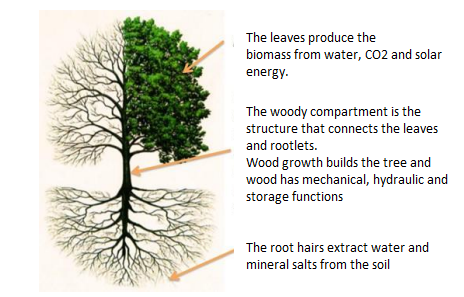
\includegraphics[width=8cm]{fig1}
	\caption{The main functions of the tree's wood, \cite{B.Thibaut}}
	\label{fig:fig1}
\end{figure}

The wood ensures in trees 3 main functions: the conduction of the raw sap from the roots to the branches, the mechanical support of the whole tree against its own weight and external forces, and the storage of nutrients such as starch. It is one of the few $100 \%$ natural materials. Its main chemical components are carbon, oxygen and hydrogen. Its use allows to limit greenhouse gas emissions and thus to fight against global warming. The tree absorbs carbon with which it manufactures the cells of the wood and rejects oxygen in the atmosphere. It is a natural material, renewable, transformable at low energy cost, recyclable, biologically degradable. For construction, it has advantages and disadvantages presented in table \ref{fig:fig2}:

\begin{comment}
\begin{table} \centering
	\begin{tabular}{cc}
		\toprule % horizontal line at the top of the table
		 The advantages and disadvantages of wood  \\\midrule
		The advantages & The disavantages \\\midrule
		Solidity and lightness: the strength-to-weight ratio is high. Its low density (500kg/m3) allows the use of less massive foundations.& Natural material and therefore has a high variability \\\midrule  
		Good thermal insulation: it is much less conductive than steel or concrete and reduces thermal bridges in buildings. & Orthotropic material \\\midrule
		Renewable and aesthetic. & Moisture-sensitive material \\\midrule
		Chemically inert. & Material sensitive to attack by insects and fungi \\\midrule
		Good fire behaviour: there is no toxic release, little heat transmission to neighbouring parts. Wood has a higher load-bearing capacity than steel. & Material that requires regular maintenance. \\ 
		\bottomrule % horizontal line at the bottom of the table
	\end{tabular}
	\caption{Orders of magnitude of axial compressive strengths and elastic moduli}
	\label{fig:fig13}
\end{table}
\end{comment}

\begin{table}[htp]
	\centering
	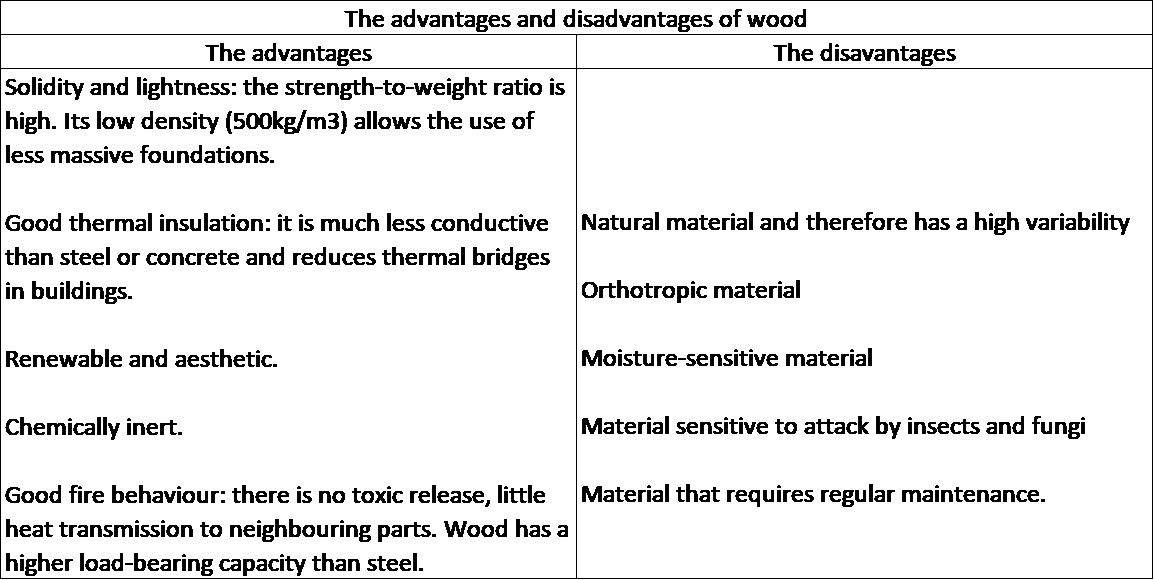
\includegraphics[width=12cm]{fig2}
	\caption{The advantages and disadvantages of wood}
	\label{fig:fig2}
\end{table}

\subsubsection{Two characteristics of the tree's wood}

Wood has two important characteristics which are anisotropy and heterogeneity. Anisotropy is a direct consequence of its heterogeneity.

\begin{itemize}
	\item It is heterogeneous in that it is composed of cells of different types and shapes. 
	\item It is anisotropic because its elements are oriented in several directions. Its mechanical and physical properties are not the same in all planes. The material is also orthotropic which means it has 3 preferred directions: longitudinal, radial and tangential.
\end{itemize}

In order to facilitate the studies on the physical and mechanical behaviours, we take as reference three types of sections as shown in figure \ref{fig:fig3} and defined as follows:

\begin{itemize}
	\item Cross-section (T), perpendicular to the shaft of the tree (trunk). When we look at a freshly felled tree, we can easily imagine a cross-section with the annual growth rings at the end, which correspond to the woody material produced by the tree in spring or summer.
	\item Tangential section (L), longitudinal, in the direction of the wood grain, and perpendicular to the medullary rays centered on the core of the log. During the cutting of the log into logs (current cutting), the patterns of the faces of the first boards obtained are characteristic.
	\item Radial section (R), again longitudinal, and in the direction of the wood grain, but parallel
	to the rays. This section can be seen on trays cut near the heart.
\end{itemize}


\begin{figure}[htp]
	\centering
	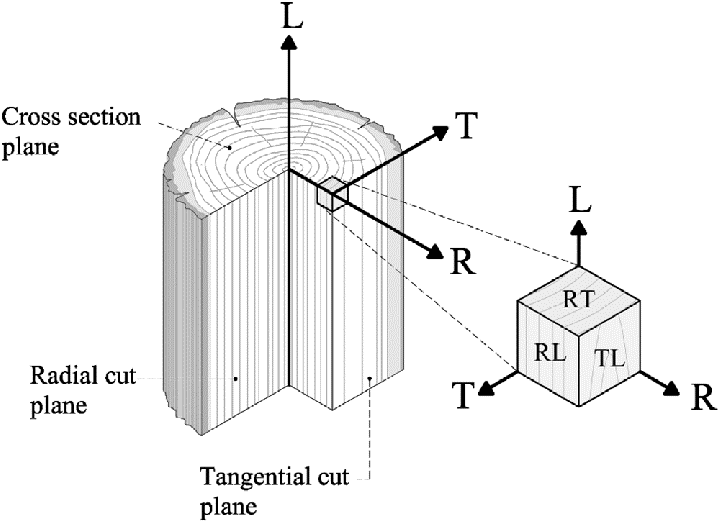
\includegraphics[width=10cm]{fig3}
	\caption{Main orthotropic directions and planes in Wood}
	\label{fig:fig3}
\end{figure}

\newpage

\subsection{Macroscopic and microscopic structure of wood}

\subsubsection{Macroscopic Scale}

The wood grows in concentric layers to the outside. It is this growth that creates heterogeneity \cite{Seddik2006phd}. Figure \ref{fig:fig4} shows the different elements that participate in the growth of a tree:


\begin{figure}[htp]
	\centering
	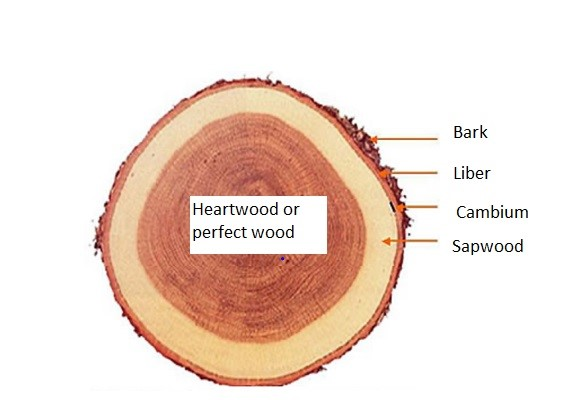
\includegraphics[width=10cm]{fig4}
	\caption{Sectional view of the wood}
	\label{fig:fig4}
\end{figure}

\begin{itemize}
	\item Outer bark: consists of dead cells and serves to protect the tree. It surrounds the tree to protect the cambium and the deep layer from climatic, animal or physical attack. 
	\item Inner bark (Liber): A layer of cells in which the elaborated (descending) sap circulates
	\item Cambium: Produces the bast towards the outside and the wood (xylem) towards the inside (growth tissue). This part can develop into sapwood or the next layer, the bark. It is therefore a particular part that explains the growth of the tree's circumference.
	\item Sapwood: Incompletely completed wood in which the raw sap circulates. The sap allows water and nutrients to be transmitted from the soil to all parts of the tree.
	\item Heartwood or perfect wood (dead cells) is the wood with the best mechanical properties. It is considered to be the dead part of the wood which is darker in colour than the other parts. It is the most used part of the tree for construction.
	\item Pith (heart) central part consisting of spongy tissue
\end{itemize}

There is sometimes a difference in colour between sapwood and heartwood (in the case of differentiated woods: oak, chestnut, pine, Douglas fir, larch). Sapwood is not or only slightly resistant to damage, whereas heartwood, which is not very impregnable, is naturally resistant. Conversely, for non-differentiated woods (fir, spruce, poplar, maple), the two parts are not visually distinguishable. However, there are different porosity and therefore different absorption capacities.

\subsubsection{Microscopic Scale}

Microscopically, there are two types of wood made up of different types of plant tissue: softwoods and hardwoods. Figure \ref{fig:fig5} presents microscopically these two categories of wood.

Softwoods are older than hardwoods and therefore have a simpler structure. They are made up of two main groups of cells: tracheids and parenchyma cells. The observation of these two types of cells shows the following configuration:

\begin{itemize}
	\item Tracheid fibers, having both support and conduction roles
	\item Rays: tracheid fibers and horizontal parenchyma
	\item Vertical parenchyma which ensure the distribution and storage of substances.
\end{itemize}

Hardwoods have more cell diversity than softwoods. They are composed of different cells: vessels, tracheids and parenchyma. The functions of support and conduction are performed by different cells:

\begin{itemize}
	\item Fibers (librifomes and tracheids): they are bundles of resistant cells, arranged in the axial direction, they ensure the rigidity and the mechanical resistance of wood. It is a bio composite made of cellulose, hemicellulose and ;
	\item Vessels: these are hollow cells that serve to conduct the raw sap from the roots to the leaves;
	\item Vertical parenchyma: this consists of parenchymal cells that contribute to the transport of nutrients. These parenchyma, associated with the vessels, give particular patterns to each species on the cross section;
	\item Woody rays (or medullary rays): these are horizontal parenchyma made up of thickened and lignified reserve cells with thickened and lignified walls. They accompany the vascular tissue. These cells participate in the support function of the tree. Their orientation is transverse and radiating from the longitudinal axis of the shaft.
\end{itemize}


\begin{figure}[htp]
	\centering
	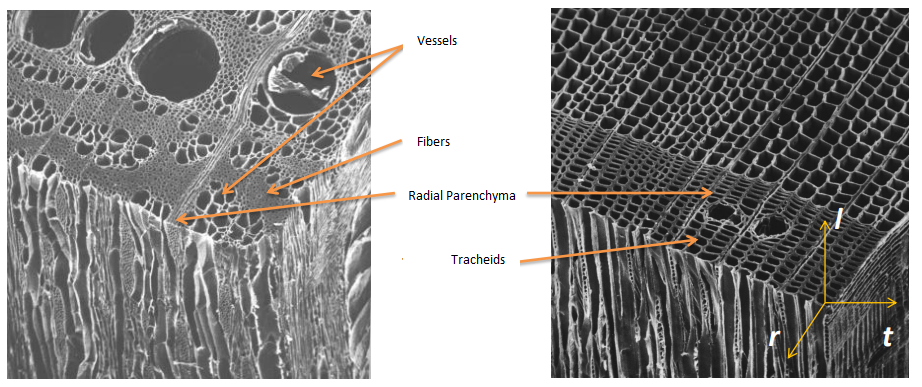
\includegraphics[width=12cm]{fig5}
	\caption{Microscopic section of hardwood and softwood, \cite{B.Thibaut}}
	\label{fig:fig5}
\end{figure}

\subsubsection{Chemical composition of wood}

Wood is a set of tissues of more or less hard consistency forming the main mass of the trunk of trees. It is an organized and heterogeneous material formed by a set of fibers accumulated by trees during their progressive growth over successive years. The structure of the tree is made up of cells (dead or alive) that ensure the circulation of sap, the storage of nutritive reserves and defense against possible aggressions.
The elemental chemical composition of wood organic matter varies very little from one species to another. On average, wood is made up of $50 \%$ carbon, $42 \%$ oxygen, $6 \%$ hydrogen, $1 \%$ nitrogen and $1 \%$ minerals. Wood is essentially composed of 3 types of polymers: cellulose, hemicelluloses and lignins. There are other components called extractives that do not contribute to the mechanical properties of the wood, but rather play the role of protection against the attacks of insects and other parasites.

\smallskip

\textbf{Lignin}

Its quantity in the wood represents $20 \%$ to $30 \%$. Lignin is a molecule that is part of the different components of wood. We found in some algae and in plants that have roots. It is the element which brings to wood its rigidity, its impermeability and its strength against decomposition. Trees are the plants that contain the most lignin. The lignin molecules allow the plants to stand upright to access to the light.

\smallskip

\textbf{Hemicelluloses}

The proportion of hemicelluloses in wood is estimated between $15 \%$ and $25 \%$. These are amorphous and branched polymers made up of units of different sugar residues. The hemicelluloses play a bridging role between the cellulose fibers.

\smallskip

\textbf{Cellulose}

It is the dominant constituent of wood (about $50 \%$). It is the most abundant organic matter on earth. The role of the fibrils, dispersed in an amorphous matrix of celluloses of a plastic nature, is to transform the latter into an elastic system with a high tensile strength, especially if the fibrils are small in diameter: about 2 nm in the primary walls.

\section{Mechanical behaviour}

In this section the physical and mechanical properties of wood are presented. Different factors influence the properties of wood such as the type of species, growing conditions and moisture content. Wood is considered to be an anisotropic material, meaning that its properties vary in different directions.The orthotropy, viscosity and moisture content of wood are three important characteristics and the mechanical characteristics of wood are directly related to these properties.

\subsection{The variability of wood}

One of the defects of wood is its natural origin. This gives it a great source of variability in its characteristics. In fact, there are two types of variability: that due to the species and that due to the growth of each individual within the same species. This means that criteria need to be established to classify wood and guarantee its structural characteristics. It is due to the growth mode of the trees (normal wood and reaction wood), to the variation of the seasons (spring wood and summer wood), to the annual climate (difference between the annual rings), to the different species (hardwoods and softwoods), to its anatomy, to its mechanical, hydric and thermal history...

The variability of the wood properties is also due to the growth mode of the tree which gives rise to two types of wood: normal wood and reaction wood. The difference between the two woods has been revealed by measuring growth stresses \cite{BrunoClair2003-2004}. Changes in stress states can be applied to the wood material depending on the mechanical stresses to which it is subjected (strong wind, unbalance of the trunk after the fall of a large branch, partial loosening of the trunk...). These changes in the state of stress in the wood are accompanied by a significant change in the structure of the wood cells during growth. The wood thus formed is called reaction wood, as opposed to normal wood.

\smallskip

\textbf{Compression wood}

Compression wood is produced almost exclusively by softwoods. It has a much darker color, which distinguishes it from normal wood to the naked eye. Physically, compression wood is much denser and can exceed the density of normal wood by 4/3. It should also be noted that compression wood has more shrinkage and swelling, and a lower fiber saturation point. From a mechanical point of view, compression wood is more resistant in bending and compression, but is also the most resilient.

\smallskip

\textbf{Tension wood}

Tension wood is found in hardwoods. Its density is generally higher than that of normal wood, up to $30 \%$ more. Note also that the longitudinal shrinkage is greater, which is one of the causes of the collapse phenomenon observed in tension wood. Finally, from a mechanical point of view, normal wood is more resistant to compression, bending, traction and shearing than the tension wood. This is due to the fact that the fibers of tension wood are thinner.

\subsection{The impact of humidity}

Wood has the particularity of having a moisture content that can vary and will lead to variable behaviour mechanically and with regard to its durability \cite{Taazount2021}.This rate has an influence: 

\begin{itemize}
	\item on the conservation of wood. If the rate is higher than $20 \%$, the wood is vulnerable to fungi and insects
	\item on the behaviour of parts and assemblies: variations in humidity lead to dimensional variations.
	\item On mechanical strength: the decrease in humidity makes the wood more resistant but also more fragile.
	\item On creep: moisture "softens" the wood.
\end{itemize}

The humidity is defined as the ratio of the mass of water it contains to its anhydrous mass \cite{Nguyen2016phd}. There are two ways to measure the moisture content of a piece of wood: either by weighing or by using a moisture meter. Below the two procedures are described:

By weighing: we determine by weighing the decrease in mass of a sample between current state and dry state then we calculate in percentage the ratio between this decrease in mass and the mass of the specimen.

Electrical measurement: moisture meters are designed on the same calculation basis. These devices calibrated in percentage of wood moisture give the value of wood moisture instantly. You just have to enter the density of the species and to put the device on the sample wood, then we read directly the value of the rate of moisture content.

The moisture content HI of each specimen can be expressed as a percentage by the formula \ref{eq:HI}:

\begin{equation}
	HI(\%) = \frac{M_{H}-M_{0}}{M_{0}}
	\label{eq:HI}
\end{equation}

where MH is the mass, in grams, of the specimen before drying. M0 is the mass, in grams, of the anhydrous specimen. Moisture exists in 3 forms in wood:

\smallskip

\textbf{The water of constitution}

It is an integral part of the wood material. It can only be released by the thermal degradation of the material. It is not taken into account in the measurement of moisture;

\smallskip

\textbf{The free water}

It is located in the cellular voids, in liquid form for very high humidities of wood, then in vapor form during and after drying;

\smallskip

\textbf{Bound water}

It permeates the cell walls. In these, the water molecules are "bound" to the cellulose and hemicellulose chains by electrical forces called "hydrogen bridges".

\smallskip

When all the free water is gone and all the bound water remains, the cell walls are still saturated with moisture and this is called the fiber saturation point (FSP). This saturation point varies between species and temperature. To have an idea at 20 degrees it is about 30\%. Below the FSP, humidity variations lead to dimensional variations. This variation is negligible in the longitudinal direction, but significant in the tangential direction. The consequences are important in the case of drying, which is accompanied by deformations both in the plane of the section and in the overall geometry of the part.


\begin{figure}[htp]
	\centering
	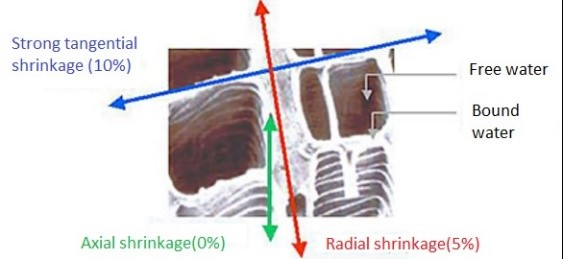
\includegraphics[width=10cm]{fig6}
	\caption{3 types of wood shrinkage}
	\label{fig:galaxy}
\end{figure}

\subsection{Influence of density on wood}

Density is the ratio of the density of wood to that of water. Wood can change in weight and volume as a result of moisture gain and loss. Generally the reference density is calculated with 12\% moisture. In fact, some researchers have shown that Young's modulus, Poisson's ratio and shear modulus depend on wood density. The density of wood varies from one species to another and also within the same species. The more fibers the wood has, the denser it is. If we take the example of balsa, it has a low proportion of fibers and therefore a low density. Conversely, panacoco has a high proportion of fibers and therefore has a high density \cite{Thibaut2015phd}.

\cite{BodigandJayne1982}  developed a formula \ref{eq:eq12} that relates the mechanical properties of the generalized Hooke's law to the density of wood by the relation :

\begin{equation}
	Y = a*D^b
	\label{eq:eq12}
\end{equation}

where Y represents the elastic properties, D is the density of the wood, a and b are two constants given in the charts for each wood species.

The density is expressed by the formula \ref{eq:eq13}:

\begin{equation}
	\rho = \frac{\rho_{woodspecimen}}{\rho_{4degreewater}}
	\label{eq:eq13}
\end{equation}

\subsection{Mechanical properties}

From a mechanical point of view, wood is an anisotropic material (= physical and mechanical properties depending on the direction considered) and orthotropic (it has 3 preferred directions: axial, radial, tangential). 

Wood is considered as an elastic material. It means that wood will return to its original shape or dimensions when the load causing the deformation is removed. Beyond this load limit, the wood does not regain its shape. It has then reached the plastic domain. It is the presence of cellulose that gives the wood a linear elastic behaviour. By drawing the stress-strain curve, it is possible to determine the Young's modulus E.


\begin{figure}[htp]
	\centering
	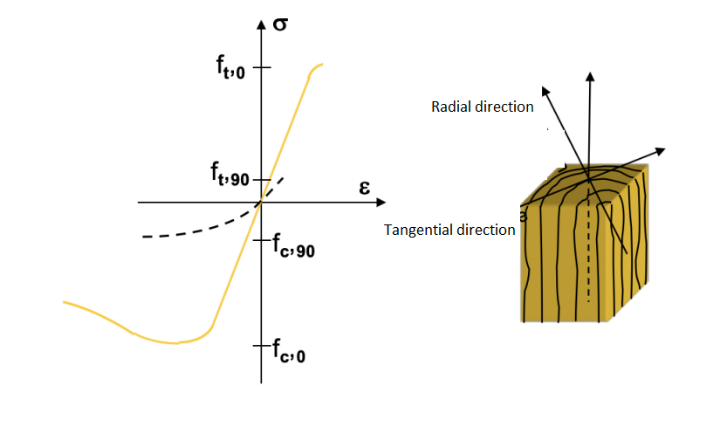
\includegraphics[width=10cm]{fig7}
	\caption{Orthotropy of wood without defects \cite{Taazount2021}}
	\label{fig:fig7}
\end{figure}

The curves in Figure \ref{fig:fig7} show the compressive and tensile behaviour of flawless wood loaded parallel to the fibres (solid line) and perpendicularly (dashed line) at a constant strain rate. Cellulose provides high mechanical properties in the longitudinal direction, as this is the direction in which it is oriented. In the transverse direction, the little cohesion provided by the lignin is not sufficient to hold the fibres together, only the radial tracheids provide a little strength. It can be said that wood without defects has a strong anisotropy. It is rigid and strong parallel to the fibres, sensitive to splitting and has low shear strength \cite{Taazount2021}.

Considering a one-dimensional behavior model in the direction of the fibers, we can write \ref{eq:eq14} :

\begin{equation}
	\sigma = E_{L}*\epsilon
	\label{eq:eq14}
\end{equation}

With the proportionality between the stress $\sigma$ and the deformation $\epsilon$ along the fiber axis with respect to the wood grain, $ E_L $ represents the "longitudinal modulus of elasticity" which must in all rigor be characterized for each load case in tension, compression, bending etc.


\textbf{Compressive behaviour}

In order to determine the behaviour of the material in compression, it must be stressed in both directions (parallel and orthogonal to the fibres). This is known as axial compression and transverse compression. The test is carried out on a parallelepipedic specimen, 20 x 20 x 60  with a loading speed of 40 MPa/mm. The variation of the stress as a function of the strain is plotted on the figure \ref{fig:fig8}.


\begin{figure}[htp]
	\centering
	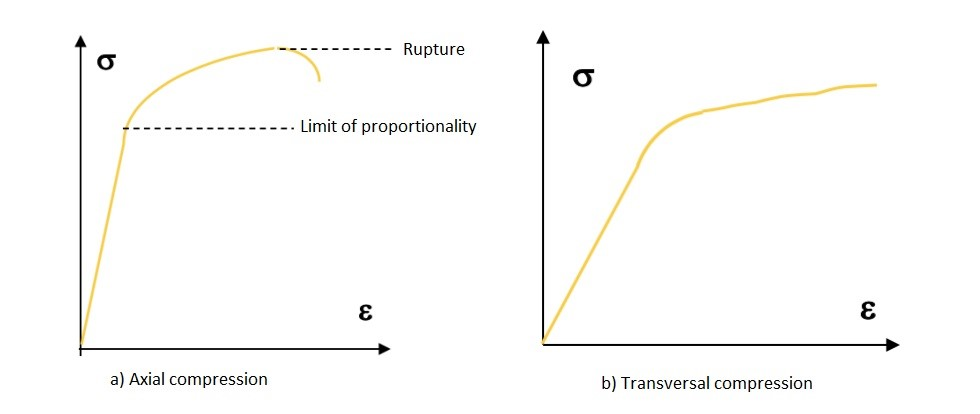
\includegraphics[width=10cm]{fig8}
	\caption{Axial and transverse compression of wood}
	\label{fig:fig8}
\end{figure}

Orders of magnitude of axial compressive strengths and elastic moduli can be given for each type of wood species in table \ref{fig:fig9}. 

\begin{table} \centering
	\begin{tabular}{ccc}
		\toprule % horizontal line at the top of the table
		& Resinous wood & Deciduous wood  \\\midrule
		Axial compression strength & 45 \unit{\mega\pascal}
		& 55 \unit{\mega\pascal} \\\midrule
		Elasticity modulus & 12000 \unit{\mega\pascal}
		& 14000 \unit{\mega\pascal} \\
		\bottomrule % horizontal line at the bottom of the table
	\end{tabular}
	\caption{Orders of magnitude of axial compressive strengths and elastic moduli}
	\label{fig:fig9}
\end{table}


For transverse compression and regardless of the wood species, the strength is divided by 7 (i.e. strength < 10 MPa). 

The strength of the wood can then be assessed if it is loaded obliquely, i.e. the direction of loading is at an angle of 0 to 90° to the direction of the fibres. 


\begin{figure}[htp]
	\centering
	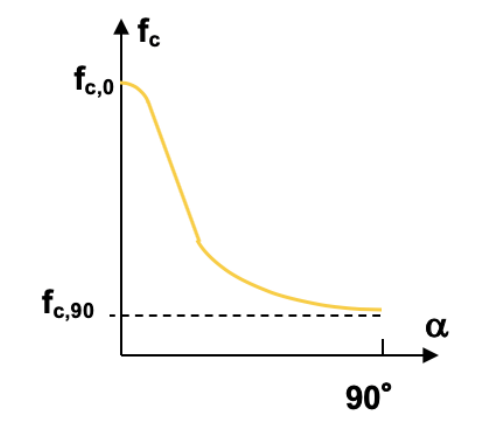
\includegraphics[width=8cm]{fig10}
	\caption{Variation of the compressive strength of wood as a function of the load angle}
	\label{fig:fig10}
\end{figure}

Figure \ref{fig:fig10} shows the variation of the compressive strength of wood as a function of the load angle. It can be seen that the strength is maximum for a load parallel to the fibres (fc,0) and minimum for a load perpendicular to the fibres (fc,90). Theoretically, the compressive strength can be evaluated as a function of this angle using the Hankinson formula. A similar formula \ref{eq:eq15} exists for the modulus.

\begin{equation}
	\sigma_{\alpha} = \frac{\sigma_{0}*\sigma_{90}}{\sigma_{\alpha}*sin(\alpha)^2+\sigma_{90}*cos(\alpha)^2}
	\label{eq:eq15}
\end{equation}

\textbf{Tensile behaviour}

Wood has an almost elastic tensile behaviour until it breaks. Its tensile elastic modulus is equivalent to that in axial compression. The breaking stress is up to twice as high as that in compression. We can retain $f_{t0}=80$ to 140 MPa.


\begin{figure}[htp]
	\centering
	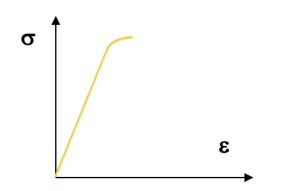
\includegraphics[width=8cm]{fig11}
	\caption{Variation of the axial tensile stress of wood with deformation}
	\label{fig:galaxy}
\end{figure}

In the same way as for compression, the oblique tensile strength can be theoretically evaluated using the Hankinson formula. However, these values are strongly influenced by the presence of knots and the possible slope of the wood grain.

\smallskip

\textbf{Shearing behaviour}

In order to measure the shear strength of wood in the longitudinal direction, a preferential shear plane must be created by the shape of the specimen. This is illustrated in Figure \ref{fig:fig12} :


\begin{figure}[htp]
	\centering
	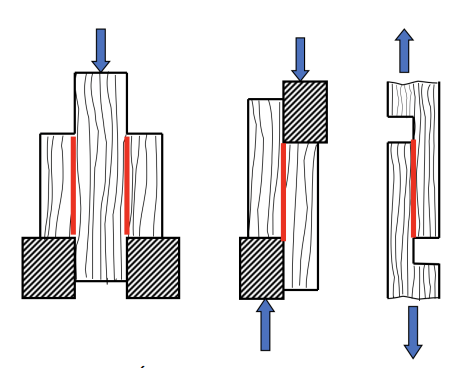
\includegraphics[width=8cm]{fig12}
	\caption{Wood shearing}
	\label{fig:fig12}
\end{figure}

In the figure, the light areas represent the wood, the dark areas represent the blocking points (prevented displacement) and the arrows represent the stresses. These experimental set-ups allow the creation of shear planes (in red). These shear strength values can be retained in table \ref{fig:fig13} :

\begin{table} \centering
\begin{tabular}{cccc}
	\toprule % horizontal line at the top of the table
	& Resinous wood & Soft deciduous wood & Hard deciduous wood \\\midrule
Shear strenght & 2.5 -- 3.5 \unit{\mega\pascal}
	& 3 -- 5 \unit{\mega\pascal} & 5 -- 7.5 \unit{\mega\pascal}\\
	  \bottomrule % horizontal line at the bottom of the table
\end{tabular}
	\caption{Shear strenght values}
	\label{fig:fig13}
\end{table}

%
%\begin{table}[htp]
%	\centering
%	
\includegraphics[width=10cm]{fig13}
%	\caption{Shear strenght values}
%	\{fig:fig13}
%\end{table}


\section{Fracture mechanic of wood}

\subsection{Test pieces used in fracture mechanics}

There are three ways of applying a force to allow a crack to propagate as shown figure \ref{fig:fig14}. Mode I is a tensile stress normal to the crack plane, mode II is a shear stress acting parallel to the crack plane and perpendicular to the crack front. Mode III is a shear stress acting parallel to the crack plane and parallel to the crack front. In general, a crack propagates in a material under a combination of stresses in all three modes. These modes can be presenting by the energy release rate (G) linked to crack length. It is called R-curve and has three characterized propagation crack zones. A first increasing phase of instability to initiate the cracking process. A second phase, which corresponds to a stabilised propagation range during which only viscoelastic effects (creep) will participate in the advance of the crack front and a last phase which symbolises the ruin of the material.


\begin{figure}[htp]
	\centering
	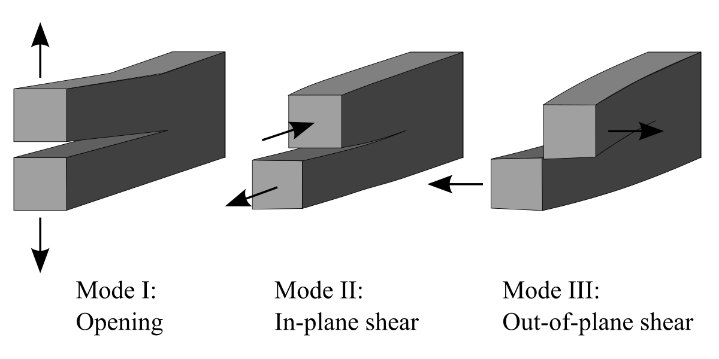
\includegraphics[width=10cm]{fig14}
	\caption{Illustration of the three modes of rupture}
	\label{fig:fig14}
\end{figure}

Moreover, the cracking failure mechanism can occur in two types of cracking: 

\begin{itemize}
	\item Abrupt cracking: for solids, or for very high strength materials, the working stresses are very high, and considerable potential energy is thus created; the presence of small cracks can then lead to abrupt failure which is often not accompanied by macroscopic plastic deformations due to the very low ductility. 
	\item Successive cracking: this is a succession of mechanisms (brittle - ductile) which, under repeated stresses, leads to successive cracking or fatigue failure. The factors that influence the cracking behaviour of materials are of two kinds: metallurgical and mechanical. The mechanical factors relate to the state of displacements, strains and stresses, as well as environmental conditions such as temperature or relative humidity. It is easier to observe because it takes more time to involve samples destruction than a unique and sudden crack. With a material like wood, successive cracks rupture are expected.
\end{itemize}

In order to realize these different modes of rupture, we need specimens that meet certain criteria such as geometry. Indeed, some specimens were designed to solve problems for mode I while others for mode II or mixed mode. There are therefore several types of test specimens:

\textbf{DCB test piece}

The double cantilever beam (DCB) specimen was developed for testing in the crack opening mode (Mode I). Its design allows to obtain a stress intensity factor that decreases when the crack propagates. However, it also allows the determination of the toughness and the critical energy restitution rate in mode I and mode II. Indeed, in the document of \cite{YoshiharaandNobusue2008} Mode I and Mode II fracture toughness were measured of compressed spruce by a double cantilever beam (DCB) test and a three-point bend end notched flexure (3ENF) test figure \ref{fig:fig15}.


\begin{figure}[htp]
	\centering
	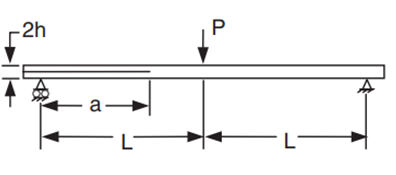
\includegraphics[width=.6\textwidth]{fig15}
	\caption{Schematic representation of 3ENF test with DCB test piece. \cite{DavidsonandSun2005}}
	\label{fig:fig15}
\end{figure}

\newpage
\textbf{Double Cantilever Beam specimen with variable inertia}

The classical DCB specimen had an instability from the beginning of the crack initiation. This is why \cite{Dubois2002} proposed a variable inertia DCB specimen with crack stability. The DCB specimen with variable inertia figure \ref{fig:fig16} was designed to ensure stabilised propagation in Mode I. Thus, after the crack initiation zone, a decrease in the rate of elastic energy restitution G is observed over a given propagation range. During this phase, only viscoelastic effects will participate in the progression of the crack front when the specimen is loaded in creep. The viscoelastic characteristics will thus be clearly decoupled from the cracking parameters. 


\begin{figure}[htp]
	\centering
	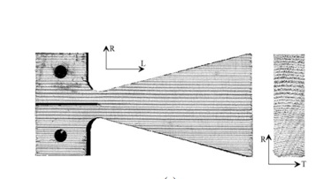
\includegraphics[width=.6\textwidth]{fig16}
	\caption{DCB specimen with variable inertia \cite{Dubois2002}}
	\label{fig:fig16}
\end{figure}


\textbf{Compact Tension Shear specimen}

The Compact Tension Shear (CTS) specimen figure \ref{fig:fig17} is designed to evaluate all mixed modes in different materials. It was developed for mixed loads in isotropic materials. Two steel arms are pierced with holes where symmetrical forces P oriented by angles $\beta$ of mixtures are applied. On both specimens, the crack remains oriented in the direction of high orthotropy.

\begin{figure}[tp]
	\centering
	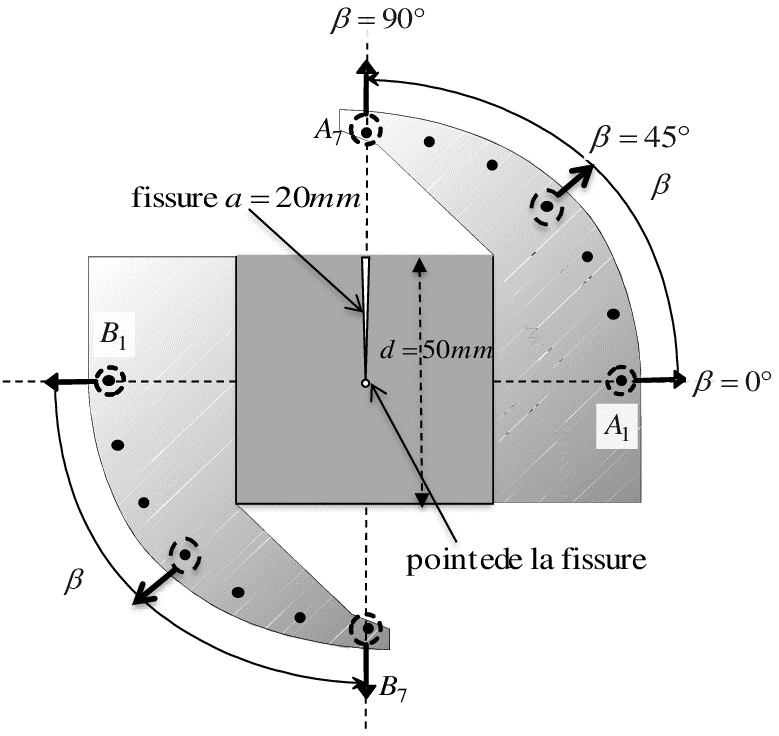
\includegraphics[width=.4\textwidth]{fig17}
	\caption{Compact Tension Shear (CTS) specimen}
	\label{fig:fig17}
\end{figure}

\textbf{Mixed Mode Crack Growth specimen}

The design of the Mixed Mode Crack Growth (MMCG) specimen figure \ref{fig:fig18} was based on a combination of the two geometric solutions described above. The original DCB specimen was modified by adding a lower heel to secure the mixed mode loading device. The upper heel was slightly inclined to ensure stiffness in the vicinity of the two connection fillets. The body of the specimen has increasing inertia towards the crack tip to ensure a stable rate of energy restitution. Four symmetrically arranged PVC arms are attached to the wooden specimen. Boreholes are provided to allow for loads with a variable $\beta$-mixing rate identical to that of the CTS specimen. This test piece allows for a given propagation range, in mode 1, mode 2 and in mixed mode, a stability or even a considerable decrease of the energy restitution rate\cite{MoutouPitti2008}.





\begin{figure}[tp]
	\centering
	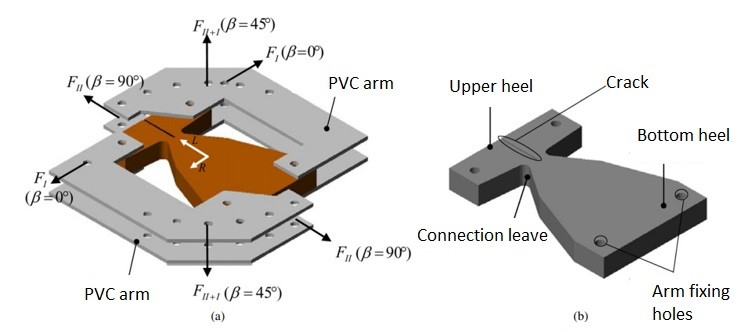
\includegraphics[width=.6\textwidth]{fig18}
	\caption{2MCG test piece \cite{MoutouPitti2008}}
	\label{fig:fig18}
\end{figure}

\subsection{Stress and strain fields}

It is important to notice that different zones are studied. In fracture mechanics, three successive zones visible figure \ref{fig:fig19} can be distinguished schematically in a cracked medium:

\begin{itemize}
	\item The development zone or zone 1: the zone closest to the crack tip. In this part the material is very damaged, which makes its mechanical evaluation rather complex. The size of this zone determines the type of cracking that will occur. Indeed, if the size of the zone is large, ductile cracking will be observed. On the other hand, if it is small, brittle cracking will be observed.
	\item The singular zone or zone 2: this covers the entire development zone. In this zone, the displacement, strain and stress fields are continuous and have a formulation that is independent of the distant geometry of the structure. The material has a linear viscoelastic behaviour. Its boundary with zone 1 is assumed to be continuous in stress and displacement.
	\item The far zone or zone 3: this is the zone furthest from the crack. It connects the singular zone with the loading and displacement boundary conditions.
\end{itemize}


\begin{figure}[htp]
	\centering
	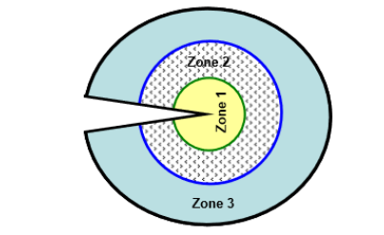
\includegraphics[width=10cm]{fig19}
	\caption{Cracking zone \cite{MoutouPitti2008phd}}
	\label{fig:fig19}
\end{figure}

For a linear elastic material, the stress field at a point M in the vicinity of the crack can be expressed simply as a function of the stress intensity factor $K_{I,II,III}$ and the polar coordinates ( r, $\theta$). The dimensionless functions $f_{ij}$  and  $g_{ij}$ depend on the mode of loading. The intensity factor is independent of the point M. Moreover, in the vicinity of the crack tip the value of r is very small, and tends to 0. Thus the stress field is expressed by \ref{eq:eq16}:

\begin{equation}
	\sigma_{i,j} = \frac{K_{\beta}}{\sqrt{2*\pi*r}}*f_{i,j}(\theta)
	\label{eq:eq16}
\end{equation}

The coefficient $K_\beta$ in the equation \ref{eq:eq16} is the stress intensity factor (mode I and mode II) and is independent of the point M, Figure \ref{fig:fig20}.


\begin{figure}[htp]
	\centering
	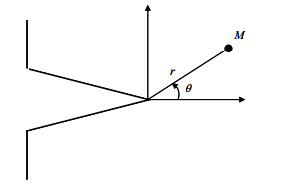
\includegraphics[width=8cm]{fig20}
	\caption{Crack tip scoring}
	\label{fig:fig20}
\end{figure}

We have seen that there are three ways of applying a force, to a specimen, to allow a crack to propagate. These modes define the expression of the mechanical field in zone 2 for orthotropic material \cite{Odounga2018phd}. They are defined and expressed as follows and are illustrated in Figure \ref{fig:fig14}:

\textbf{Mechanical fields in the singular zone for mode 1}

\begin{equation}
	\sigma_{1,1} = \frac{K_{1}}{\sqrt{2 \pi r}} \cos{\frac{\theta}{2}}  \left( 1-\sin{\frac{\theta}{2}} \sin{\frac{3 \theta}{2}} \right)
	\label{eq:eq17}
\end{equation}

\begin{equation}
	\sigma_{2,2} = \frac{K_{1}}{\sqrt{2 \pi*r}} \cos{\frac{\theta}{2}}  \left( 1+\sin{\frac{\theta}{2}} \sin{\frac{3 \theta}{2}} \right)
	\label{eq:eq18}
\end{equation}

\begin{equation}
	\sigma_{1,2} = \frac{K_{1}}{\sqrt{2 \pi r}} \cos{\frac{\theta}{2}}  \sin{\frac{\theta}{2}} \cos{\frac{3 \theta}{2}}
	\label{eq:eq19}
\end{equation}

The displacement field for the mode 1 loading is written as follows:

\begin{equation}
	u_{1} = \frac{K_{1}}{4 \pi}*\sqrt{\frac{r}{2 \pi}} \left((2 \chi-1) \sin{\frac{\theta}{2}}-\sin{\frac{3 \theta}{2}}\right)
	\label{eq:eq110}
\end{equation}

\begin{equation}
	u_{2} = \frac{K_{1}}{4 \pi} \sqrt{\frac{r}{2*\pi}} \left((2 \chi+1) \sin{\frac{\theta}{2}}-\sin{\frac{3 \theta}{2}}\right)
	\label{eq:eq111}
\end{equation}

With : 

$K_1$  the mode 1 stress intensity factor

$\mu=\frac{E}{2 (1+\nu)}$ , the shear coefficient of Lame

$\nu=\frac{\lambda}{2 (\lambda+\mu)}$ , the shear coefficient of Poisson

$E=\frac{\mu (3 \lambda+2 \mu)}{\lambda+\mu}$, the Young modulus

$\lambda=\frac{\nu E}{(1-2 \nu)(1+\nu)}$ , the Lame’s Coefficients

The term $\chi$ is a constant defined as follows:\ $\chi=3-4\nu$ for plane deformations and \ $\chi=\frac{3-\nu}{1-\nu}$  for plane stresses.

r and $\theta$ polar coordinates of point M centred on the crack tip, Figure 11

\smallskip

\textbf{Mechanical fields in the singular zone for mode 2}

\begin{equation}
	\sigma_{1,1} = \frac{-K_{2}}{\sqrt{2 \pi r}} \sin{\frac{\theta}{2}}  \left( 2+\cos{\frac{\theta}{2}} \cos{\frac{3 \theta}{2}} \right)
	\label{eq:eq112}
\end{equation}

\begin{equation}
	\sigma_{2,2} = \frac{K_{2}}{\sqrt{2 \pi r}} \cos{\frac{\theta}{2}}  \sin{\frac{\theta}{2}} \cos{\frac{3 \theta}{2}}
	\label{eq:eq113}
\end{equation}

\begin{equation}
	\sigma_{1,2} = \frac{K_{2}}{\sqrt{2 \pi r}} \cos{\frac{\theta}{2}}  \left( 1-\sin{\frac{\theta}{2}} \sin{\frac{3 \theta}{2}} \right)
	\label{eq:eq14}
\end{equation}

The displacement field for the mode 2 loading is written as follows:

\begin{equation}
	u_{1} = \frac{-K_{2}}{4 \pi} \sqrt{\frac{r}{2 \pi}} \left((2 \chi+3) \sin{\frac{\theta}{2}}+\sin{\frac{3 \theta}{2}}\right)
	\label{eq:eq115}
\end{equation}

\begin{equation}
	u_{2} = \frac{K_{2}}{4 \pi} \sqrt{\frac{r}{2 \pi}} \left((2 \chi+3) \cos{\frac{\theta}{2}}+\cos{\frac{3 \theta}{2}}\right)
	\label{eq:eq117}
\end{equation}

With : $K_2$  the mode 2 stress intensity factor

\smallskip

\textbf{Mechanical fields in the singular zone for mode 3}

\begin{equation}
	\sigma_{1,3} = \frac{-K_{3}}{\sqrt{2 \pi r}} \sin{\frac{\theta}{2}}
	\label{eq:eq118}
\end{equation}

\begin{equation}
	\sigma_{2,3} = \frac{K_{3}}{\sqrt{2 \pi r}} \cos{\frac{\theta}{2}}
	\label{eq:eq119}
\end{equation}

The displacement field for the mode 3 loading is written as follows:

\begin{equation}
	u_{3} = \frac{-2 K_{3}}{\mu} \sqrt{\frac{r}{2 \pi}} \sin{\frac{\theta}{2}}
	\label{eq:eq120}
\end{equation}

With : $K_3$  the mode 3 stress intensity factor

\subsection{Method of the complacency}

In this part we give and define the different terms of the imposed displacement complacency formula. This formula will be used in the next chapters to calculate the energy restitution rate. It is defined by the ratio of two parameters: the variation of energy per unit area cracked and the crack propagation in a linear elastic material. The crack propagation will occur when the energy G reaches a critical value noted Gc. This value Gc is a measure of the toughness of the material. Let us now define the mathematical expression of G. First, let us consider a material with a crack of length a and thickness b. A crack propagation $\Delta$a will be accompanied by the following energy variations \ref{eq:eq121}:

\begin{equation}
	\Delta W_{ext}=\Delta W_{elast}+\Delta U
	\label{eq:eq121}
\end{equation}

With:

$\Delta W_{ext}$ the applied energy change (due to external forces)

$\Delta W_{elast}$ the change in dissipated energy 

$\Delta$U the energy expended during crack propagation over the length $\Delta$a.

The energy G reported to the unit area will be \ref{eq:eq122} :

\begin{equation}
	G = \lim_{\Delta \to 0}= \frac{\Delta U}{\Delta A}= \frac{\partial U}{\partial A}
	\label{eq:eq122}
\end{equation}

Where $\Delta A=b\Delta a$  is the cracked area during crack propagation. b is usually equal to 1 because a unit thickness is often considered. Therefore, the energy per unit thickness will be of the form \ref{eq:eq123} :

\begin{equation}
	G = \lim_{\Delta \to 0}= \frac{\Delta U}{\Delta a}= \frac{\partial U}{\partial a}
	\label{eq:eq123}
\end{equation}

In order to understand the meaning of the energy restitution rate, we will consider, from an initial configuration, the propagation (in a specimen of unit thickness) in the following two classical cases (Figure 18):

\begin{itemize}
	\item propagation with imposed displacement d ; 
	\item propagation with imposed force F.
\end{itemize}

\begin{figure}[htp]
	\centering
	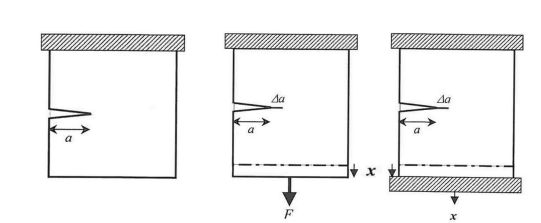
\includegraphics[width=10cm]{fig21}
	\caption{Stable propagation with imposed force or imposed displacement \cite{Zeghloul2001phd}.}
	\label{fig:fig21}
\end{figure}

In our work we will limit ourselves to the case of propagation with imposed displacement. In this case if $\Delta x=0$ (with $\Delta x$ variation of the crack), the external energy variation will be zero, we then deduce the elastic energy :

$W_{elast}=\frac{Fx}{2}$

By introducing the complacency by the relation :

$C=\frac{x}{F}$

We deduce :

$W_{elast}=\frac{CF^2}{2}=\frac{x^2}{2C}$

$\Delta W_{elast}=\frac{\partial W_{elast}}{\partial a}\Delta a=\frac{\partial W_{elast}}{\partial a}\ \frac{\partial C}{\partial a}\Delta a=\frac{-x^2}{2C^2}\ \frac{\partial C}{\partial a}\Delta a$

And because we have:

$\Delta W_{ext}=0=\Delta W_{elast}+\Delta U\leftrightarrow \Delta U =-\Delta W_{elast}$

Then we have:

$\Delta U=\frac{x^2}{2C^2}\ \frac{\partial C}{\partial a}\Delta a$

Which enables to obtain \ref{eq:eq124}:

\begin{equation}
	G=\frac{x^2}{2C^2}\ \frac{\partial C}{\partial a}=\frac{F^2}{2}\ \frac{\partial C}{\partial a}
	\label{eq:eq124}
\end{equation}

The relationship in equation \ref{eq:eq124} is related to the unit thickness. In the case where $b\neq1$
we obtain \ref{eq:eq125}:

\begin{equation}
	G_c=\frac{{F_{ci}}^2}{2b}\ \frac{\partial C}{\partial a}
	\label{eq:eq125}
\end{equation}

With:

$G_c$ the value of energy release rate (in $J/mm^2$)

$F_{ci}$ the critical force which involves the crack (in N)

b the thickness of the specimen (in mm)

C the complacency evolution (in ${Pa}^{-1}$)

a the crack length evolution (in mm)



\section{Software and DIC method}

\subsection{Dic method}

Digital image correlation (DIC) was developed in 1983. It is a 2D or 3D optical method that measures displacements between two images. It is increasingly used in materials science to determine strain fields, detect cracks or to provide displacement fields for material property identification procedures. It is a non-contact optical method of measuring kinematic fields, based on the comparison of the signal amplitude. It relies on the grey levels of the images. The particles are optically tracked using computer algorithms to determine displacements and velocities. Rather than tracking moving particles in a fluid, DIC tracks changes in the relative position of the high contrast surface finish. It works by comparing two images, one reference and one deformed, taken during loading. Thus it must detect a pattern in the reference image and compare it to the pattern in the other images \cite{Mambili2018}. The DIC formulation relies on the conservation of grey levels between the two instants at which the reference images S0 and the current images St are recorded. In other words, this principle is based on the comparison between a reference image and a distorted image. Each image is composed of pixels, and each pixel as a function of the light flux returns information. For 8-bit images, for example, a pixel can have a value between 0 for black and 255 for white. Each image is therefore stored in the form of a two-dimensional matrix whose cells correspond to a value. These matrices are the image correlation data. DIC compares these matrices and deduces the surface displacement field. To do this, during the analysis, the algorithm in place searches for a correlation zone, predefined in the reference image, in that of the image in the deformed state figure \ref{fig:fig22}.


\begin{figure}[htp]
	\centering
	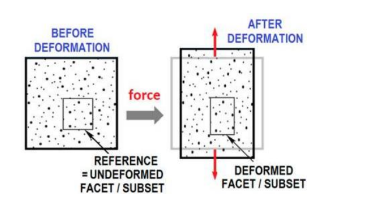
\includegraphics[width=10cm]{fig22}
	\caption{Example of captured images obtained by a camera for image analysis.}
	\label{fig:fig22}
\end{figure}

The system consists of a digital camera and specialised computer software like MatchID. The camera is used to capture consecutive images of the surface of the sample under test before and during the deformation test. The digital images thus determined, which correspond to a series of photographs, are analysed by the DIC software. Displacement maps of the sample on the surface are created. The stress fields can be evaluated from the strain fields. The formula used to obtain the displacement field is shown below equation \ref{eq:eq126}:

\begin{equation}
	u^k=\left[{u_z^k\atop u_y^k}\right]=\sum_{i=1}^{N}\left\{\left[{{\ \ f}_i\left(k,\Phi_k\right)\ \ {\ \ g}_i\left(k,\Phi_k\right)\atop{\ \ l}_i\left(k,\Phi_k\right)\ \ {\ \ m}_i\left(k,\Phi_k\right)}\right]\times\left[{A_1^i\atop A_2^i}\right] \times r_k^{i/2}\right\}+\left[{T_x\atop T_y}\right]+R\times\left[{y_k\atop x_k}\right] 
	\label{eq:eq126}
\end{equation}

With the polar functions $f_i$, $g_i$, $l_i$, $m_i$, k depends on the material because of the Poisson's ratio term which determines k. The T terms are correction factors for rigid body movements.

It is important to note that the 2D orthotropic elastic material model used for wood requires five engineering constants as input parameters in image analysis systems. These inputs are specific to the software used and include the Young's modulus in the longitudinal direction ($E_L=E_1$), the transverse Young's modulus ($E_{trans}=E_R=E_T=E_2$), and the shear modulus ($G_{LR}=G_{LT}=G_{12}$) if the shear mode is being studied.
The Poisson's ratio $\nu$ is also a necessary input and may vary depending on whether the surface being studied is in or out of the plane. Additionally, the initial crack length must be input into the model.
Three main inputs are required to describe damage, although this may vary depending on the software being used. For mode I damage, the damage initiation stress ($\sigma_{ini}$), the failure stress ($\delta_{fl}$), and the shape coefficient of the exponential function ($\alpha_l$) are used to describe the damage.

\subsection{Uncertainty Quantification}

There are two types of errors in DIC measurements, namely variance errors and bias errors. The main sources of noise in DIC measurements are camera noise and matching errors during the correlation process. Bias can be introduced by smoothing of spatial gradients in a QOI, uncorrected lens distortions, poor camera calibration, and out-of-plane motion in 2D-DIC measurements, to name a few sources. Establishing the uncertainty of the QOIs accounting for bias and noise errors is essential for intelligent evaluation and use of DIC results. Without quantifying the uncertainty, it is impossible to know whether a reported QOI value is meaningful and relevant, or whether it is the result of random noise and bias.

Bias errors are often difficult to quantify, as the true value of a QOI is usually not known. However, some sources of bias can be assessed. Even if no bias errors are detected, unknown bias errors may still exist.

The process of quantifying variance errors is often called noise floor analysis. The basic idea of a noise floor analysis is to correlate static images of a DIC pattern that were acquired under the same conditions as the test images. With no force applied or displacement on the test piece, all measured QOIs requiring deformation are errors. The same user-selected DIC parameters that are used for the analysis of the test piece images during deformation should also be used for the analysis of the noise floor images. Therefore, the final noise floor analysis is typically performed after the mechanical test image analysis, but using the images acquired immediately before the mechanical test.
Two different metrics can be used to quantify the variance error of the QOIs: a spatial standard deviation and a temporal standard deviation. It is recommended that both spatial and temporal standard deviations are calculated and evaluated to see if one is significantly larger than the other. However, the spatial and temporal standard deviations are generally similar, and a single metric or the average of the two metrics can be selected to quantify the noise floor. 

%To quantify the spatial variation of the QOI, compute the standard deviation of the QOI for each image and average this spatial standard deviation over time for all static images. To quantify temporal variation, calculate the standard deviation of the QOI for each subset over time and average this temporal standard deviation for each subset over all subsets in the image ZOI.

\section{Conclusion}

This chapter have provided a better understanding of the material wood. Its definition, its various functions, its physical and mechanical properties were reminded as well as the elements which constitute it at the macroscopic and microscopic level. Moreover, it was also recalled the various parameters such as moisture that can influence the physical and mechanical characteristics of wood.
This chapter recalled also some basics of fracture mechanics and different specimens used for the observation of crack propagation. In particular, it explains the choice of using the 2MCG specimen for the tests. It also recalls the basic formulas of linear fracture mechanics in orthotropic field such as the stress intensity factors and the energy restitution rate. In addition, the field measurement method called DIC was presented and the procedure to obtain the crack propagation was explained. The next chapter will present the applied experimental method.



\chapter{Pre and post processing work preparation}
\label{Chapter2}

\section{Introduction}

This chapter focuses on the proposed methodology for analysing the mechanical fracture tests. It comprehensively explains the equipment for conducting the tests and the necessary preparations. A dedicated section is devoted to elucidating the application of the DIC method and the appropriate utilisation of MatchID software. Moreover, it outlines crucial DIC setting parameters, including subset size, step size, correlation criteria, and shape functions, to ensure optimal accuracy in the DIC analysis while balancing out the spatial resolution and precision.
Furthermore, this chapter introduces two fracture analysis methods, each accompanied by a custom-developed Python code. A comparative assessment of these methods is presented, allowing for a judgment regarding their relative effectiveness and merits.

\section{Material and testing}

\subsection{MMCG fracture test}

The MMCG specimen was initially developed by \citet{MoutouPitti2008}. However, it should be noted that the specimens tested in this work have different dimensions compared to the original design. Upon meticulous measurements, it was discovered that the tested specimens in this study share the exact dimensions as those examined by \citep{Odounga2018phd}. The dimensions of the specimens to be tested are provided in Figure \ref{fig:fig23}.

\begin{figure}[htp]
	\centering
	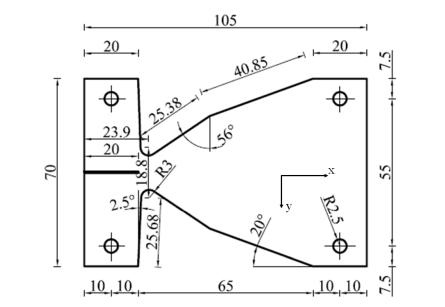
\includegraphics[width=.6\textwidth]{fig23}
	\caption{Dimensions of the tested MMCG specimen \citep{MoutouPitti2008, Odounga2018phd}.}
	\label{fig:fig23}
\end{figure}

\subsection{Wood characteristics}

For the tests conducted in this thesis, the chosen European species is the silver fir, which belongs to the category of coniferous trees. This softwood species is predominantly found in the northern hemisphere, similar to pines and other aged trees. Its name originates from the white colour of its wood, and its circumference typically ranges from 50 to 80 cm. According to CIRAD data, the silver fir exhibits a density of 0.45 to 0.60, a saturation fiber point (SFP) of approximately 30\%, and a compressive strength of 41 MPa. Notably, it experiences significant tangential shrinkage at 8.7\%, while the radial shrinkage measures 4\%. Silver fir wood is commonly utilised for framing, columns, and light structures due to its strength, although it requires treatment to prevent fungal and insect attacks. However, water pockets within the tree and its susceptibility to splitting pose concerns that may limit the use of specific connectors in construction.
Wooden specimens were carefully characterised before testing by measuring weight, density, and moisture content. Before the tests, the samples were weighed, denoted as $M_H$, to determine their mass during testing. The wood density can also be derived from the sample's volume and mass. AutoCAD was employed to create a digital representation of the sample, enabling us to determine its theoretical surface, which can then be multiplied by the thickness to calculate the volume. The density of each sample can be determined by applying the formula $\rho = M/V$.
After testing, the specimens were placed in an oven set at 100 degrees until their mass, labelled as $M_C$, stabilised. Two specimens were subjected to this process for 73 hours, and various measurements were taken until a constant mass was achieved. The moisture content of the specimens can be determined using equation \ref{eq:HI}. Consequently, we possess the mass, density, and moisture content values necessary to compare our results with the literature review, as presented in Table \ref{tab:Tabmean}.

\begin{table}[h]
	\centering
	\begin{tabular}{lcl}\toprule
		Mass of the specimens, MH [g] && 29.83  \\
		Volume, V [cm$^3$] && 6916  \\
		Density, $\rho$ [kg/m$^3$] && 431.3  \\
		Moisture Content, HI [\%] && 10.3 \\\bottomrule
	\end{tabular}
	\caption{Characteristics of MMCG Silver Fir specimens.}
	\label{tab:Tabmean}
\end{table}

\subsection{Arcan solid model and grips}

An  Arcan fixture system is required to perform the  2MCG fracture tests. Indeed, this part allows the connection of the 2MCG wood specimen (Figure \ref{fig:fig23}) to the cross-head displacement of the test frame. Figure \ref{fig:fig24} shows the Arcan device we will use, inspired by the thesis of \citep{Odounga2018phd}.


\begin{figure}[htp]
	\centering
	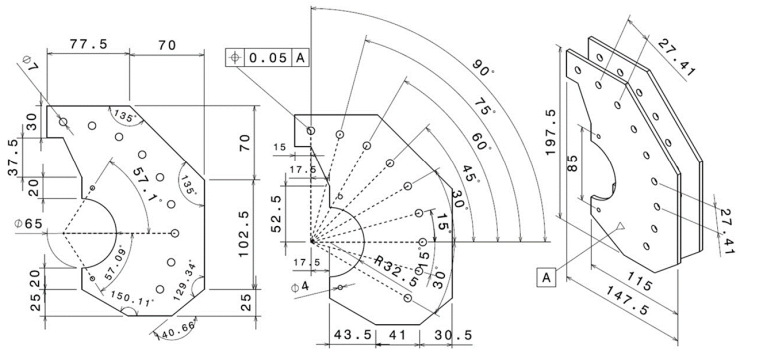
\includegraphics[width=15cm]{fig24}
	\caption{Size of the Arcan fastening system \citep{Odounga2018phd}.}
	\label{fig:fig24}
\end{figure}

The fixing holes for the wooden specimens have a diameter $\Phi= 4 mm$, and the loading holes have a diameter $\Phi = 7 mm$. These fixing holes were drilled in order to be able to load the specimen with different angular values of the angle in relation to the vertical direction in order to activate different failure modes depending on the load angle. To connect the Arcan system to the press, a piece had to be created, as shown in Figure \ref{fig:fig25}.


\begin{figure}[htp]
	\centering
	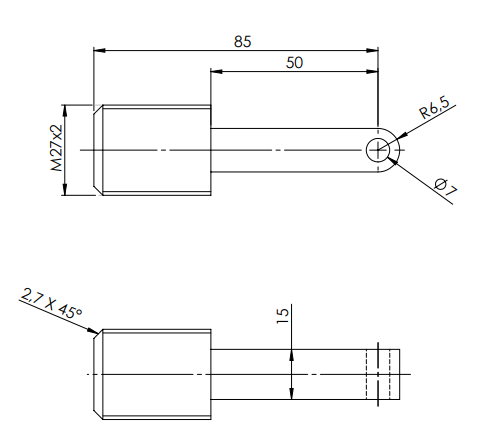
\includegraphics[width=6cm]{fig25}
	\caption{Bolt for connecting the press and the Arcan System.}
	\label{fig:fig25}
\end{figure}

This component incorporates a hole with dimensions identical to the Arcan specimen, facilitating seamless integration. Furthermore, the connector head has a diameter of 27 mm, and the thread has a pitch of 2 mm to ensure compatibility with the testing machine. The fixture was designed and assembled using SolidWorks software, and detailed technical drawings were produced for manufacturing (Figure \ref{fig:fig26}). However, before final production, a 3D printer was employed to create a prototype of the object, allowing for thorough verification and validation.

\begin{figure}[htp]
	\centering
	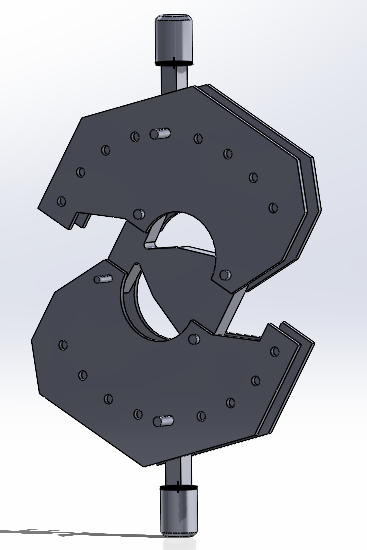
\includegraphics[width=7cm]{fig26}
	\caption{Assembled device in Solidworks.}
	\label{fig:fig26}
\end{figure}

Previous studies, including the work by \citep{Odounga2018phd}, have demonstrated a prominent issue associated with the MMCG specimen: the limited distance between the holes and the specimen extremities. This proximity leads to the formation of multiple cracks in the heel region between the hole and the sample's extremity, hindering practical observation and fracture analysis. To address this challenge, one proposed solution involves using washers that can be affixed through adhesive bonding or secured with robust screws and nuts. By applying compressive stress on each side of the sample, the stress applied to the holes is diminished, and the load is distributed across a broader area, thereby alleviating the issue.

\subsection{Universal testing machine}

The tests were conducted using a Landmark Servohydraulic Test Systems model 661.21B-03 from MTS, which served as the universal testing machine. This equipment can apply a maximum load of 100 kN (refer to Figure \ref{fig:fig27}). Displacement control was employed during the tests, with a cross-head displacement rate set to 0.1 mm/min. Data acquisition occurred at a frequency of 5 Hz. It is worth noting that in the study conducted by \citep{Mambili2018}, tests were performed at a frequency of 10 Hz, with a velocity of 0.3 mm/min and a pre-load of 100N. A pre-load was required to mount the specimen and fixture to the testing machine. However, the value of the pre-loading was considered in evaluating the energy release rate.

\begin{figure}[htp]
	\centering
	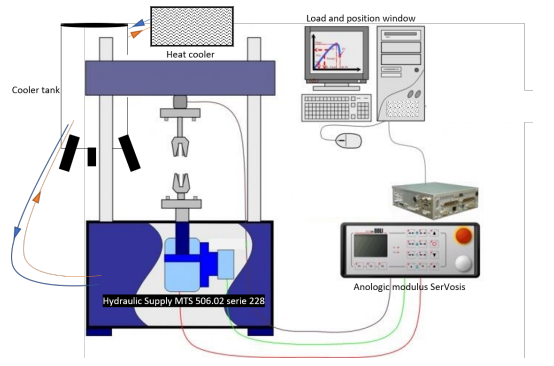
\includegraphics[width=10cm]{fig27}
	\caption{Hydraulic Press components allowing it use \citep{MALFAIT2021}.}
	\label{fig:fig27}
\end{figure}

\section{DIC method and setting parameters}

\subsection{Preparation of the DIC method}

Digital image correlation (DIC) enables the generation of displacement and strain maps, providing valuable kinematic information. The MatchID DIC 2D software was used in this study, and Python-based scripting was coded for post-processing purposes.
The focus of this study was the evaluation of crack opening displacement and crack length variation during the fracture tests with regard to the applied load. A monotonic optical system, employing a single camera, was employed. A speckle pattern was manually applied to all specimens using white-and-black spray paint to facilitate DIC analysis. The procedure involved initially applying a thin layer of white paint using a matte spray, followed by applying black paint to create a distinctive local pattern across the region of interest (ZOI) ahead of the crack tip. Notably, care was taken during lens and camera adjustments to optimise focusing and exposure time, ensuring an appropriate spread of light intensity to prevent pixel saturation in the sensor.

\subsection{MatchID}

In DIC processing, several steps are required:

\begin{itemize}
	\item Choose a reference image that corresponds to the first image of the test 
	\item Select multiple deformed images
	\item Define the zone of interest (ZOI) in which the crack propagates
	\item Define the  DIC setting parameters
	\item Start the DIC analysis
	\item Exploit the results
\end{itemize}

It is important to highlight the significant impact of both extrinsic and intrinsic setup parameters in digital image correlation (DIC), including subset size, subset step, strain gauge window, shape functions, and correlation criterion. These parameters play a crucial role in determining the calculated strain fields, resulting in variations in spatial resolution and resolution values that can differ by an order of magnitude or more \citep{DICguide2018}. The following paragraph aims to provide an explanation of some of these parameters.

\begin{itemize}
	\item The \textbf{correlation criterion} defines the matching criterion that will be adopted to determine the corresponding optimum point. In this work, ZNSSD criterion was selected. It is a least-square-based correlation criterion less sensitive to image contrast reduction and light intensity shifting between images.
	\item There are several \textbf{subset shape function} that the user can specify among rigid, affine and quadratic. Depending on the local deformation or strain gradients of the problem under analysis, the user can select affine or quadratic shape functions in the DIC method \citep{PereiraandXavier2018}.
	\item The \textbf{subset size} ($SS$) defines the spatial displacement resolution by specifying the correlation domain, that is, the number of pixels used to estimate a displacement vector. As a rule of thong, the region must contain at least three speckle light intensity variations. As an indication, larger subsets improve resolution but decrease spatial resolution. This means that in a conventional mechanical tensile test with a uniform, uniaxial stress state in the central region of the specimen, large subsets can be selected to improve the accuracy of the measurements. Nevertheless, the opposite is verified in fracture mechanics since the event of interest is relatively localised at the crack tip location.
	\item The \textbf{step size} ($ST$) refers to the amount of overlap between subset domains and determines the data points utilized in reconstructing the strain field. It plays a critical role in defining the spatial resolution of strains, meaning it controls the density of points at which DIC data is computed along a given length. Generally, setting the step size between one-third and one-half of the subset size is recommended, allowing for partial overlap between neighbouring subsets. However, it is important to note that this value can vary significantly depending on the specific application. In certain cases, a small step size may be necessary to accurately capture the peak position of a quantity of interest (QOI) within the ZOI, mainly if the QOI exhibits rapid variations without interpolation. Conversely, a larger step size can be used when the QOI changes gradually across the ZOI. The choice of step size should be carefully considered based on the specific requirements and characteristics of the investigated strain field.
	\item The \textbf{strain window} ($SW$) refers to the number of data points used to reconstruct the optimal polynomial function, using the least-square method, for calculating the analytical derivatives of strain components from the displacements. The selection of parameters such as subset size, step size, and strain window determines the spatial resolution of strain and the virtual strain gauge (VSG) characteristics.
	\item The \textbf{VSG} (virtual strain gauge) serves as a measure of spatial strain resolution and is calculated using the formula: $VSG=[(SW-1)\times ST] + SS$. The dimensions of the $VSG$ have an
    impact on the smoothness of the obtained results. Larger VSG dimensions yield smoothed results: however, the signal may be significantly underestimated in regions with heterogeneous deformation and
    significant gradients. On the other hand, a smaller $VSG$ provides data with higher noise levels but can better capture gradients. It is important to note that the pixel dimensions of the strain window are influenced by the chosen subset size and step size in the correlation algorithm. For instance, if a step size of 21 pixels is used, the availability of experimental displacement values is limited to every 21 pixels in both the horizontal and vertical directions. Consequently, an $N \times N$ strain window corresponds to a smoothing area with an actual width and height of
	[$(N-1) \times $ step size]+1 pixels. Furthermore, the displacement data points at the edges of the strain window are influenced by pixels extending beyond the dimensions. Therefore, determining strain values incorporates the subset size and should be considered accordingly.
\end{itemize}

In order to determine the most appropriate DIC settings, the Performance Analysis module within MatchID was employed. This tool allows for the definition of a range of options to be utilized in a design of experiments study. Parameters such as subset size, step size, and strain window can be varied systematically to enable a comprehensive comparison of the reconstruction of displacement and strain fields.

Subsequently, data from each analysis were extracted in a matrix format for each acquisition step. These data were then subjected to further analysis using Python scripting, with the aim of evaluating fracture parameters within the scope of this study.


\section{Python code}

Python is a widely used computer programming language renowned for its versatility and extensive range of applications. It is frequently employed in developing websites, software systems, task automation, and data analysis. Unlike some specialized programming languages, Python offers a broad scope, allowing for the creation of diverse programs to tackle various problems. Furthermore, Python's user-friendly syntax and approachable learning curve have contributed to its widespread adoption, making it one of the most popular programming languages today.

An additional data processing step is required to determine the precise position of the crack tip and calculate the corresponding crack opening displacements. This information will enable the subsequent plotting of force as a function of crack opening or crack length and the evaluation of the energy release rate ($G$) as a function of crack length ($a$). Two distinct methods for accomplishing this task will be described in the following sections.

\subsection{Method 1: Crack propagation based on full-field displacement fields provided by DIC}

\textbf{Database}

A Python database file is created to obtain information for each specimen, such as the initial crack tip, the thickness of the specimen and the chosen subset for $a_0$.

\textbf{Reading data}

The first lines of the main program consist of reading and synchronising with image acquisition, the force and the displacements of the testing machine. Moreover, DIC data in the form of a subset $X$ and $Y$ coordinates together with $U_X$ and $U_Y$ components of the displacements for each stage are also read to workspace variables.

\textbf{Crack tip opening displacement}

The Crack Tip Opening Displacement (CTOD) will be calculated by analysing subsets positioned just above and below the subset that initially defines the crack tip position ($a_0$) in the pre-crack propagation images (see Figure~\ref{fig:fig29bis}). The $a_0$ subset corresponds to a specific entry in row $m$ and column $n$ in matrix representation. Observing the subsets from top to bottom makes it possible to track the displacement of the crack tip and measure it accurately. The objective is to identify the most suitable pair of subsets sufficiently close to the crack for meaningful measurements without being too close or too far. Proximity to the crack ensures relevant information, while excessive proximity or distance may compromise the accuracy of measurements. Through the analysis of these displacements, the crack opening values at each step can be obtained.
\begin{figure}[htp]
	\centering
	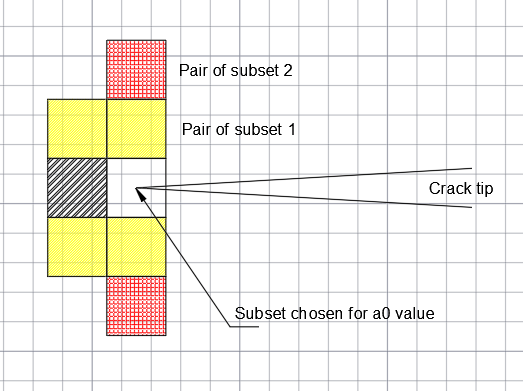
\includegraphics[width=8cm]{fig29bis}
	\caption{Pair of subsets around the chosen subset $a_0$.}
	\label{fig:fig29bis}
\end{figure}

\textbf{Mapping function and mapping mask}

The method used is based on the variation of the relative position between adjacent subsets, which gives an estimate of the damage occurrence \citep{Xavieretal2014}. To begin with, a matching function A(x,y) \ref{eq:eq21} is determined based on the norm of the relative position vectors as follows:

\begin{equation}
	A(x,y)=max(\lVert u_i-u_k\rVert;\lVert u_j-u_l\rVert)
	\label{eq:eq21}
\end{equation}

where $u_{i,j,k,l}$ represent the displacement vector of four adjacent subsets. A mapping mask is then defined, assuming threshold segmentation according to the following inequalities.

\begin{equation}
	M(x,y)=
	\begin{cases}
		1, & \text{if } A(x, y) \geq \alpha \overline{A} \\
		0, & \text{if } A(x, y) < \alpha \overline{A} \\
		-1, & \text{if } A(x, y) = \textrm{NaN}
	\end{cases}
	\label{eq:eq22}
\end{equation}

The matrix $M$ serves as the basis for estimating the current horizontal location or crack length at a given stage. Zero values in the matrix indicate areas without a crack, while subsets within the crack or regions with missing information are assigned values of 1 and -1, respectively. Subsets surrounding the crack, which are of particular interest for the study, are assigned a value of 1. Constructing a sub-matrix consisting of -1, 0, and 1, one can visualise the damage evaluation as a map, providing an overview of the crack's development. Tracking the farthest subset with a value of 1 allows the determination of the last subset where the crack tip is located. To facilitate this, the parameter $\alpha$ acts as a cutoff tool, enabling the localisation of the crack position in the matrix coordinate space.

\textbf{$\alpha$ parameter}

The selection of the $\alpha$ parameter is not straightforward in the initial approach. To approximate its value, we first seek a correlation factor using the least squares regression method. During the test, the load-displacement curve consists of three main regions: a linear region representing a stationary zone, a second region corresponding to fracture propagation, and a third region indicating specimen rupture. By determining the correlation factor, we can identify the stage between the stationary zone and the Fracture Process Zone (FPZ). A second verification criterion based on displacement field processing is then applied to confirm the correct stage of the FPZ. By following these two steps, we can determine the stage at which the FPZ begins and the possible range of values for $\alpha$. Subsequently, we can plot the stages of crack propagation for different $\alpha$ values and assess the value of $\alpha$ that yields the largest $a(t)$ (crack length). Typically, the smallest $\alpha$ is chosen, unless a curve with simpler geometry is desired and the length of $a(t)$ remains relatively unchanged. A portion of the code enables graphical verification of the crack length by directly selecting $a_0$ and $a_f$ in Python. This allows the elimination of certain $\alpha$ values that do not yield the correct crack length.

\textbf{Crack length}

Another section of the code focuses on obtaining $a(t)$ as a function of $\alpha$. This is achieved by examining the ZOI and the subsets within it. By analysing the displacement field derived from each subset, the code calculates the distance between the centre of a subset and its displacement from one image to another. To simplify the code, this calculation is performed only on the four corner subsets. By measuring the distance between opposite corners, we obtain the maximum displacement in the $x$-direction and the displacement in the $y$-direction, which are then incorporated into a final matrix. Subsequently, the value of $a(t)$ is determined. It is equal to the initial crack length, $a_0$, specified by the user in the database, plus $\Delta a$, which represents the crack length variation over time in response to the applied force.


\subsection{Method 2: Crack propagation based on crack opening displacement provided by DIC}

Method 2 uses the crack opening along the entire length of the wooden specimen to determine the length of the crack \citep{FilhoJ2022}.

\textbf{Crack opening displacement (COD) or Virtual displacement}

From the reference and current positions of the DIC calculation points, the Euclidean distance between each pair of points can be measured and the COD can be determined as:

\begin{equation}
	VD(k,i_n)=\sqrt{(x_{11bk}-x_{11tk})^2 + (x_{22bk}-x_{22tk})^2}_{i_n} - VD(k,i_0)
	\label{eq:eq23}
\end{equation}

where the indices $t$ and $b$ refer to the DIC data points located at the top and bottom of the crack path, $k$ is the index of the DIC point, $i_n$ is the image captured at time $n$, $VD(k, i_0)$ is the initial Euclidean distance between the computational points of the top and bottom reference DIC subset obtained from image $i_0$, and $x_{11}$ and $x_{22}$ are their coordinates in the image plane. VD can be defined as a displacement gauge along the crack path \ref{fig:fig30}.

\begin{figure}[htp]
	\centering
	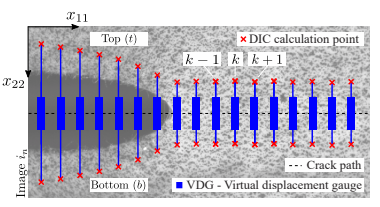
\includegraphics[width=10cm]{fig30}
	\caption{DIC-based virtual displacement gauge (VDG) \citep{FilhoJ2022}.}
	\label{fig:fig30}
\end{figure}

\textbf{$\alpha$ and $\beta$ parameters}

The first step towards detecting the crack tip is to take the average value of $VD$ for each stage:

\begin{equation}
	\overline{VD}(i_n)=\frac{1}{k} \sum_{k=1}^{k}VD(k,i_n)
	\label{eq:eq24}
\end{equation}

The threshold value must be adjusted using the two parameters $\alpha$ and $\beta$ which are obtained by solving the equation:

\begin{equation}
	\begin{cases}
		VD_{th}(i_1)=\overline{VD}(i_1)(\alpha i_1 +\beta)\\
		VD_{th}(i_f)=\overline{VD}(i_f)(\alpha i_f +\beta)\\ 
	\end{cases}
\label{eq:eq25}
\end{equation}

In order to obtain $VD_{th}(i_1)$ and $VD_{th}(i_f)$, it was first necessary to read graphically the position of the crack tip of the first and last image and then to find the intersection between the position of the crack tip and the crack opening VD for those two stages.

Therefore, the adjusted threshold line-cut $VD_{th}(i_n)$ is given by:

\begin{equation}
	VD_{th}(i_n)=\overline{VD}(i_n)(\alpha i_n +\beta)
	\label{eq:eq26}
\end{equation}

The intersection between each $VD_{th}(i_n)$ and the corresponding $VD(k, i_n)$ curve at time n represents the $x_{11}$ position of the crack tip, denoted by ($p_n$).
It is therefore possible to calculate the growth of the crack at instant $n$:

\begin{equation}
	da_n=p_n-p_0
	\label{eq:eq27}
\end{equation}

\subsection{Difficulties in applying method 2}

This method was originally used for a fibrous soft material. The first step was to translate the Matlab code given by \citep{FilhoJ2022} into a python code to be able to use both methods simultaneously and compare them.
After translating the code, we realised that this method did not work properly for the wood material and the DIC data from prelinary MMCG tests~\citep{MALFAIT2021}.
From the data of method 1, we already know the position of $a_0$ and all the displacements over time that have occurred on the entire wooden specimen. However, for method 2, we only need 2 horizontal lines placed above and below the fracture. It is therefore sufficient to take only one part of the data from the specimen. Moreover, it was chosen to take these two lines far enough away from the fracture in order not to have subsets without any data. However, method 2 still didn't work properly and a slight modification to the code was required.

The Figure \ref{fig:fig31} corresponds to the plot of $\overline{VD}$ and $VD_{th}$ with Joao's data. We read graphically $a_1$ and $a_f$, which allowed us to know the $VD_{th}$ for index 1 and the last index which are the bounds on the y-axis for the $VD_{th}$ curve. We notice that the $VD_{th}$ curve has the same shape as the $\overline{VD}$ curve, is still increasing but has only been reduced at the ordinate level. This is what we want to achieve for the MMCG specimens.

For the MMCG test data, by applying $VD_{th1}$ and $VD_{thf}$ as in Joao's data, we notice that the $VD_{th}$ curve increases and then decreases, which is not normal since the COD should normally increase with time (figure \ref{fig:fig32}). This is due to the alpha and beta factors which increase $\overline{VD}$ for the first indices and then decrease $\overline{VD}$ for the last indices. According to the equation \ref{eq:eq26} alpha is multiplied by $i_n$ which will decrease the multiplier coefficient of $\overline{VD}$ over time if alpha is negative and beta positive. This is the reason why $VD_{th}$ is under $\overline{VD}$  for the latest indices.

\begin{figure}[htp]
	\begin{minipage}[c]{.46\linewidth}
		\centering
		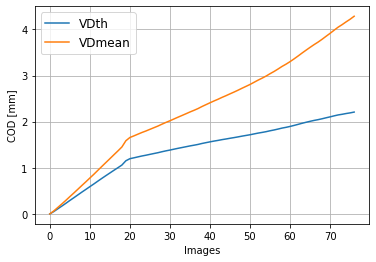
\includegraphics[width=7cm]{fig31}
		\caption{$\overline{VD}$ and $VD_{th}$ with Joao's data.}
		\label{fig:fig31}
	\end{minipage}
	\hfill%
	\begin{minipage}[c]{.46\linewidth}
		\centering
		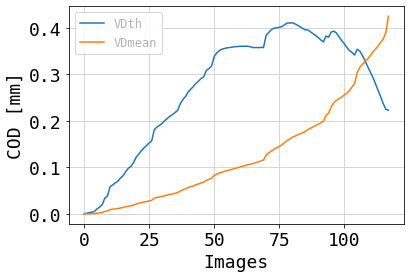
\includegraphics[width=7cm]{fig32}
		\caption{$\overline{VD}$ and $VD_{th}$ with stanislas' data.}
		\label{fig:fig32}
	\end{minipage}
\end{figure}


Method 1 was then used to find out from which image the fracture process starts. Method 2 directly increased the length of the crack for the first images, which is not normally the case for wood.  Indeed, it is considered that for all the images before the FPZ there is a(t)=a0. We therefore read $a_1$ and $a_f$ with $a_1$ the index of the beginning of the fracture process and $a_f$ the last image before the material breaks. The Figure~\ref{fig:fig33} is then obtained.


\begin{figure}[htp]
	\centering
	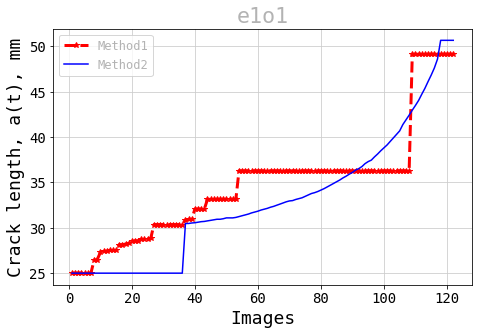
\includegraphics[width=7cm]{fig33}
	\caption{Crack length with FPZ taken into account.}
	\label{fig:fig33}
\end{figure}

The fracture for method 2 starts much later than method 1 and are different over the time. Furthermore, the crack length does not end at the same place, because for method 2 the fracture at the last index is read graphically which is less accurate.
Because the $\overline{VD}$ is too small compared to the graphically obtained $VD_{th1}$, an interpolation is made to increase the $\overline{VD}$. The Figure \ref{fig:fig34} is obtained:

\begin{figure}[htp]
	\centering
	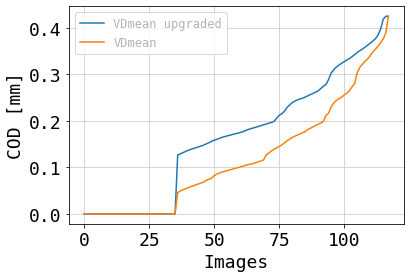
\includegraphics[width=7cm]{fig34}
	\caption{Interpolation of $\overline{VD}$.}
	\label{fig:fig34}
\end{figure}

Thanks to this interpolation, we apply alpha and beta (figure \ref{fig:fig35}) and obtain $VD_{th}$. Finally, we obtain the crack length Figure \ref{fig:fig36}:

\begin{figure}[h]
	\begin{minipage}[c]{.46\linewidth}
		\centering
		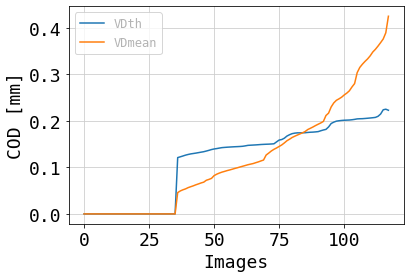
\includegraphics[width=7cm]{fig35}
		\caption{$VD_{th}$ with interpolation.}
		\label{fig:fig35}
	\end{minipage}
	\hfill%
	\begin{minipage}[c]{.46\linewidth}
		\centering
		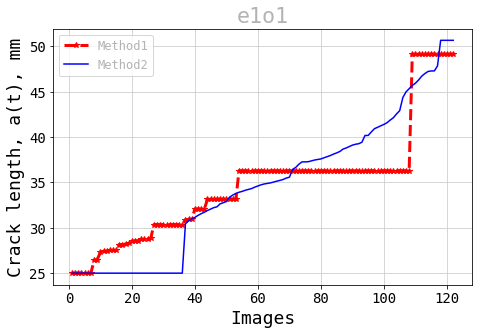
\includegraphics[width=7cm]{fig36}
		\caption{Final crack length e1o1.}
		\label{fig:fig36}
	\end{minipage}
\end{figure}

To conclude, the crack propagation does not start at the same stage between the two methods and the crack length is different over the time. Moreover we had to modify a lot Joao's initial method to apply it to wood material. It also adds uncertainties since we have to read graphically $a_1$ and $a_f$ to obtain the crack length thresholds at the beginning and at the end of the propagation. Reading the points $a_1$ and $a_f$ is really difficult to evaluate manually for this material because the fracture is not clearly visible on the images. In addition, the index for $a_1$ and $a_f$ is given by method 1 which adds further uncertainties. Method 2 gives a "smoother" curve than method 1, but this is not necessarily a good thing since the fracture of wood material usually works in fits and starts.
As observed in method 1, the fracture process typically involves multiple stages, which can be attributed to the gradual propagation of cracks. In some instances, the presence of bridges in the material can impede the linear advancement of the crack. However, once these bridges break, the crack can propagate further, resulting in the development of a new stage in the fracture process. This underscores the complex nature of crack propagation in wood. In the next chapter, the tests carried out in mode I will be presented and we will be able to check whether method 2 works correctly with wood. However, some doubts are raised, as the $\overline{VD}$ is not as linear as with a soft fibrous material, as shown in Figures \ref{fig:fig31} and \ref{fig:fig32}.

\subsection{Energy release rate}

After using one of the two previous methods, we can calculate the energy release rate in mode I and in mixed mode I+II. For mode I, the formula is the one explained in \ref{eq:eq125}. For mixed mode I+II, the formula is given as:

\begin{equation}
	\begin{cases}
		G_\text{I}=\displaystyle\frac{{F_{cy}}^2}{2b}\ \frac{\partial C_\text{I}}{\partial a} \quad \text{with } C_\text{I}=\frac{v}{F_{cy}} \\
		G_\text{II}=\displaystyle\frac{{F_{cx}}^2}{2b}\ \frac{\partial C_\text{II}}{\partial a} \quad \text{with } C_\text{II}=\frac{u}{F_{cx}}\\
	\end{cases}
\label{eq:eq28}
\end{equation}

where $u$ and $v$ are the crack opening displacement according to $x$ and $y$. The displacement measured by the machine is not used to calculate the energy release rate, as it is less accurate due to the clearances in the jaws.

Using the Arcan fixture, the mixed mode I+II fractur loading is achieved by rotating the fixture with regard to the testing machine. Accordingly, the camera-lens optical system will be also rorated with regard to the specimen as shown in Figure \ref{fig:fig37bis}.

\begin{figure}[htp]
	\centering
	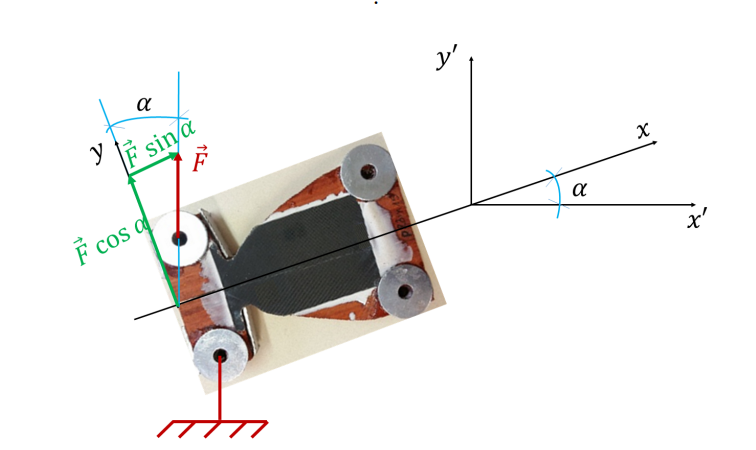
\includegraphics[width=.7\textwidth]{fig37bis}
	\caption{Force projection along the axes in mixed mode, \citep{Odounga2018phd}.}
	\label{fig:fig37bis}
\end{figure}

The crack opening values will therefore be projected directly along the $x$ and $y$ axes.
Accordingly, the force is also projected along the $x$ and $y$ axes as:


\begin{equation}
	\begin{cases}
		F_{cx}=F \sin(\alpha) \\
		F_{cy}=F \cos(\alpha) \\ 
	\end{cases}
	\label{eq:eq29}
\end{equation}

\noindent where $\alpha$ represents the angle between the vertical axis and local vertical orientation of Arcan specimen (Figure \ref{fig:fig37bis}).

\section{Specimen preparation}

\subsection{Specimen names}

We have 20 specimens of silver fir with a thickness of 12.5mm. We will use five specimens per degree of inclination to investigate different fracture modes. This means five specimens in pure mode I (0°) and 15 specimens in mixed mode (15°, 30°, and 45°).
Naming the specimens allows us to identify which test was performed on each specimen. The first part of the name corresponds to the inclination of the specimen during the test using the Arcan system:

\begin{itemize}
	\item E0: Test in pure mode I;
	\item E15: Test with a specimen tilt of 15°;
	\item E30: Test with a specimen tilt of 30°;
	\item E45: Test with a specimen tilt of 45°.
\end{itemize}

Therefore, E15, E30, and E45 are the specimens tested in mixed mode. The second component of the name represents the number of the specimen dedicated to that specific test. Finally, all samples are named as E0E1, which is the first sample used in pure mode.

\subsection{Notch and precrack}

Notches were created in each specimen to initiate a sharp, straight crack. A pre-crack was made using a cutter at the notch, ensuring that it was centred at the heel of the sample. The notch width was 1.5 mm, created using a straight electrical saw. Using a cutter allowed precise control over the pre-crack shape, enabling proper crack propagation. The notch on each side of the specimen and the pre-crack were measured and averaged to determine the initial crack length. The initial crack length is denoted as $a_i$, and the total crack length is given by $a = a_i + \Delta a$, where $\Delta a$ represents the crack growth.
The initial crack lengths for each specimen are summarized in Table~\ref{tab:Tab11}. It is important to note that only one test was conducted at a 45-degree angle, while multiple tests were performed for angles 0°, 15°, and 30°. Some tests were unsuccessful, so the focus was placed on the tests carried out at 0°, 15°, and 30° angles.

\begin{table}[h]
	\centering
	\begin{tabular}{m{.1\textwidth} m{.2\textwidth}}\toprule
		\multicolumn{1}{l}{} & \multicolumn{1}{l}{Initial Crack length} \\\midrule
		\multicolumn{1}{c}{\cellcolor[HTML]{F8CBAD}E0E1} & 25,3   mm \\
		\multicolumn{1}{c}{\cellcolor[HTML]{F8CBAD}E0E2} & 24.85 mm \\
		\multicolumn{1}{c}{\cellcolor[HTML]{F8CBAD}E0E3} & 25.65 mm \\
		\multicolumn{1}{c}{\cellcolor[HTML]{F8CBAD}E0E4} & 24,7 mm \\
		\multicolumn{1}{c}{\cellcolor[HTML]{F8CBAD}E0E5} & 25,6 mm \\
		\multicolumn{1}{c}{\cellcolor[HTML]{F8CBAD}E0E6} & 26,3 mm \\
		\multicolumn{1}{c}{\cellcolor[HTML]{C65911}E15E1} & 25,85 mm \\ 
		\multicolumn{1}{c}{\cellcolor[HTML]{C65911}E15E2} & 25,6 mm \\ 
		\multicolumn{1}{c}{\cellcolor[HTML]{C65911}E15E3} & 25,55 mm \\ 
		\multicolumn{1}{c}{\cellcolor[HTML]{C65911}E15E4} & 25.3 mm \\
		\multicolumn{1}{c}{\cellcolor[HTML]{C65911}E15E5} & 24,85 mm \\ 
		\multicolumn{1}{c}{\cellcolor[HTML]{BF8F00}E30E1} & 25,55 mm \\ 
		\multicolumn{1}{c}{\cellcolor[HTML]{BF8F00}E30E2} & 24,4 mm \\ 
		\multicolumn{1}{c}{\cellcolor[HTML]{BF8F00}E30E3} & 24,2 mm \\ 
		\multicolumn{1}{c}{\cellcolor[HTML]{BF8F00}E30E4} & 25,3 mm \\ 
		\multicolumn{1}{c}{\cellcolor[HTML]{BF8F00}E30E5} & 24.4 mm \\ 
		\multicolumn{1}{c}{\cellcolor[HTML]{BF8F00}E30E6} & 24.35 mm \\ 
		\multicolumn{1}{c}{\cellcolor[HTML]{BF8F00}E30E7} & 25.6 mm \\
		\multicolumn{1}{c}{\cellcolor[HTML]{FFA500}E45E1} & 25,8 mm \\ 
		\multicolumn{1}{c}{\cellcolor[HTML]{00FF00}broken} & 25.95 mm \\\bottomrule
	\end{tabular}
	\caption{Precrack dimensions.}
	\label{tab:Tab11}
\end{table}

\section{Conclusion}

This chapter comprehensively explains the materials and methods developed for fracture tests. It has also elucidated key parameters crucial for successfully implementing the DIC method. Furthermore, two distinct approaches for assessing crack length were presented: one based on full-field displacement analysis and the other on COD measurements.
Based on the results obtained from both methods, method 1 exhibits higher accuracy than method 2. In the subsequent chapter, a more comprehensive evaluation of the effectiveness of these two methods will be conducted, allowing for a more conclusive assessment of their efficiency.


%\chapter{Experimental work and results in mode I}
\label{Chapter3}

\section{Introduction}

This chapter outlines the experimental work to investigate mode I fracture using MMCG specimens using the DIC method. Firstly, the experimental set-up is described in detail. Subsequently, the mode I results are presented, and the energy release rates for mode I MMCG samples are calculated and discussed in relation to existing literature.

\section{Experimental set-up}

The fracture tests were performed using a Landmark Servohydraulic testing machine with a maximum capacity of 100 kN. Figure~\ref{fig:Setup0°} shows the experimental set-up, which includes the Arcan fixture and the optical camera-lens-illumination devices. The Arcan fixture was mounted to the testing machine using standard bolts, with washers inserted between the specimen and the Arcan system to reinforce the attachment points. To facilitate specimen changes between tests, manual controls were employed to elevate the moving part of the testing machine, minimising residual tension between the bolt holes and the Arcan system. Furthermore, before testing, an arbitrary pre-load was applied to the specimen to prevent any clearance or unintended movement of the specimen (which could cause image defocusing). Load and cross-head displacement data were recorded at a frequency of 5 Hz . Additionally, a real-time plot was generated during the test for visualisation.


An Alvium 1800 U-2040m Allied Vision camera and a 60 mm Nikkor lens were used for image grabbing and acquisition. The camera has a resolution of 4512 (H) $\times$ 4512 (V) and a sensor size of type 1.1. The front of the lens was positioned at a working distance of 285 mm with an aperture of f/11 and an exposure time of 60 milliseconds. The cross-head displacement of the testing machine was 0.02mm/s, and the camera had a frequency of 1 Hz (1 fps).
 A green illumination set-up was used to enhance the sensitivity of the sensor. The camera was securely mounted on a tripod to ensure a stable position relative to the specimen's target surface, enabling the capture of consistent images throughout the tests. The frontal face of the specimens was coated with a suitable speckle pattern. A first layer of white paint was added and a cloud of black dots formed a second layer of paint. Figure~\ref{fig:Speckle_DIC} shows an image of the speckle pattern, along with its corresponding image histogram. Additionally, a scale positioned in the surface plane was employed to establish the conversion factor for translating pixels into millimetres.


\begin{figure}[htp]
	\centering
	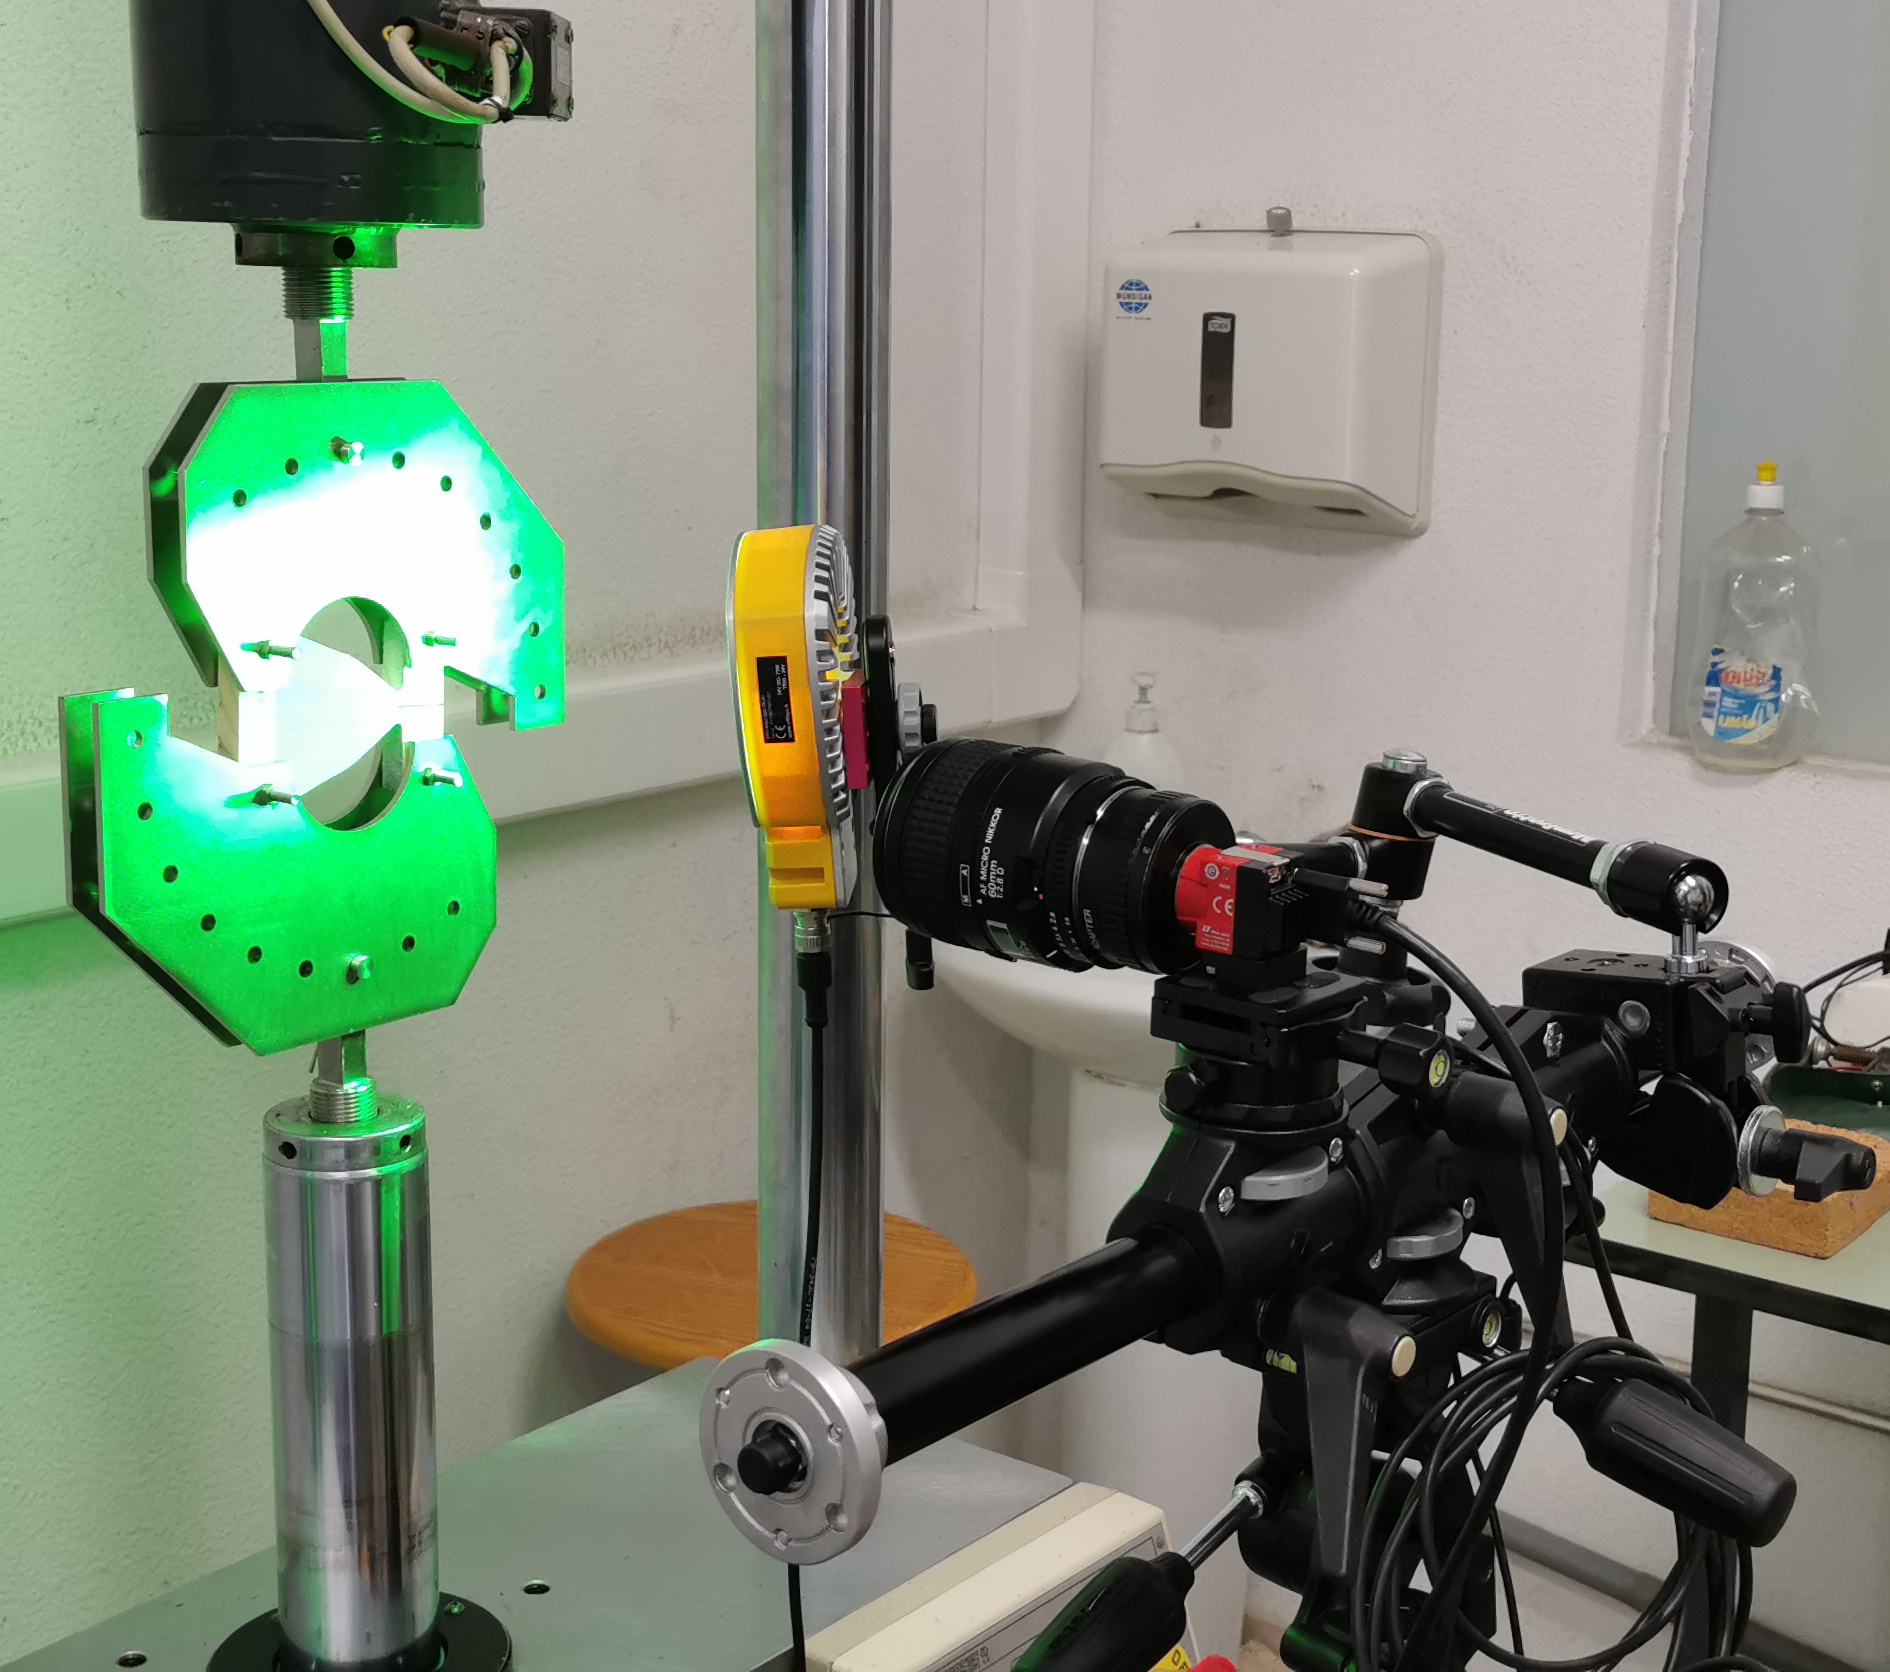
\includegraphics[width=.6\textwidth]{Setup0_crop}
	\caption{Experimental set-up.}
	\label{fig:Setup0°}
\end{figure}


\begin{figure}[htp]
	\centering
	\begin{tabular}{c}
		\includegraphics[width=5cm]{Speckle_DIC} \\
		(a) \\
		\\
		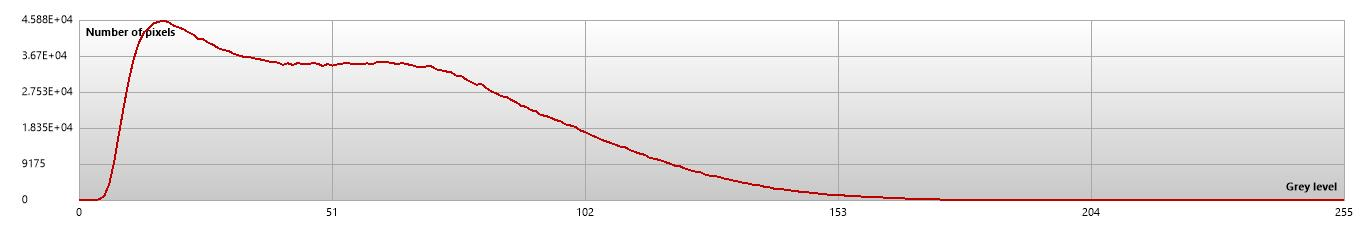
\includegraphics[width=16cm]{histogram} \\
		(b) \\
		\\
	\end{tabular}
	\caption{(a) Speckle pattern typically obtained with DIC; (b) Histogram of the speckle image.}
	\label{fig:Speckle_DIC}
\end{figure}


The selected parameters for the DIC analysis play a crucial role in determining the accuracy and spatial resolution of the measured displacements and reconstructed strain fields \citep{Xavier2012207,PereiraandXavier2018}. Consequently, they are considered fundamental factors. To achieve a trade-off between spatial resolution and accuracy, a parametric analysis was conducted utilizing the Parametric Module of MatchID. The resulting DIC settings are summarized in Table~\ref{tab:MatchID_param}.

The range of values defined in this performance study, including the subset size ($f_s$), subset step, affine and quadratic displacement shape functions, the size of the strain windows, and the order of the polynomial fitting function, is defined by the table \ref{tab:MatchID_param}. It is believed that the pre-selected range of values is reflective of the permissible DIC setup parameter range.

\begin{table}[]
	\centering
	\begin{tabular}{m{.3\textwidth}m{.4\textwidth}}\toprule
		Correlation   Coefficient: & ZNCC \\
		Interpolation order: & Bicubic Splines \\ 
		Transformation order: & Quadratic \\
		Prefiltering: & Gaussian \\
		Progress history: & Spatial \\
		Subset size: & 31 \\
		Step size: & 10 \\
		Strainwindow size: & 5 \\ 
		Virtual Strain Gauge: & 71 pixel \\
		Strain interpolation: & bilinear (Q4) Lagrange polynomials\\
		Strain Convention: & Green-Lagrange \\\bottomrule
	\end{tabular}
	\caption{DIC setting parameters used in the MatchID software for the analyses.}
	\label{tab:MatchID_param}
\end{table}


\section{Results and comparison in mode I}

\subsection{Load-displacement curves}

Normally four distinct parts are observed on a load-displacement curve for Mode I fracture loading:

\begin{itemize}
	\item A small area visible at the beginning of the curve which corresponds to the setting up of the loaded specimen. 
	\item A nearly linear region arises from the elastic loading phase with a static crack front.
	\item The third segment is distinguished by a series of critical force peaks, which signify a distinct crack initiation. The progressive increase in these peaks confirms the crack's stability zone.
	\item Lastly, the final segment entails the material's rupture, which transpires when an ultimate force is applied, marking the instability of the crack.
\end{itemize}

Because of the preload applied at the fixture and specimen adjustments, the raw load and displacements were slightly shifted to reproduce the initial conditions of zero displacements and load at the reference configuration. This extrapolation is possible because the curve has an initial linear regime. All load-displacement curves are summarised in appendix \ref{Appendix1}.


\begin{figure}[htp]
	\begin{minipage}[c]{.46\linewidth}
		\centering
		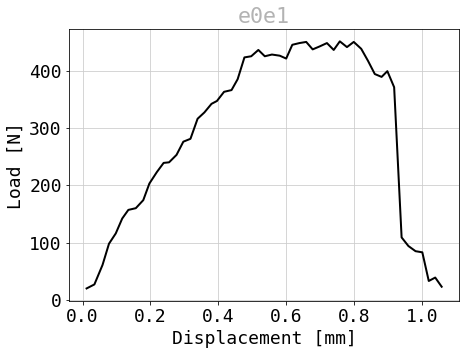
\includegraphics[width=8cm]{P_e0e1}
		\caption{Characteristic load-displacement ($P-\delta$) curve.}
		\label{fig:e0e1_Pdelta}
	\end{minipage}
	\hfill%
	\begin{minipage}[c]{.46\linewidth}
		\centering
		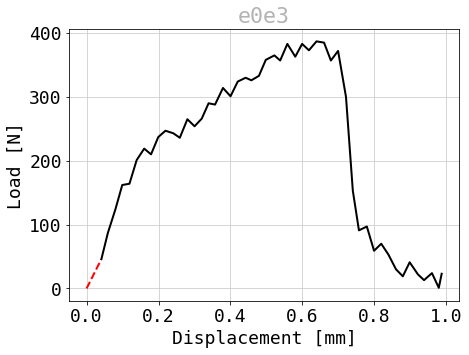
\includegraphics[width=8cm]{P_e0e3}
		\caption{load-displacement ($P-\delta$) curve shifted.}
		\label{fig:e0e5_Pdelta}
	\end{minipage}
\end{figure}


\subsection{Deformation fields}

Typical $y$-component of the strain field ($\epsilon$yy) obtained with the DIC method is shown in Figure \ref{fig:Strain_def}.
During the tests we noticed that the cracks tend to propagate according to the orientation and inclination of the grain, as expected.
In Figure \ref{fig:Strain_def} for specimen e0e1, we assume a small fibre inclination which could explain the observed crack orientation.

\begin{figure}[htp]
	\centering
	\begin{tabular}{c}
		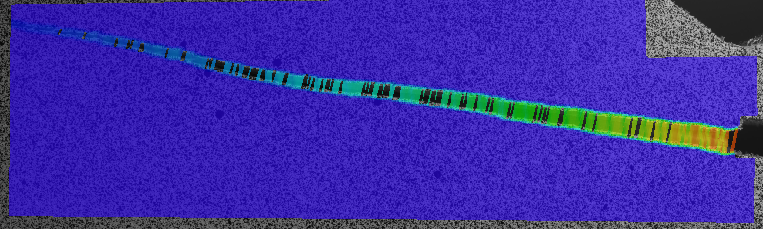
\includegraphics[width=8cm]{e0e1} \\
		e0e1 deformation map \\
		\\
		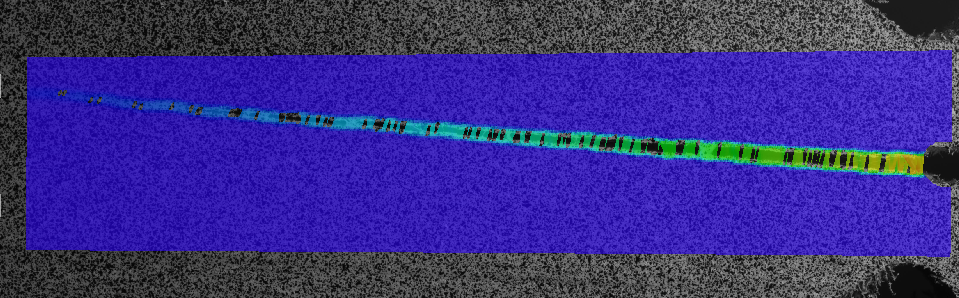
\includegraphics[width=8cm]{e0e2} \\
		e0e2 deformation map \\
		\\
		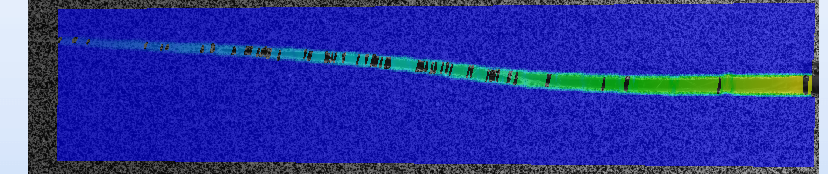
\includegraphics[width=9cm]{e0e3} \\
		e0e3 deformation map \\
	\end{tabular}
	\caption{Typical deformation map ($\epsilon_{yy}$) obtained with DIC.}
	\label{fig:Strain_def}
\end{figure}

Strain maps are employed to track the position of the crack tip at a macroscopic level during the tests. This analysis serves to validate the crack tip position obtained through both the proposed methods 1 and 2. The blue data points in Figures \ref{fig:fig39} and \ref{fig:fig40} correspond to tests e0e2 and e0e3, respectively, and are obtained through graphical interpretation of the $\varepsilon_{yy}$ strain fields. It is evident that the blue points align accurately with the curves generated by method 1, indicating the consistency of this approach. While method 2 appears to have slightly lower accuracy, we will still employ it to determine $G$ and assess the impact of minor variations in $a(t)$.

\begin{figure}[htp]
	\begin{minipage}[c]{.46\linewidth}
		\centering
		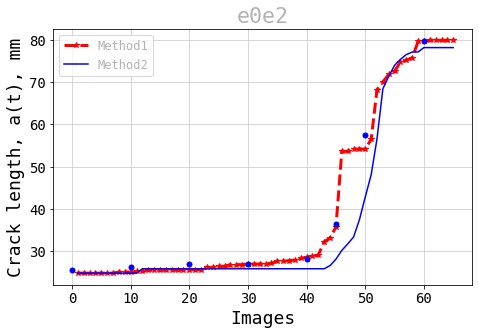
\includegraphics[width=8cm]{e0e2_graphicread}
		\caption{Crack tip by graphic reading e0e2.}
		\label{fig:fig39}
	\end{minipage}
	\hfill%
	\begin{minipage}[c]{.46\linewidth}
		\centering
		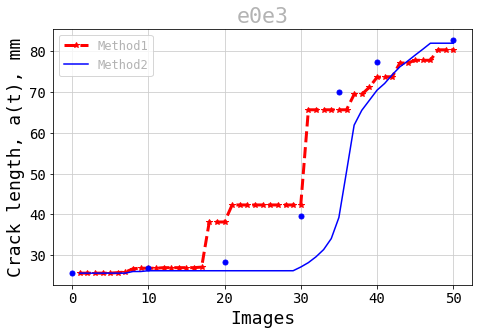
\includegraphics[width=8cm]{e0e3_graphicread}
		\caption{Crack tip by graphic reading e0e3.}
		\label{fig:fig40}
	\end{minipage}
\end{figure}


\subsection{Crack tip opening curves}

The user is required to select a pair of subsets for evaluating CTOD. To ensure precise displacement measurement, the chosen subsets must be positioned as close to the crack tip as possible while avoiding the borders and edges of the new crack surfaces. Based on this study, the databases are updated using the selected COD pair. To visually represent the selected CTOD, a plot was generated, as shown in Figure \ref{fig:CTOD_example}, with the chosen CTOD pair highlighted in blue. Additionally, to demonstrate the utmost precision of the selected COD pair for each specimen, the plot includes a comparison with the curve obtained using the lower and upper COD pairs.

\begin{figure}[htp]
	\centering
	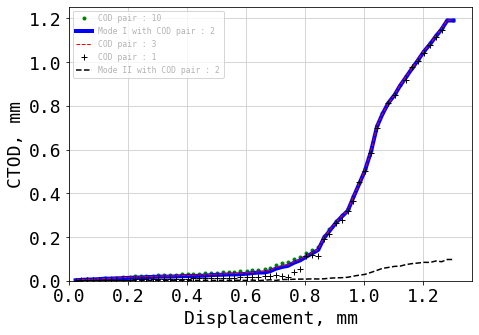
\includegraphics[width=9cm]{CTOD_example}
	\caption{Crack Tip Opening Displacement choice.}
	\label{fig:CTOD_example}
\end{figure}

Figure \ref{fig:COD_modeI} shows the crack opening curves in mode I, representing the displacement of the two surfaces of the crack. These curves exhibit two distinct phases. Initially, there is a phase where the force increases slightly alongside a minor CTOD increment. Subsequently, a second phase follows, characterised by a decrease in load and a rapid CTOD increase. During the first phase, the MMCG specimen effectively withstands the force exerted by the tensile machine, while in the second phase, the crack is already propagating. Consequently, the wood sample offers minimal resistance, leading to a notable force reduction and a significant CTOD increase.
For calculating $G$, only the section of the curve preceding the abrupt decrease in force, denoted as $P$, will be utilised. Taking curve e0e6 as an example, it is observed that the specimen fractures at a CTOD of approximately 1.2 mm, prompted by a sudden decline in force.

\begin{figure}[htp]
	\centering
	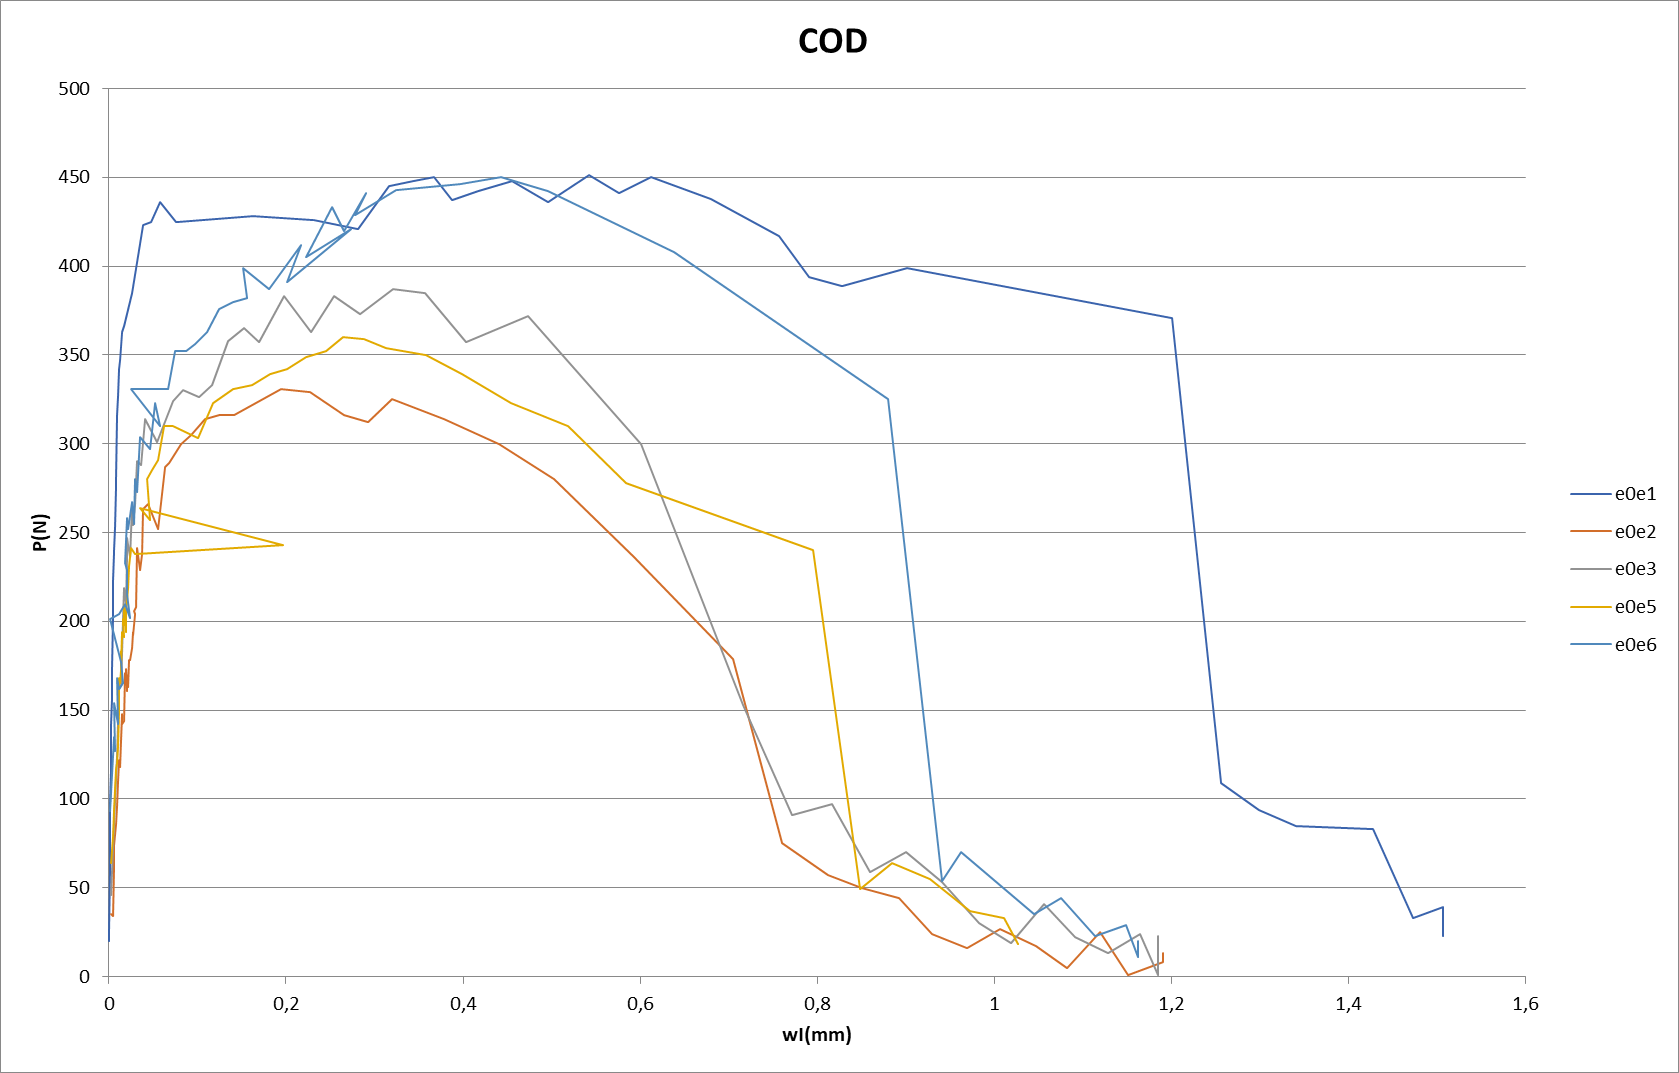
\includegraphics[width=13cm]{COD_modeI}
	\caption{Crack Tip Opening Displacement.}
	\label{fig:COD_modeI}
\end{figure}

\subsection{Crack length curves}

For method 1 by compiling the evolution of $a(t)$ as a function of the images recorded for several $\alpha$ values (\ref{fig:Cracklength_modeI_example}), it is possible to get an idea of the $\alpha$ value required to obtain the best $a(t)$. Indeed, the $\alpha$ parameter must be as small as possible for the evolution of the crack length to be complete. So, for each crack length in the sample, it is possible to eliminate several candidates. In this example \ref{fig:Cracklength_modeI_example}, it is possible to eliminate the use of curves with $a(t)<70$ mm. These $\alpha$ values do not allow the entire crack length to be studied. To distinguish between the black and turquoise curves, you can place the position of the crack tip with a red dot on the displacement map. Then for different stages, we can then see which curve corresponds best to the position of the crack tip. Here, the black curve was chosen.

To obtain $a(t)$ using method 2, we need to read $a_1$ and $a_f$ graphically and choose a pair of COD lines that are not damaged by nans values.

\begin{figure}[H]
	\centering
	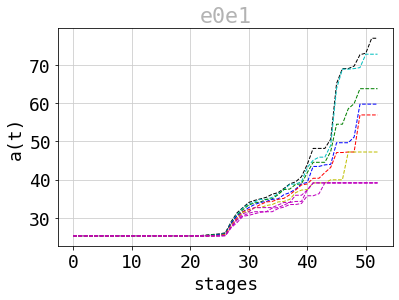
\includegraphics[width=9cm]{Cracklength_modeI_example}
	\caption{Crack length evolution depending on alpha.}
	\label{fig:Cracklength_modeI_example}
\end{figure}

Figure \ref{fig:crack_method1} and \ref{fig:crack_method2} present all the crack length curves corresponding to mode I displacement. In method 1, the expected presence of distinct plateaus in the crack length is observed. The crack length progressively and continuously increases before reaching rupture. The design of the MMCG specimen facilitates stable crack propagation, where cracks propagate slowly until failure occurs at maximum load. Some images show bridges defining a damaged fracture process zone. Extending the crack from these fibre bridging allows for continuous crack propagation. Analysing all the crack length propagation plots is interesting. The curves exhibit similar shapes, and the crack ends at approximately the same length. The variation lies in the stage at which crack propagation initiates. For example, in method 1, e0e1 begins crack propagation at stage 23, whereas e0e2 starts at stage 9.

In contrast, method 2 yields similar curves to method 1, but they appear smoother. However, this smoothness is not necessarily advantageous as crack propagation in wood typically occurs in a more step-by-step manner. Furthermore, upon checking Figure \ref{fig:a_e0e1} or Figure \ref{fig:a_e0e2} in the appendix, it can be observed that the crack length in method 2 is generally smaller than that in method 1 for the same stage.

\begin{figure}[htp]
	\centering
	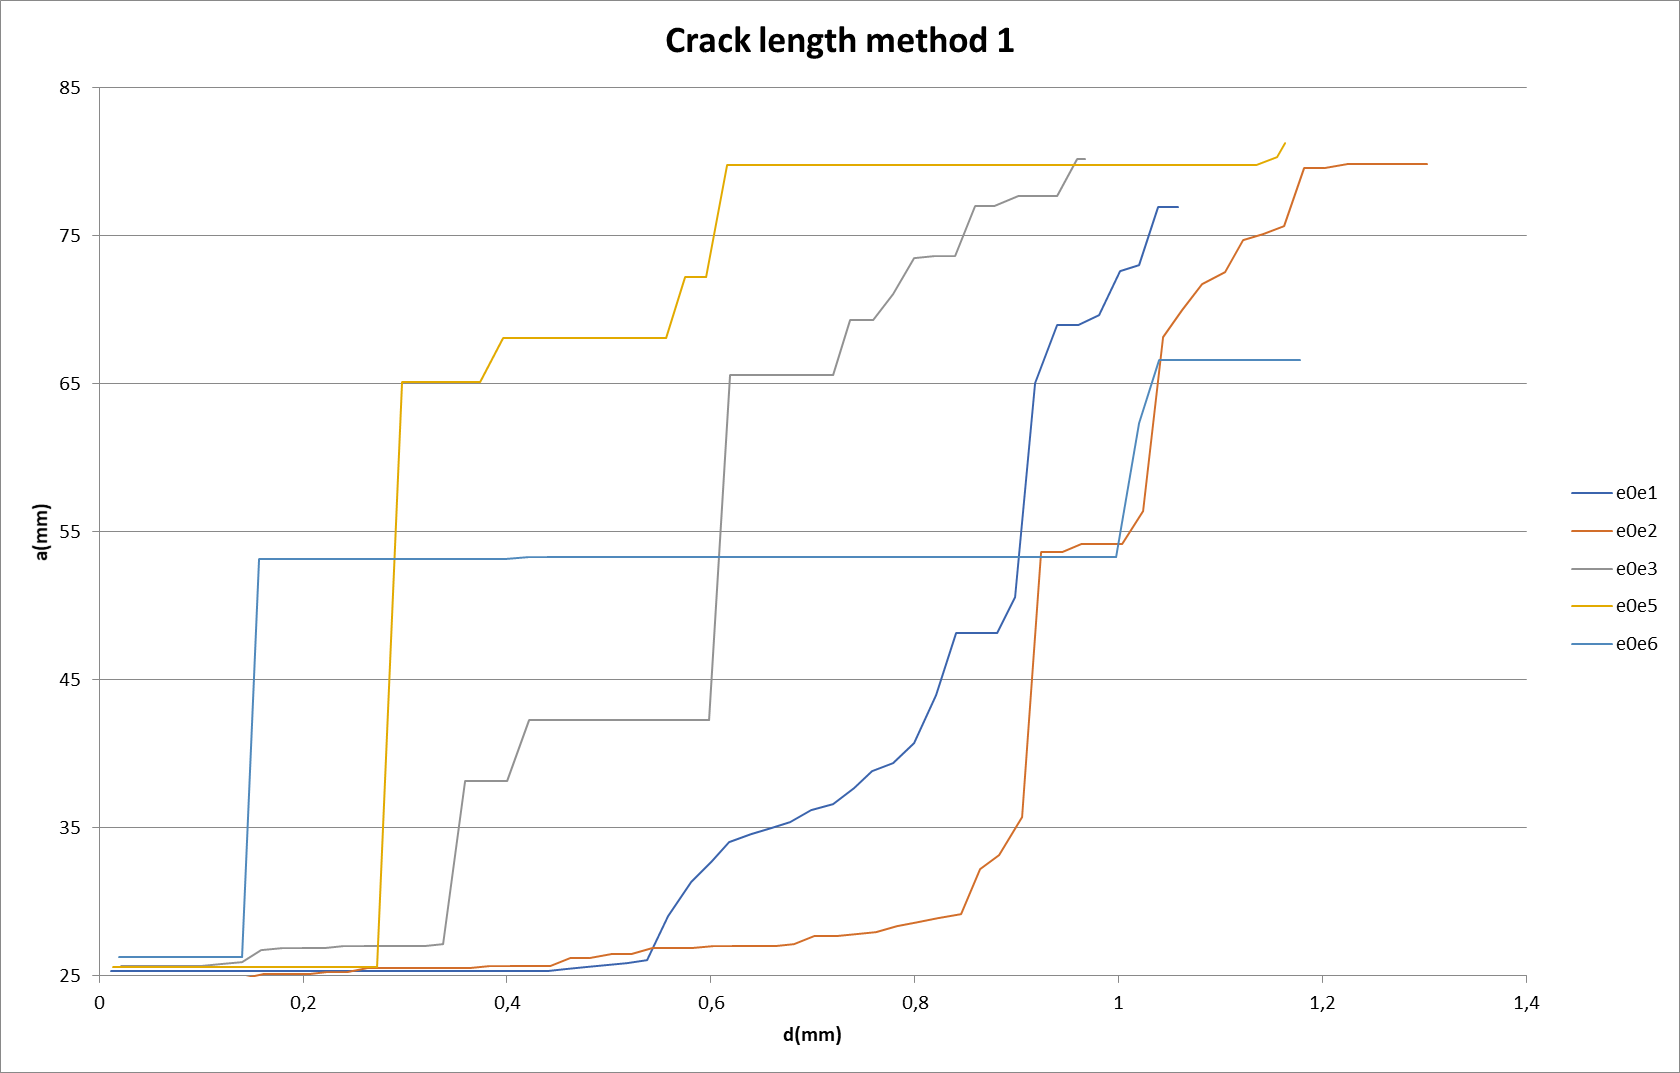
\includegraphics[width=13cm]{crack_method1}
	\caption{Crack length evolution method 1.}
	\label{fig:crack_method1}
\end{figure}

\begin{figure}[htp]
	\centering
	\includegraphics[width=13cm]{crack_method2}
	\caption{Crack length evolution method 2.}
	\label{fig:crack_method2}
\end{figure}

\subsection{Critical energy release rate}

Several methods can be employed to calculate the energy release rate, as described in Equation \ref{eq:eq125}. Compliance can be determined in various ways. One approach, used by Malfait et al. (2021) and Moutou-Pitti (2008), involves calculating the $\Delta c$ between the starting point and the considered point for all critical forces. These critical forces correspond to points where the force decreases in subsequent stages, indicating crack propagation, according to Moutou-Pitti (2008). Another possibility is to determine $C$ as an interpolated function, such as $C(a)=m*a(t)^3+n$, where $a(t)$ represents the crack length. The derivative of compliance with respect to crack length can then be used. Both methods were tested to determine the most suitable approach, and ultimately, $\Delta c$ was used to calculate $G$. However, the cubic function employed did not accurately pass through all the points on the $C$ versus $a(t)$ graph, resulting in significant inaccuracies. The calculated values of $G$ using this method were on the order of $10^3 J/m^2$, which is excessively high.

Figures \ref{fig:G_method1} and \ref{fig:G_method2} present the values of $G$ obtained using the two methods for calculating crack length. Notably, different specimens reach varying values of $a(t)$ at the maximum energy release rate ($G_\text{Imax}$). Method 1 and Method 2 achieve $G_\text{Imax}$ for $a(t)$ within the range of 33 to 80 mm, with a tendency for Method 1 to correspond to $a(t)$ of approximately 60 mm. Method 2 yields $G_\text{Imax}$ at shorter crack lengths. This discrepancy can be attributed to the generally smaller values of $a(t)$ for the same stage in Method 2.


\begin{figure}[htp]
	\centering
	\includegraphics[width=13cm]{G_method1}
	\caption{$G$ obtaiend from method 1.}
	\label{fig:G_method1}
\end{figure}

\begin{figure}[htp]
	\centering
	\includegraphics[width=13cm]{G_method2}
	\caption{$G$ obtaiend from method 2.}
	\label{fig:G_method2}
\end{figure}

It is evident that $G$ exhibits a gradual increase with Method 1, and Figure \ref{fig:G_method1} bears resemblance to the $G$ plots obtained by Odounga (2018) in their doctoral dissertation. In contrast, with Method 2, it appears that $G$ experiences more rapid growth for a smaller increment in $a(t)$. Notably, for a given testing period, Method 1 generally yields higher $a(t)$ values compared to Method 2. This finding demonstrates that even a slight variation in crack length measurement can yield vastly different $G$ results. Additionally, the observed trend of the plots reaching a plateau aligns with the expected curve shape.
The individual figures of $G$ can be found in Appendix \ref{Appendix1}, facilitating a comprehensive examination of the curve shape for each specimen.
Table \ref{fig:tableG1} presents the maximum values of $G$ in mode I for silver Fir. It is evident that Method 2 tends to yield higher $G$ values, which can be attributed to a lower estimate of $a(t)$ for the same image or stage.

\begin{table} [H]
	\centering
	\begin{tabular}{ccccccc}
		\toprule % horizontal line at the top of the table
		&  & e0e1 & e0e2 & e0e3 & e0e5 & e0e6\\\midrule
		& Method 1: $G_\text{Imax}$ ($J/m^2$) & 284.44 & 90.24 & 107.49 & 95.67 & 183.58 \\
		& Method 2: $G_\text{Imax}$ ($J/m^2$) & 286.65 & 131.16 & 206.73 & 93.83 & 199.59 \\\bottomrule
	\end{tabular}
	\caption{$G_\text{Imax}$ values for Silver Fir specimens in mode I.}
	\label{fig:tableG1}
\end{table}

\subsection{Discussion}

Table \ref{fig:fig37} compares the maximum energy release rate values obtained in this study with those reported in the literature. The comparison focuses on temperate species with similar density, moisture content ranging between 9% and 12%, and an initial crack oriented in the radial-longitudinal (RL) direction. Silver fir's average maximum energy release rate is highlighted in bold and compared to different species and test methods, including 2MCG, DCB, and Wedge Splitting tests.
Firstly, it is noteworthy that the magnitude of $G$ for silver fir is within the same order of magnitude as other species. Silver fir exhibits a difference of 29% compared to alder, 36% compared to Pinus pinaster, and 33% compared to Padouk. Moreover, similar values have been reported in the work of Odounga (2018), albeit with a standard deviation 2 to 3 times greater, indicating more dispersed results.
In the study by Xavier et al. (2014), experimental values of $G=190$ J/m² were also obtained, which aligns with the results of this study. Additionally, alder and Pinus pinaster exhibit similar densities (around 0.1) in comparison to silver fir.
The observed scattering of results can be attributed to the inherent material properties of wood, which is known for its high natural variability and anatomical composition. Furthermore, different energy release rate measurement methods and experimental parameter variations inevitably impact the final results.
It is worth mentioning that the specimens in this study were predominantly derived from the extremity of the tree trunk rather than the central portion. The inclination of tree rings is apparent when observing our specimens, which could explain the slightly lower value obtained in our tests since $G_{RL} > G_{TL}$, as demonstrated in the article by Reiterer (2002).

\begin{table}[H]
	\centering
	\resizebox{\textwidth}{!}{
		\begin{tabular}{cccccccc}
			\toprule % ligne horizontale en haut du tableau
			& References & Wood species & Test type & Orientation & Density & $G_{\max}(J/m^2)$ & Standard deviation \\
			\midrule
			& & \textbf{Silver fir} & \textbf{2MCG} & \textbf{RL} & \textbf{0.43} & \textbf{170} & \textbf{77} \\
			\midrule
			& \cite{Angellier2017} & Douglas fir & DCB & RL & 0.54 & 784 &  \\
			\midrule
			& \cite{Angellier2017} & White fir & DCB & RL & 0.49 & 570 &  \\
			\midrule
			& \cite{Xavieretal2014} & Pinus Pinaster & DCB & RL & 0.543 & 270 & 64 \\
			\midrule
			& \cite{Reiterer2002} & Spruce & WS & RL & 0.479 & 337 & 47 \\
			\midrule
			& \cite{Reiterer2002} & Alder & WS & RL & 0.510 & 244 & 41 \\
			\midrule
			& \cite{Reiterer2002} & Oak & WS & RL & 0.553 & 348 & 38 \\
			\midrule
			& \cite{Reiterer2002} & Ash & WS & RL & 0.701 & 551 & 38 \\
			\midrule
			& \cite{Odounga2018phd} & Okoumé & 2MCG & RL & 0.39-0.5 & 317 & 160 \\
			\midrule
			& \cite{Odounga2018phd} & Iroko & 2MCG & RL & 0.56-0.7 & 323 & 200 \\
			\midrule
			& \cite{Odounga2018phd} & Padouk & 2MCG & RL & 0.7-0.88 & 255 & 200 \\
			\bottomrule % ligne horizontale en bas du tableau
		\end{tabular}
	}
	\caption{Comparison of mean max G values for specimens in the literature, 2MCG: Mixed Mode Crack Growth, DCB: Double Cantilever Beam, WS: Wedge Splitting test, RL: Radial Longitudinal.}
	\label{fig:fig37}
\end{table}


\section{Conclusion}

In this study, cracking tests were carried out on a softwood, Silver Fir. A speckle pattern was transferred to each specimen to follow the progress of the crack front and measure its opening. Two methods were used and compared to measure the crack front. It seems that method 1 is more effective than method 2. The variables obtained from the DIC method were used to calculate the critical energy release rate for each specimen using the compliance method. Comparison of the $G_\text{Imax}$ averages with those for temperate species given in the literature review shows that the results obtained are similar, although slightly lower.
%\chapter{Experimental work and result in mixed mode}
\label{Chapter2}

\section{Introduction}

In this section, the results obtained in mixed mode are presented. The decoupling of the modes has allowed to obtain the share of mode 1 and 2. The imposed displacement complacency method of equation x has been used to calculate the different energy restitution rates. The deformation maps, force vs crack opening curves, energy restitution rate vs crack length for different cases are presented below. The values of the GI/GII ratios and the GI - GII difference are also given. The calculation of the difference is intended to show the behaviour and evolution of the two modes with respect to the variation of alpha.

\section{Experimental set-up and method}

In mixed mode, this camera has the same inclination as the specimen, as shown in Figure \ref{fig:Setup15°}. The crack opening values are therefore projected directly along the x and y axes. The force is projected along the x and y axes, as shown in Figure \ref{fig:fig37bis}.

\begin{figure}[htp]
	\centering
	\includegraphics[width=12cm]{Setup15°}
	\caption{Experimental set-up}
	\label{fig:Setup15°}
\end{figure}

\section{Deformation maps}

Figure x shows the deformation maps for the two tilt angles of the specimen. The crack propagation path, although not perfectly straight, does not appear to change direction. As in Chapter 3, cracks tend to propagate according to the orientation and inclination of the fibres.

\begin{figure}[htp]
	\centering
	\begin{tabular}{c}
		\includegraphics[width=8cm]{e15e2} \\
		e15e2 deformation map \\
		\\
		\includegraphics[width=8cm]{e30e3} \\
		e30e3 deformation map \\
		\\
		\includegraphics[width=8cm]{e30e5} \\
		e30e5 deformation map \\
	\end{tabular}
	\caption{Typical deformation map ($\epsilon$yy) obtained with DIC for mixed mode}
	\label{fig:Strain_def_mixedmode}
\end{figure}

\section{Force - Crack opening curve}

For $\alpha=15$ degrees the crack openings along the x-axis are negligible compared to those along the y-axis. Along x, these values are just slightly higher than the values obtained with $\alpha=0$.

The gap between the crack openings along the x-axis and the y-axis is considerably reduced for a$\alpha=45$.

\section{Critical energy restitution rate}

\section{Comparisons and analysis}

Table x shows the different values of G. The differences in mode 1 and 2 are compared.
Figure x shows the difference in the values of the energy restitution rates GI - GII according to the different mixing angles. We can clearly see the decrease of this difference between the mode 1 and mode 2 share with the increase of the mixing angle.

After analysis of the tests for the different mix ratios, the results obtained gave the following information:

For all the mix angles studied, the mode 1 share is always higher than the mode 2 share

The energy restitution rate values from mode 1 decrease with increasing degree of mixing angle, while the energy restitution rate values from mode 2 increase

The GI/GII ratio as a function of crack length has a constant evolution as shown in Figure x. This may indicate that the values characterising the cracking obtained are intrinsic to the species studied

The difference between the GI-GII values decreases with increasing degree of the mixing angle (Figure x) justifying at the same time the complete decoupling of the mixed modes of failure. In figure x, the results of the GI-GII values obtained for the tests with an angle of 15, 30 and 45 degrees are shown. We can see a decreasing evolution of this difference. This can be explained by the fact that when we approach an angle of 45 degrees, the values of the crack openings along x and y tend to get closer. In mixed mode, the crack opening is no longer one-dimensional since the specimen is stressed at an angle that induces the cohabitation of two modes, which leads to a projection along both axes of the crack opening. Obtaining the two components Ux and Uy led to the calculation of GI and GII . In other words, this allows the decoupling of the two modes. The difference between the values of the two modes is therefore maximal when the mixing angle is 15 degrees . It will decrease until the angle of 45 degrees where it is minimal. Between 0 degrees and 45 degrees mode 1 is superior to mode 2. It is probably after a mixing angle of 45 degrees that mode 2 is supposed to be superior to mode 1.

\section{Difficulties and issues}

Figure \ref{fig:Crack_junction} shows the MMCG specimen with cracks at the connection fillet. Indeed, among the difficulties encountered, the brittleness of the specimens at the level of the connection fillet is precisely the one that caused the most problems. It is for this reason that several tests were not used. 3 tests with a 30° angle and one test with a 45° angle broke at the connection fillet. 1 specimen at 0° did not crack at the initial crack tip and finally one specimen broke because the machine stopped abruptly during the test because it was overheating. In conclusion, 14 tests were successful and it was only possible to analyse for the 0, 15 and 30 degree angles.

\begin{figure}[htp]
	\centering
	\includegraphics[width=12cm]{Crack_junction}
	\caption{Fracture issues encountered at the connection fillets}
	\label{fig:Crack_junction}
\end{figure}
%% Chapter Template

\chapter{Python Reshape}
\label{Python Reshape}

\section{Python program}

%----------------------------------------------------------------------------------------
%	SUBSECTION 1
%----------------------------------------------------------------------------------------

\subsection{Initialization and input values}

The Python code developed is inspired from a previous one, done in MatLab by \parencite{Reference14} for DCB tests. MMCG specimen was created from DCB one, so it was logical to use this program with an adaptation to Python tools. 

The main purpose of this tool is to compute all the information given by DIC and obtain the energy release rate. To do that, it was remind in \ref{eq:Energy release rate equation} that many parameters must be input. Some of them are constant and was measured before or after the test. It is the case for $a_{0}$ and "b" parameters, respectively the initial crack length and the thickness of the specimen analysed. It is dfined in four big parts.

So a first program, allowing to combine all the constants by creating a structure as the one below, was done. It is called database and the following one is the example from the third Okoume specimen of the first experiment database:
\lstinputlisting[language=Python, firstline=1, lastline=9]{Codes/Database.py}

\begin{lstlisting}[language=Python]
	LX, H = 29.3, 1624  # mm / pixel
	if Job == 'e1o3':
	##########################################################################
	# pixel to mm magnification factor
	Test.mm2pixel = LX / H
	# Load conversion factor - testing machine
	Test.LoadConvFactor = 1000  # from kN to N
	# Displacement conversion factor - testing machine
	Test.DisplConvFactor = 2.0  # mm/V (gain = 20 mm)
	Test.thickness = 14 # unit  mm
	Test.a0 = 24.5 # unit  mm
\end{lstlisting}


\lstinputlisting[language=Python, firstline=11, lastline=19]{Codes/Database.py}

Thanks to this database file, open in the main code file, many calls can be done and allow to synthesize the main code. Of course one database was created for each specimen andinput in a single folder, due to the difference between values as the precrack length or the thickness of the specimen. Other values as the "Test.LoadConvFactor" will always be the same. Indeed, in this work, the load values, given by MTS press \ref{fig:Fig8} are given in \si{\kilo\newton}, so a coefficient of 1000 must be added to obtain coherants results.

All the values from MatchID must be read and the displacement or load from the Hydraulic Press have to been stored in Python variables. 

\begin{lstlisting}[language=Python]
# determining the number of stages by inspecting MatchID processing files
stages = glob.glob(os.path.join(cwd, 'DCB_002_*.tif.dat'))
MatchID.stages = stages.__len__()
print('Number of stages: ', str(MatchID.stages))
\end{lstlisting}

The first step is to store in a parameter, the number of stages by looking to the number of images captured by MatchID. As it is visible, variables are created, in a structure named MatchID. Here, the number of stages is stored in MatchID.stages variable. This MatchID structure is present in the database, because it is linked to each specimen. Indeed, the number of images changes from one test to another. So another part of the database is linked to MatchID settings and add information linked to this structure:  

\begin{lstlisting}[language=Python]
	# Summary of DIC Settings
MatchID.CorrelationCoef = 'ZNSSD'
MatchID.InterpolationOrder = 'Bicubic spline'
MatchID.TransformationOrder = 'Affine'
MatchID.Subset, MatchID.Step = 15, 13
# Summary of Strain Settings
MatchID.StrainWindow = 5
MatchID.StrainConvention = 'GreenLagrange'
MatchID.StrainInterpolation = 'Q4'
# Area of Interest
MatchID.Roi_PolyXi, MatchID.Roi_PolyYi = 52, 259
MatchID.Roi_PolyXf, MatchID.Roi_PolyYf = 1587, 1119
\end{customFrame}

It is possible to use thanks to this part, the type of subset used, the steps, the strain window and intrpolation, previously chosen looking on the best parameters on MatchID curves. Then, the displacements and load of every stages must be stored to. In order to do it, an iterative loop is created :

\begin{lstlisting}[language=Python]
# U displacement
UX = np.zeros((MatchID.SubsetsY, MatchID.SubsetsX, MatchID.stages))
tic()
for i in np.arange(0, MatchID.stages, 1):
readstr = #Name of the test
print('reading : ',readstr)
pathdados = os.path.join(cwd,'u',readstr)
aux = np.genfromtxt(pathdados, skip_header=0, delimiter=';')
UX[:, :, i] = aux[:, :-1]*Test.mm2pixel # unit: mm
print(f'{toc():.1f} seg')
\end{lstlisting}

This loop stores the displacement on U direction, but an other similar one do the same on V direction. Ux is a Matrix filled by the reading of MatchID.subset file and the number of stages. Then it is multiply by the convector factor from \si{\pixel} to \si{\milli\meter}. 

%----------------------------------------------------------------------------------------
%	SUBSECTION 3
%----------------------------------------------------------------------------------------

\subsection{Determination of the CTOD} 

After computing all the datas from the database, a second part is computed. It is linked to the Crack Tip Opening Displacement (CTOD). Indeed, this factor has impact on the cohesive law. MatchID is a great tool which does some work for the user. That is why, some of the information from the software program were put in the Database, as in the next code with the ZOI dimensions: 
\begin{lstlisting}[language=Python]
# Allied Manta G-505B
H, V  = 2448, 2050 # unit: pixels
# 'TC2336' telecentric lens
LX, LY = 34.98, 29.18 # unit: mm
\end{lstlisting}

Then, two matrix are created. There are first, declared and made of zeros :

\begin{lstlisting}[language=Python]
CTODI  = np.zeros((ud_lim, 3, MatchID.stages))
# Vup, Vdown, ||Vup-Vdown||
CTODII = np.zeros((ud_lim, 3, MatchID.stages))
\end{lstlisting}

As shown in the code, the dimensions of the matrix take in account the number of stages, so the number of images. Indeed, the interest of the CTOD is to be folowed at each stage. 

Then, a loop is created, allowing to put information into others vectors

\begin{lstlisting}[language=Python]
for J in np.arange(0, MatchID.stages, 1):
# mode I:
uYtemp = np.copy(UY[:, :, J])
CTODI[:, 0, J] = np.flipud(uYtemp[a0.Y - ud_lim: a0.Y, a0.X])
CTODI[:, 1, J] = uYtemp[a0.Y: a0.Y + ud_lim, a0.X]
CTODI[:, 2, J] = np.abs(CTODI[:, 1, J] - CTODI[:, 0, J])
\end{lstlisting}

An other one is also created to compared to mode II values. In the current case, the mode II can be approximate around zero, because it is a mode I test. Then all the values are obtained, for each COD pair until ud$_$lim which is in this case equal to 10. By looking to this different curves, the chosen COD pair is chosen and a curve is plot looking to the values for this parameter chosen by the user. 

\begin{figure}[h]
	\centering
	\includegraphics[scale=0.7]{Figures/Subset_choice}
	\decoRule
	\caption[Subset choice and pair of subset around]{Pair of subset around the $a_{0}$ subest chosen}
	\label{fig:subest_chosen}
\end{figure}

Finally, the way to obtain CTOD, alos need a well $a_{0}$ choice. Indeed, the chosen subset as presented on \ref{fig:subest_chosen}, will be determinant. Considering the image as a matrix composed of subset, the chosen subset as a position given by his m row and n column. To determinate the opening, it is necessary to have a look on the subsets in the same n column but at a different line. Indeed, the chosen subset will be the first one affected by the crack, that means, that information on the subset will not have importance anymore. While, looking to subset up and down allow to follow the displacement of the crack tip and measure it. The fact is to determine which pair of subsets is the best. The ones at the row n-1 and n+1, but maybe these ones will be on the crack at a given stage and will lose all the necessary information. That is why, an important choice must be done. Here COD pair was fixed equal to two. So the subset displacement analysed is the one of the pair of subset 2 on \ref{fig:subest_chosen}. Finally, by looking to these displacements, it is possible to obtain the value of the crack opening at each stages.

%----------------------------------------------------------------------------------------
%	SUBSECTION 4
%----------------------------------------------------------------------------------------

\subsection{Crack length analysis}

The third part of the code has the purpose to determine a(t), so the crack length evolution. This evolution can be compared to the time or the hydraulic press dispacement and also the load applied on the specimen. The first step is again to define everything. The displacement are stored again, the Zone Of Interest (ZOI) is defined by supressing the value out of this ZOI.
This a(t) parameter is the most difficult to obtain, indeed tools as MatchID cannot help the user to obtain the result stage by stage. The value of a(t) will be equal to $a_{0}$ fixed by the user and add to a $\Delta a$ which is the value of the crack length, evolving in time due to the applied force.

\begin{lstlisting}[language=Python]
displ_x = UX[:,:,J]
displ_y = UY[:,:,J]
# resize RoI containing the crack growth process
if roi == 'crop':
displ_x = displ_x[Y_i:Y_f,X_i:X_f]
displ_y = displ_y[Y_i:Y_f,X_i:X_f]

# find the dimensions of the matrix
m = displ_x.shape[0] #  y - row
n = displ_x.shape[1] # x - column
# find the matrix with the displacements
displ = (displ_x**2 + displ_y**2)**0.5
# preallocation: zeros
n_zeros = np.zeros((m, 1))
m_zeros = np.zeros((1, n+1))
\end{lstlisting}

After defining all the parameters, the displacement of the crack tip is observed thanks to some calculus on the subsets. 

\begin{lstlisting}[language=Python]
displ_A = np.vstack((np.hstack((displ,n_zeros)), m_zeros))/4
# divided by 4 because sum: displ_A+displ_B+displ_C+displ_D
displ_B = np.vstack((np.hstack((n_zeros,displ)), m_zeros))/4
displ_C = np.vstack((m_zeros, (np.hstack((displ, n_zeros)))))/4
displ_D = np.vstack((m_zeros, (np.hstack((n_zeros, displ)))))/4
# auxiliar matrix 2 edges; 4 within the matrix 'matr_transf'
matr_transf = np.ones((m+1, n+1))
matr_transf[:, 0] = 2
matr_transf[:, -1] = 2
matr_transf[0, :] = 2
matr_transf[-1, :] = 2
matr_transf[0, 0] = 4
matr_transf[0, -1] = 4
matr_transf[-1, 0] = 4
matr_transf[-1, -1] = 4
grid_values = (displ_A + displ_B + displ_C + displ_D)*matr_transf
# displacements of each corner on the facet
displ_A = grid_values[0:-1, 0:-1]
displ_B = grid_values[0:-1, 1:]
displ_C = grid_values[1:, 0:-1]
displ_D = grid_values[1:, 1:]
# oblique distance between facet centroids
displ_CA = np.abs(displ_C-displ_A)
displ_DB = np.abs(displ_D-displ_B)
# auxiliar function for the crack tip location criterion
K = np.maximum(displ_CA, displ_DB)
avgK = np.nanmean(K) #mean ignoring nan values.
stdK = np.nanstd(K)
maxK = np.nanmax(K)
if maxK < avgK + inb*stdK:
J = J + 1
else:
JJ = 0
\end{lstlisting}

Here, all the matrix, composed of the subsets from the Zone of Interest are changed by the different steps shown overhead. All the subsets are considered four by four and operatins are done on them. The displacement from one compared to it neighbor are computed. Then average and maximum values are obtained for each subsets of the ZOI and put into K matrix. By using the $a_{0}$ data and looking to the alpha parameter, permitting to compute the best shape of a(t), having the more precise values but numerous ones also, a(t) is obtained with a similar methode. It must be noticed, that to determinate a(t) parameter, $\alpha$ parameter is needed. This one is used on matrix as the M matrix. Indeed, M matrix represents, for a given stage, the crack length by having bigger value in the crack area as shown on \ref{fig:Fig11} : 

\begin{figure}[h]
	\centering
	\includegraphics[scale=0.5]{Figures/M_matrix}
	\decoRule
	\caption[M matrix]{M matrix, obtained by running python code}
	\label{fig:Fig11}
\end{figure}

As it is visible, if the user is looking too close, the noise of the values will avoid a good analyze, but by looking too high on the matrix, the crack length value will not be accurate. To move and have a precise idea of the way the user can watch the M matrix, it is important to use $\alpha$. Alpha parameter is like a cutting tool which allows to be as close as the noise without troubles.
To approximate the $\alpha$ value, a correlation factor is searched by least square regression method. The objective it to have the best linear part. A plot is created to show which stage is the most appropriate as on \ref{fig:Fig12}.

\begin{lstlisting}[language=Python]
	### 2 criterion for checking stage
	####
	inb = 3
	# standard deviation * inb (to be checked by user)
	# inb = 1: 68.3 %
	# inb = 2: 95.4 %
	# inb = 3: 99.7 %
\end{lstlisting}

It is possible to adapt the alpha parameter precision by choosing a different "inb" as presented in the code overhead. Indeed, the correlation factor change depending on this criterion. The chosen stage is the one, before the beginning of the crack propagation, but the nearest to the expansion of a(t) length.

\begin{figure}[h]
	\centering
	\includegraphics[scale=0.3]{Figures/Correlation_factor}
	\decoRule
	\caption[R correlation factor]{R correlation factor allowing to know which load and disalcement is linked to crack beggining.}
	\label{fig:Fig12}
\end{figure}

This method was the one used by \parencite{Reference14} on MatLab, and have already prooved a good functionnement.

%%----------------------------------------------------------------------------------------
%%	SUBSECTION 5
%%----------------------------------------------------------------------------------------
\subsection{Compliance and Energy values}

The last part of the code consists in using all the calculated parameters, in order to obtain the energy release rate. It is done by computin the G formula as presented below.

\begin{equation}
	G_{c}= \frac{F_{c}^2}{2b} (\frac{\Delta C}{\Delta a})_{d} 	
	\label{eq:Energy release rate equation}
\end{equation}

This equation already given, is written on Python as :

\begin{lstlisting}[language=Python]
a_t = crackL_J_mm[:,chos_alp]

C = MatchID.displ/MatchID.load

# P**2/2/B* dC / da
ALP = (MatchID.load**2)/(2*Test.thickness)

# C = MatchID.displ/MatchID.load

# BET = C/a_t #changing the value of alpha from the crack length will change G values
#
G = ALP*BET
# G = np.dot(ALP,BET)
\end{lstlisting}

In this case, the formula used, is the simplest one, which allow to easily obtain C by dividing the displacement from hydraulic press by the load. These values are stored in MatchID variable, allowing to synthesize all the datas in one per image (stage). An average are done on the seven values between two images. This fact can also involve a little mistake.
Therefore, as explained in "alpha" and "a(t) determination" sections, the crack length depends on alpha parameter. So some curves are ploted depending on "a(t)" matrix changes according to the alpha. The best R-curves must be determined for the most precise crack length. So it is necessary to find a great alpha parameter to have these final values without huge mistake.

\begin{lstlisting}[language=Python]
# write array results on a csv file:
RES = np.array([MatchID.displ[:], MatchID.load[:], C[:], COD.wI[:], a_t[:], G[:]])
RES = np.transpose(RES)
\end{lstlisting}

At least, values as the displacement, the load, the compliance, the CTOD, the crack length and the energy release rate, are stored into a matrix and then exported to .csv files. It allows to save datas, but also to compute everytthing in Excel in addition to python processing tool.

Many improvements are made on the Python code, even after this work ended. Indeed, it apears that the crack length can be better compute, in order to avoid some strange shapes of R-curves. But using the same tool for all specimens computation, even if mistakes exist, it is possible to compare datas.

%%%%%%%%%%%%%%%%%%%%%%%%%%%%%%%%%%%%%%%%%%%%%%%%%%%%%%%%%%%%%
%%%%%%%%%%%%%%%%%%%%%%%%%%%%%%%%%%%%%%%%%%%%%%%%%%%%%%%%%%%%%
%%%%%%%%%%%%%%%%%%%%%%%%%%%%%%%%%%%%%%%%%%%%%%%%%%%%%%%%%%%%%

%
%\subsection{Alpha parameter}
%
%To begin with, it is important   to determinate a parameter, that we had called $\alpha$. This one is used on matrix as the M matrix. Indeed, M matrix represents, for a given stage, the crack length by having bigger value in the crack area as shown on \ref{fig:Fig11} :
%
%\begin{figure}[h]
%	\centering
%	\includegraphics[scale=0.5]{Figures/M_matrix}
%	\decoRule
%	\caption[M matrix]{M matrix, obtained by running python code}
%	\label{fig:Fig11}
%\end{figure}
%As it is visible, if the user is looking too close, the noise of the values will avoid a good analyze, but by looking too high on the matrix, the crack length value will not be accurate. To move and have a precise idea of the way the user can watch the M matrix, it is important to use $\alpha$. Alpha parameter is like a cutting tool which allow to be as close as the noise without troubles.
%To approximate the $\alpha$ value, a correlation factor is searched by least square regression method. The objective it to have the best linear part.
%\begin{customFrame}
%	#### alpha evaluation
%	### Selecting stage for investigating alpha
%	####
%	# least-squares linear regression
%	porder = 1
%	xx = Test.disp # displacement (mm)
%	yy = Test.load # load (N)
%	# Data point in the linear least-squares regression
%	limsup = int(0.75*np.argwhere(max(yy)==yy)[-1])
%	# number of maximum data points for LSR
%	liminf = int(np.round((1/3)*limsup))# number of minimum data points for LSR
%	
%	xx, yy = xx[0:limsup], yy[0:limsup]
%	Rtot = np.zeros((limsup-liminf,1))
%	C_M = np.zeros((limsup-liminf,1))
%	for j in np.arange(0,limsup-liminf,1):
%	limt_sup = liminf + j
%	xfit, yfit = xx[0:limt_sup], yy[0:limt_sup]
%	p  = np.polyfit(xfit, yfit, porder)
%	C_M[j] = 1/p[0]
%	dev = yfit - np.mean(yfit) # deviations - measure of spread
%	SST = np.sum(dev**2) # total variation to be accounted for
%	resid = yfit - np.polyval(p, xfit) # residuals - measure of mismatch
%	SSE = np.sum(resid**2) # variation NOT accounted for
%	Rtot[j] = 1 - SSE/SST #  variation NOT accounted for
%	
%	# position for the best fitting point parameters
%	jmax = np.max(np.argwhere(np.max(Rtot)==Rtot))
%	J = int(liminf + jmax)
%	
%	### 2 criterion for checking stage
%	####
%	inb = 3
%	# standard deviation * inb (to be checked by user)
%	# inb = 1: 68.3 %
%	# inb = 2: 95.4 %
%	# inb = 3: 99.7 %
%	JJ = 1
%	while JJ == 1:
%\end{customFrame}
%
%\begin{figure}[h]
%	\centering
%	\includegraphics[scale=0.3]{Figures/Correlation_factor}
%	\decoRule
%	\caption[R correlation factor]{R correlation factor allowing to know which load and disalcement is linked to crack beggining.}
%	\label{fig:Fig12}
%\end{figure}
%
%The red dot shown on \ref{fig:Fig12}, is linked to another plot,
%
%Then a matrix representing the subsets in the Area of Interest will be created. First this matrix is composed of zero. Then, the four corners of the matrix will be used to proceed several operations on the matrix. The external lines and columns will take a value of 2 and the corners a value of 4. The distance between opposite corners is calculated and their displacements are compared. Calling K, the maximal displacement of the two corners, average K and maximum one between all the steps are compared. Again, every subset is treated and are still zero when the material is undamaged. It becomes -1 in a region where the material is damaged, and no information are treatables. And it becomes 1 where a discontinuity appears but the wood is not completely damaged like the crack tip. So, by following the farthest 1 value in the matrix, it is possible to know the last subset where the crack tip is localized. Thanks to this distance, some conversions are necessary, from subset to pixel first, and then from pixel to millimeters. Finally, the crack length is determined depending on stages so it could be linked to load or displacement, and thanks to the previous work, to CTOD. The compliance is calculated by dividing the displacement by the load. G is the last variable calculated, with all the previous variables determined, as CTOD presented below and a(t). The last plot is the R-curve representing the Energy release and the crack length.
%%----------------------------------------------------------------------------------------
%%	SUBSECTION 3
%%----------------------------------------------------------------------------------------
%
%\subsection{Determination of the CTOD}
%
%Another partof the code has the purpose to calculate the Crack Tip Opening Displacement (CTOD). MatchID is a great tool which does some work for the user. That is why, by using “wI aramis2D.csv” CTOD is almost find, depending on the time and the load applied. It is important to understand how it works.
%
%First, a part of the work is to define the zone of interest (ZOI), the one where the crack must develop. It is done on MatchID, but also on Python by using the number of the subset defined by Match ID. Then, when a subset is out of this region, it will be considered as equal to zero. Then, the subsets which are placed into the crack, or somewhere where there is a default or missing information as into the crack, the substep will be defined with a value equale to -1. Then, for all the substep around the crack, which have a real interest in the study, they will take the value equal to 1. By using this matrix of substep, now, composed of -1, 0, 1 value, it is possible to plot the entire matrix into grey nuances, and have a look at the crack development, by adding matrix, given by different stages.
%
%\begin{customFrame}
%	ud_lim = 10
%	# Uup, Udown, ||Uup-Udown||
%	CTODI  = np.zeros((ud_lim, 3, MatchID.stages))
%	
%	for J in np.arange(0, MatchID.stages, 1):
%	# mode I:
%	uYtemp = np.copy(UY[:, :, J])
%	CTODI[:, 0, J] = np.flipud(uYtemp[a0.Y - ud_lim: a0.Y, a0.X])
%	CTODI[:, 1, J] = uYtemp[a0.Y: a0.Y + ud_lim, a0.X]
%	CTODI[:, 2, J] = np.abs(CTODI[:, 1, J] - CTODI[:, 0, J])
%	COD.wI = CTODI[COD.cod_pair, 2, :]
%\end{customFrame}
%
%\begin{figure}[h]
%	\centering
%	\includegraphics[scale=0.7]{Figures/Subset_choice}
%	\decoRule
%	\caption[Subset choice and pair of subset around]{Pair of subset around the $a_{0}$ subest chosen}
%	\label{fig:subest_chosen}
%\end{figure}
%
%To obtain CTOD, it is important to be careful to $a_{0}$ choice. Indeed, the chosen subset as presented on \ref{fig:subest_chosen}, will be determinant. Considering the image as a matrix composed of subset, the chosen subset as a position given by his m row and n column. To determinate the opening, it is necessary to have a look on the subsets in the same n column but at a different line. Indeed, the chosen subset will be the first one affected by the crack, that means, that information on the subset will not have importance anymore. While, looking to subset up and down allow to follow the displacement of the crack tip and measure it. The fact is to determine which pair of subsets is the best. The ones at the row n-1 and n+1, but maybe these ones will be on the crack at a given stage and will lose all the necessary information. That is why, an important choice must be done. Here COD pair was fixed equal to two. So the subset displacement analysed is the one of the pair of subset 2 on \ref{fig:subest_chosen}. Finally, by looking to these displacements, it is possible to obtain the value of the crack opening at each stages.
%
%%----------------------------------------------------------------------------------------
%%	SUBSECTION 4
%%----------------------------------------------------------------------------------------
%
%\subsection{Crack length analysis}
%
%At least, an important step in this code is the determination of $a_{DIC}$. This parameter is the crack length, which evolves with time during all the experiment. This factor is the most difficult to obtain, indeed tools as MatchID cannot help the user to obtain the result stage by stage. The value of a(t) will be equal to $a_{0}$ fixed by the user and additional to a $\Delta a$ which is the value of the crack length, evolving in time due to the applied force.
%
%\begin{customFrame}
%	roi = 'crop' # 'all'; 'crop'
%	i, incr = 1, 1
%	# incr : is used to step over stages if required (default = 1: all stages)
%	Y_i, Y_f = 0, UY.shape[0]
%	X_i, X_f = 0, a0.X
%\end{customFrame}
%
%\begin{customFrame}
%	# estimation of crack tip length
%	tipstep = np.zeros((alphaint.shape[0],1)) # unit: substep
%	tipmm = np.zeros((alphaint.shape[0],1)) # unit: mm
%	
%	for kk in np.arange(0,alphaint.shape[0],1):
%	alpha = alphaint[kk]
%	# Criterion for crack tip location
%	Kt = np.zeros(K.shape)
%	Kt[np.isnan(K)] = -1
%	Kt[K>=alpha*avgK] = 1
%	Ktemp = Kt
%	# n1 which must be relative to 'a0'
%	ind = np.argwhere(Ktemp==1)
%	row, col = ind[:,0], ind[:,1]
%	if len(col) == 0:
%	tipstep[kk] = 0
%	else:
%	tipstep[kk] = a0.X - np.min(col) # X component
%	# pixel>mm: [macro-pixel*(pixel/macro-pixel)*(mm/pixel)
%	tipmm[kk] = np.abs(tipstep[kk]*MatchID.mm2step - MatchID.mm2step)
%	
%	# for selected  alpha parameters you compute crack length
%	# crack length however should be ZERO at the beginning (no crack propagation)
%	ind = np.where(np.abs(tipmm - np.min(tipmm)) == 0)
%	alpha_alphasel = alphaint[ind[0][0]]
%\end{customFrame}
%A final part of the code allows to obtain a(t) depending on alpha  as it is done on \parencite{Reference14} article. It is done by a focus on the ZOI and the number of subsets composing it. Thanks to the matrix composed by every subsets, the displacement field can be observed. It is obtained by computing the distance between the center of a subset and it displacement from one image to the next one as shown in the literature review. To simplify the code, it is not done on every subset but only on the four corners. By computing the distance between the opposite corners, the maximum x-displacement and an y-displacement are input in a last matrix. 
%
%%----------------------------------------------------------------------------------------
%%	SUBSECTION 5
%%----------------------------------------------------------------------------------------
%
%\subsection{Compliance and Energy values}
%
%As said in alpha parameter section, The last step is to compute the Compliance and then the Energy release rate. Indeed, all the necessary parameters are present in the Python variables. So by computing the formula \ref{eq:Energy release rate equation} the different matrix composed of all the values depending on the stage are used to obtain first a compliance matrix with same dimensions of the CTOD and the dispacement of the Hydraulic press matrix created.
%
%\begin{customFrame}
%	ALP = (Test.load*Test.load)/(2*Test.thickness)
%	print(ALP)
%	
%	C = Test.disp/Test.load
%	
%	BET = C/crackL_J_mm[:,4]
%	
%	G = ALP * BET
%	
%	fig, ax = plt.subplots(figsize=(7,5), dpi=80)
%	plt.plot(crackL_J_mm[:,0], G, 'b-.', linewidth=2, label='R-Curve alpha 1')
%	plt.plot(crackL_J_mm[:,1], G, 'r--', linewidth=2, label='R-Curve alpha 2')
%	plt.plot(crackL_J_mm[:,2], G, 'g-', linewidth=2, label='R-Curve alpha 3')
%	plt.plot(crackL_J_mm[:,3], G, 'k:', linewidth=2, label='R-Curve alpha 4')
%	plt.plot(crackL_J_mm[:,4], G, 'c-.', linewidth=2, label='R-Curve alpha 5')
%	plt.plot(crackL_J_mm[:,5], G, 'm:', linewidth=2, label='R-Curve alpha 6')
%	plt.plot(crackL_J_mm[:,6], G, 'y--', linewidth=2, label='R-Curve alpha 7')
%	plt.xlabel('Crack length, a(t), mm')
%	plt.ylabel('$G_{Ic}, mm$')
%	
%\end{customFrame}
%
%As presented in this part of the code, after calculating G, some plots are created. But as explained in "alpha" and "a determination" sections, the crack length depends on alpha parameter. So some curves are ploted depending on "a" matrix changing according to the alpha.And the best R-curves must be determined for the best crack length. It is necessary to find the best alpha parameter to have these final values.
%
%Finaly, 
%\chapter{Experimental work and Result} % Main chapter title
\label{Chapter3} % Change X to a consecutive number; for referencing this chapter elsewhere, use \ref{ChapterX}


%----------------------------------------------------------------------------------------
%	SECTION 1
%----------------------------------------------------------------------------------------
\section{Experimental Setup}


%----------------------------------------------------------------------------------------
%	SUBSECTION 1
%----------------------------------------------------------------------------------------
\subsection{Camera and MatchID Setup}

An Allied Vision Manta 505B 2/3'' camera coupled to an Opto Engineering TC 23 36 telecentric lens were used for image formation and acquisition. The camera is equipped with Charge-Coupled Device (CCD) sensor with pixel resolution of 2452 (H) $\times$ 2056 (V) (5MP) and sensor size of 2/3''. The monovision camera-lense optical system was fixed on a tripod and its spatial position oriented with regard to the target surface of interest. The telecentric lens has a magnification factor of \num{0.243}$\times$, allowed to image a field of view, in the object space, of 36.2$\times$27.1 \si{\milli\meter\squared}. The front of the lens was positioned at a working distance of 103.5 \si{\milli\meter} with an aperture of $f$/8, yielding a field of depth of 11 \si{\milli\meter}.

A high power adjustable ring light was used to illuminate the region of interest. A monochromatic version corresponding to a green wavelength of \num{525} \si{\nano\meter} was used from which the highest spectral response of the camera sensor will be expected.

All the specimens were painted to obtain a speckle pattern suitable for image correlation. A thin layer of white paint was firstly added using a mate spray, followed by a diffuse distribution of black paint to create a unique local pattern across the region of interest at the crack tip (Figure~\ref{fig:Fig17}).

\begin{figure}[t]
	\centering
	\includegraphics[width=.9\textwidth]{Figures/SpecklePattern}
	\decoRule
	\caption{(a) Speckle pattern typically obtained for DIC measurements (2452 $\times$ 2056
		pixels\textsuperscript{2}); (b) Histogram
		of the
		speckle image
		(256
		gray levels, 8 bits camera).}
	\label{fig:Fig17}
\end{figure}

%\section{DIC measurements and settings}

The DIC setting parameters can have a significant influence on the kinematic fields obtained by image correlation (\textit{e.g.} subset size, subset step, \ldots) and numerical differentiation (\textit{e.g.} strain windows size) algorithms \cite{Pereira2018566}. These settings represent fundamental parameters since they will define the spatial resolution and accuracy associated to the DIC measurements, both in displacement and strain fields.  Therefore, a parametric study was carried out to justify the DIC setting for the current
application, in a balance between resolution and spatial resolution. This study was carried ot in the Parametric Module of MatchID 2D software.
\begin{table}[]
	\centering
	\begin{tabular}{c c}
		\hline
		Correlation   Coefficient: & ZNSSD \\ 
		Interpolation order: & Bicubic Splines \\ 
		Transformation order: & Affine \\
		Subset size: & 21 \\
		Step size: & 5 \\
		Maximum rigid body estimation: & 100 \\ 
		Strain Estimation(\%): & 5 \\ 
		Precision: & 0.001 \\ 
		Maximum iterations: & 20 \\ 
		Noise handling: & Gaussian \\ 
		Kernel Size: & 5 \\ 
		History: & Spatial \\ 
		Strainwindow size: & 7 \\ 
		Tolerance on number of points: & 0 \\ 
		Strain interpolation: & Q4 \\ 
		Strain Convention: & Green-Lagrange \\ \hline
	\end{tabular}
	\caption{MatchID parameters used}
	\label{tab:MatchID_param}
\end{table}
\ref{tab:MatchID_param} defines the range of values defined in this performance analysis which includes the subset size ($f_s$), subset step, affine and quadratic displacement shape functions, the strain windows size and the order of the polynomial fitting function. The pre-selected range of values are deemed to be representative of the range of acceptable DIC setting parameters. For instance, The lower pixel boundary is constrained by aliasing effects, which is a function of the speckle size on the imaged pattern. The subset size defines the target matching pattern used in the correlation algorithm. A rule of thumb will be three contrasted speckles per subset. The average speckle size was determined as 4.5 pixels. Therefore, the minimum subset step was set to 15 pixels. The upper pixel limit can be problem-dependent, taking into account the deformation gradients expected within the region of interest, in a balance between spatial resolution and resolution. As a guideline, larger subsets improves the resolution but decreases spatial resolution. Parameters such as the subset step ($f_p$) (distance between centroids of adjacent subsets, units: pixels) and the strain window $\varepsilon_w$ (number of subsets central points used to define a mesh of data points over which a piecewise polynomial fitting will be applied, using least-square regression, for strain reconstruction) will define a strain spatial resolution ($\Delta \varepsilon$) and virtual strain gauge (VSG), respectively, according to the following relationships \cite{Lava2013576,Pereira2018566}: $\Delta \varepsilon = (\varepsilon_w-1)f_p + f_s$ and $\mbox{VSG} = (\varepsilon_w-1)f_p + 1$ (unit: pixel). For convenience, these parameters can be converted to physical units in the object space (\textit{e.g.} mm), by simple multiplication by the conversion factor of the optical imaging system. All these external DIC parameters, therefore, must be carefully selected in the current study.


A single pair of images, including a reference and deformed image at a force of about 100 N were selected to carry out this study. The obtained results are shown in Figure ?. In this plot the signal of interest, is plotted with regard to a measure of the strain spatial resolution given by the parameter Virtual Strain Gauge (VSG). Both the $y$ component of the displacement and $\varepsilon_{yy}$ component of strain are presented to support the DIC setting selection. Therefore
%----------------------------------------------------------------------------------------
%	SUBSECTION 2
%----------------------------------------------------------------------------------------
\subsection{Servohydraulic test machine and grips Setup}

The servohydraulic test machine, was setup by Mr Martins. The first step was to assembled the grips in the press. They are screwed, for the first one, into one static part of the press, the upper side. The other grip is placed in the moving part. Between every test, the grips must be disassembled and well screwed to maintain each specimen, as well as possible. To change the specimen between two tests, manual command are used to elevate the moving part of the press and avoid the tension in the grips. Of course this pre-tension was also applied on the specimen before the beginning of the test, in order to avoid specimen movement due to the screwed grips.
Then a velocity of 0.033\si{\milli\meter\per\second} mm/s was defined in the controller of the servohydraulic test machine. A 10\si{\kilo\newton} load was also input to be sure that the displacement will occur correctly. Afterwards a velocity of 0.015\si{\milli\meter\per\second} was finally applied. The position and the load are given at each time by the MTS software controller. Moreover, a plot is created in real time.

\begin{figure}[t]
	\centering
	\includegraphics[scale=0.05,angle=-90]{Figures/SetUp}
	\decoRule
	\caption[Final setup]{Setup composed of the camera and it lens linked to MatchId, the green constant light, tripods, the hydraulic press and the specimen griped to it.}
	\label{fig:Fig18}
\end{figure}

The temperature and relative humidity during the test were controlled thanks to a sensor placed in the test room. The \ref{fig:Fig19} gives an idea of the conditions which were almost constant, even if the temperature increase with the rise of the servohydraulic test machine utilization time.

\begin{figure}[t]
	\centering
	\includegraphics[scale=0.08]{Figures/Temperature_ relative_humidity}
	\decoRule
	\caption[Climatic conditions of the test]{Climatic conditions of the test in a closed room}
	\label{fig:Fig19}
\end{figure}

%----------------------------------------------------------------------------------------
%	SUBSECTION 3
%----------------------------------------------------------------------------------------
\subsection{MMCG specimen last preparation and Moisture Content reach}
To test the specimens at the weighted MC, plots as the \ref{fig:Fig15_a} were used. Indeed, by looking to their weight when they were out of the water, a MC was obtained, and by looking to the difference between the current MC and the weighted one can be given in terms of hours. So it was possible to have an approximation of the time before doing the experiments.

All the specimens were painted to obtain a pattern which allows a treatment of the images as explained before. Indeeed it will be necessary for MatchID to have speckles composed of a given number of pixels. A white first layer was added and a black point cloud was a second painting layer. All the paint used, are mate ones, and not brilliant ones. The dimension of the painted areas are not precisely defined. It is not necessary to paint the heels, because they were not studied. But even some painted zone are not really interesting as the extremity of MMCG specimen shapes. 
\begin{figure}[th]
	\centering
	\includegraphics[scale=0.08]{Figures/Painted_specimen}
	\caption[Padouck painted specimen]{Padouck painted specimen before experimental test}
	\label{fig:paintedSpec}
\end{figure}
As it is presented on \ref{fig:paintedSpec} the characteristic pattern replace the grid from the grid method as used in \parencite{Reference7} or a markers tracking method like in \parencite{Reference18} work. The pattern is different for every specimen. From the second sample tested, a scale was added to the specimens. But finally this scale was not useful. Indeed, DIC images allow to fix some dimensions and measured others.
The precrack was measured again and more precisely with a caliper. The measure can change, due to the swelling of the wet specimens.

Dimensions as the crack length or the thickness of the specimens were measured again due to their evolution because of the swelling process. For some of the specimens, the grips were embedded in advance to remove some material which could distort the final weight. Then they are weighted a last time. The table \ref{tab:LastMC} presents the MC reached by all the specimens when there were tested.
\newpage
\begin{table}[th]
	\centering
	\begin{tabular}{cccc}
				
		\multicolumn{1}{c}{Name of   the specimen} & \multicolumn{1}{c}{dry Weight {[}g{]}} & \multicolumn{1}{c}{Tested weight} & \multicolumn{1}{c}{MC} \\ 
		\multicolumn{4}{c}{} \\ 
		\multicolumn{4}{c}{\cellcolor[HTML]{F4B084}room t° \& room MC} \\ 
		\multicolumn{1}{c}{E1O1} & \multicolumn{1}{c}{39,446} & \multicolumn{1}{c}{42,395} & \multicolumn{1}{c}{7,48\%} \\ 
		\multicolumn{1}{c}{E1O2} & \multicolumn{1}{c}{36,223} & \multicolumn{1}{c}{38,9057} & \multicolumn{1}{c}{7,41\%} \\ 
		\multicolumn{1}{c}{E1O3} & \multicolumn{1}{c}{35,496} & \multicolumn{1}{c}{38,108} & \multicolumn{1}{c}{7,36\%} \\ 
		\multicolumn{1}{c}{E1P1} & \multicolumn{1}{c}{52,243} & \multicolumn{1}{c}{54,867} & \multicolumn{1}{c}{5,02\%} \\ 
		\multicolumn{1}{c}{E1P2} & \multicolumn{1}{c}{61,411} & \multicolumn{1}{c}{64,652} & \multicolumn{1}{c}{5,28\%} \\ 
		\multicolumn{1}{c}{E1P3} & \multicolumn{1}{c}{61,493} & \multicolumn{1}{c}{64,507} & \multicolumn{1}{c}{4,90\%} \\ 
		\multicolumn{1}{c}{E1I1} & \multicolumn{1}{c}{51,67} & \multicolumn{1}{c}{54,858} & \multicolumn{1}{c}{6,17\%} \\ 
		\multicolumn{4}{c}{\cellcolor[HTML]{F4B084}room t° \& MC$\sim$30\%} \\ 
		\multicolumn{1}{c}{E2O1} & \multicolumn{1}{c}{34,219} & \multicolumn{1}{c}{40,914} & \multicolumn{1}{c}{19,57\%} \\ 
		\multicolumn{1}{c}{E2O2} & \multicolumn{1}{c}{35,511} & \multicolumn{1}{c}{41,601} & \multicolumn{1}{c}{17,15\%} \\ 
		\multicolumn{1}{c}{E2O3} & \multicolumn{1}{c}{36,862} & \multicolumn{1}{c}{43,8} & \multicolumn{1}{c}{18,82\%} \\ 
		\multicolumn{1}{c}{E2P1} & \multicolumn{1}{c}{63,15} & \multicolumn{1}{c}{72,273} & \multicolumn{1}{c}{14,45\%} \\ 
		\multicolumn{1}{c}{E2P2} & \multicolumn{1}{c}{64,803} & \multicolumn{1}{c}{74,965} & \multicolumn{1}{c}{15,68\%} \\ 
		\multicolumn{1}{c}{E2P3} & \multicolumn{1}{c}{63,154} & \multicolumn{1}{c}{71,832} & \multicolumn{1}{c}{13,74\%} \\ 
		\multicolumn{4}{c}{\cellcolor[HTML]{F4B084}room t° \& MC$\sim$20\%} \\ 
		\multicolumn{1}{c}{E3O1} & \multicolumn{1}{c}{37,436} & \multicolumn{1}{c}{46,485} & \multicolumn{1}{c}{24,17\%} \\ 
		\multicolumn{1}{c}{E3O2} & \multicolumn{1}{c}{32,745} & \multicolumn{1}{c}{41,772} & \multicolumn{1}{c}{27,57\%} \\ 
		\multicolumn{1}{c}{E3O3} & \multicolumn{1}{c}{36,449} & \multicolumn{1}{c}{46,434} & \multicolumn{1}{c}{27,39\%} \\ 
		\multicolumn{1}{c}{E3P1} & \multicolumn{1}{c}{64,831} & \multicolumn{1}{c}{76,897} & \multicolumn{1}{c}{18,61\%} \\ 
		\multicolumn{1}{c}{E3P2} & \multicolumn{1}{c}{65,323} & \multicolumn{1}{c}{77,427} & \multicolumn{1}{c}{18,53\%} \\ 
		\multicolumn{1}{c}{E3P3} & \multicolumn{1}{c}{60,43} & \multicolumn{1}{c}{74,757} & \multicolumn{1}{c}{23,71\%} \\ 
		\multicolumn{4}{c}{\cellcolor[HTML]{F4B084}fridge samples} \\ 
		\multicolumn{1}{c}{E4O1} & \multicolumn{1}{c}{40,233} & \multicolumn{1}{c}{52,592} & \multicolumn{1}{c}{30,72\%} \\ 
		\multicolumn{1}{c}{E4P1} & \multicolumn{1}{c}{57,116} & \multicolumn{1}{c}{64,696} & \multicolumn{1}{c}{13,27\%} \\ 
		\multicolumn{1}{c}{E4I1} & \multicolumn{1}{c}{46,467} & \multicolumn{1}{c}{67,599} & \multicolumn{1}{c}{45,48\%} \\ 
		\multicolumn{4}{c}{\cellcolor[HTML]{F4B084}oven sample} \\ 
		\multicolumn{1}{c}{E5O1} & \multicolumn{1}{c}{38,104} & \multicolumn{1}{c}{40,172} & \multicolumn{1}{c}{5,43\%} \\ 
		\multicolumn{1}{c}{E5P1} & \multicolumn{1}{c}{59,767} & \multicolumn{1}{c}{66,339} & \multicolumn{1}{c}{11,00\%} \\ 
		\multicolumn{1}{c}{E5I1} & \multicolumn{1}{c}{51,828} & \multicolumn{1}{c}{66,718} & \multicolumn{1}{c}{28,73\%} \\ 
		\multicolumn{4}{c}{\cellcolor[HTML]{F4B084}resting samples} \\ 
		\multicolumn{1}{c}{Pbis} & \multicolumn{1}{c}{64,574} & \multicolumn{1}{c}{67,301} & \multicolumn{1}{c}{4,22\%} \\ 
		\multicolumn{1}{c}{Pter} & \multicolumn{1}{c}{60,379} & \multicolumn{1}{c}{63,418} & \multicolumn{1}{c}{5,03\%} \\ \hline
	\end{tabular}
	\caption{Moisture Content in every tested samples}
	\label{tab:LastMC}
\end{table}
\newpage
%----------------------------------------------------------------------------------------
%	SUBSECTION 4
%----------------------------------------------------------------------------------------
\subsection{Difficulties and issues}

One of the main problem results of MMCG shapes and the small distance between holes and specimen extremities. It involves several cracks in the heel between the hole and the extremity of the sample. It prevents the observation and analysis of the fracture. This solution which was induced by previous work as \parencite{Reference7} is the use of washers. Indeed, by applying a compressive tension on each side of the specimen, it reduces the stress applied on the holes and it distributes the load in a wider area (the washers surface). \parencite{Reference7} have glued this washer in previous work. In this one it was chosen to strength screw the nut to increase the compressive load created by the washers. Without torque wrench, it is difficult to give an average of the washers constraint exerted. But then this tool was find and used. An approximation of the couple needed to screw and avoid the crack in the hole area is 6.9\si{\newton\per\meter}. By using the \ref{eq:Washers compressive load} formula below, an average is given. Indeed, the medium diameter and the characteristic diameter are given by mechanics table as the real screw thread. The friction factor between wood and steel is consider at 0.3, even if it could be increased for an Okoume specimen and decreased on a Padouck one. Then, the load applied on the wood by the washers is determined.
\begin{equation}
	\begin{array}{c}
	T_{a}=F\cdot\dfrac{d_{m}\cdot (\pi\mu d_{m} + l)}{2(\pi d_{m}-\mu l)} + F\cdot\mu\cdot\frac{d_{c}}{2}
	\\
	\\
	\left\{
	\begin{array}{llllll}
		T_{a}: & $Torque load$ & 6.9 &\si{\newton\meter} \\
		F: & $Compressive load$ & . & \si{\newton} \\
		d_{m}: & $medium flank diameter$ & 3.545 & \si{\milli\meter} \\ 
		\mu: & $friction factor $ & 0.3 & . \\
		d_{c}: & $characteristic diameter of the friction crown$ & 5.6 & \si{\milli\meter} \\
		l: & $real screw thread$ & 0.7 & \si{\milli\meter} \\
	\end{array}
	\right.
	\end{array}{l}
%	\\
%	\\
%	$Which become :$
%	\\
%	\\
%	F=6.9\cdot\dfrac{d_{m}\cdot (\pi\mu d_{m} + l)}{2(\pi d_{m}-\mu l)} + F\cdot\mu\cdot\frac{d_{c}}{2}
	\label{eq:Washers compressive load}
\end{equation} 
The result gives an approximation of 5.4\si{\newton} which is the load allowing to provide fracture in the hole area.

Another problem is linked to the first one. No data were available for Iroko specie. Indeed, the three specimens have broken near the hole, even with washers uses. This specie seems more fragile than the others ones. Moreover it is a stringy wood. Some parts of the specimen can be removed just by friction, which is not the case for the others species. So the experiments on Iroko were not concluant.

As presented before, another problem is the determination of a precise moisture content inside the specimens. Due to the fast decrease of MC, even with a first scheme of the behavior, it was impossible to predict the MC in advance. Indeed, the relative humidity and the temperature evolve too much during the days before a test. 

Finally a difficulty can appear in the case of an experiment done alone. Indeed, it takes many time to setup all the presented equipments. All the experiments were done with three personnes working on it. Even at three, almost 10 minutes were taken for each test setup and 3 others for the test itself. It means that, if many specimens should be tested, they will lose MC during the experiments of the previous samples. Moreover, some coordination is needed to proceed to the test, it is easier to put the grips through the specimens with somebody rising the press to demand, two persons to launch the record and the beginning of the test in the same time.

%----------------------------------------------------------------------------------------
%	SECTION 2
%----------------------------------------------------------------------------------------
\section{Results}

%----------------------------------------------------------------------------------------
%	SUBSECTION 1
%----------------------------------------------------------------------------------------
\subsection{Settings to obtain data}

%MatchID setting to process and Python modification
Even if the Python code was done and well prepared before the post processing task, many details needed to be modified.

Indeed, first the loads had not the expected shapes. Due to the preload applied to fix the specimens, all the curves did not begin at 0\si{\newton}. So a shift was necessary to consider the lower value as the 0 one. By doing this, it appears that the displacement did not begin at 0 anymore. Then a second shift was done to extrapolate the curve shape and create a virtual point beginning at [0,0]. This shift is visible on the \ref{fig:Pdel_shift}
\begin{figure}[th]
	\centering
	\includegraphics[width=\textwidth]{Figures/Pdel_shift}
	\caption[P-$\delta$ curve shifting processus]{P-$\delta$ curve shifting processus for the first Okoume specimen of the first experiment}
	\label{fig:Pdel_shift}
\end{figure}

\begin{customFrame}
minL=np.min(Load)-1
Load = Load-minL
\end{customFrame}
By substracting the lower value of the load on all the load values, as it is done overhead, it avoids the negatives values. Indeed, it does not have sens, because no compressive loads were applied on the specimen.
Then, looking to the first part of all the P-$\delta$ curves, it is visible that the first part is a linear one. The load increases and the displacement do the same. There is no crack propagation in this part, so the load will not decrease allowing a linear behavior. So by using remotes points on this linear part, as the first one and the 300th, and divide the subtract of both by the number of elements between them, a step is obtained. This step, as shown below, is used in a while loop.   
\begin{customFrame}
X1 = Displ[0]
X2 = Displ[300]
Y1 = Load[0]
Y2 = Load[300]
pas = (Y2-Y1)/300
pas_bis = (X2-X1)/300
i = Y1
j = X1
k = 0

while i > 0:
	i = i-pas
	j = j+pas_bis
	k=k+1
	print('k vaut : %d' %k)

shift_right = j

Displ = Displ+shift_right	
\end{customFrame}
This while loop, subtract the step until the abscissa axis is crossed. Looking to the difference between the first abscissa value and the new one obtained after the cycles, the displacement shift is determined. These modifications allow to use real values of the load as presented on \ref{fig:Pdel_shift}. The main problem of this method, it that the tests are not always completely destroyed. This fact does not allow to have a real first value. Indeed, in these cases, the preload will be considered as the first value, while the collapse of the specimen gives a more precise idea of the load without resistance from the material. As presented in \ref{fig:Pdel_shift}, which is a great example, the end of the test shows the real 0 value, around -48\si{\newton} and permit to have the preload, around this value. But looking at the different P-$\delta$ curves, no pattern can be identified. So it is impossible to put a constant preload on every specimens. It could involve mistakes.
 
Then the "CODpair" must be chosen by the user. It means that looking to all the shapes that the CTOD evolution can have, it is necessary to choose the most accurate one. Indeed, it must be remind, that the chosen pair of subsets as shown on \ref{fig:subest_chosen} have to be the closest to the crack tip to give displacement accuracy, but far enough to avoid a loose of information (if they are placed into the crack). After this study, databases are updates with the CODpair chosen. As presented on \ref{fig:CODpairchos} a plot was created, showing the $w_{I}$ shapes used, thanks to the chosen COD pair in blue. The plot also compared this curve with the one done with the COD pair lower and the upper, in order to prove for every specimen, that the COD pair chosen, can not be more precise, and was similar to the upper one. 

\begin{figure}[th]
	\centering
	\includegraphics[scale=0.4]{Figures/CODpairchos}
	\caption[Crack tip opening displacement depending on COD pair input]{Crack tip opening displacement depending on hydraulic press displacement compared according to COD pair input into database}
	\label{fig:CODpairchos}
\end{figure}

At least, alpha parameter have to be chosen. Indeed, it is a determinant parameter in order to have the crack length values. As explained and shown on \ref{fig:Fig11}, it must be as the CODpair, precise but not wrong, here due to the noise. By compiling the a(t) evolution depending on the images recorded for several alpha values, as in \ref{fig:a_alpha}, it is possible to have an idea on the alpha value needed to have the greatest a(t). This choice is determinant in order to have a precise  a(t). Indeed, the alpha parameter must be as little as possible to have the entire crack length evolution. So regarding each specimen crack length, it is possible to eliminate several candidates. On this example \ref{fig:a_alpha}, it is possible to avoid the use of the purple curve, relative to the alpha value equal to 7. This alpha value does not allow the study of the entire crack length which can reach, on this example, almost 50\si{\milli\meter}. Then in the case of specimens as \ref{fig:a_alpha}, the choice is hard. 
\begin{figure}[th]
	\centering
	\includegraphics[scale=0.4]{Figures/a_alpha}
	\caption[crack length evolution depending on alpha]{crack length evolution depending on alpha for the second Okoume specimen of the second experiment}
	\label{fig:a_alpha}
\end{figure}
A solution to find the best alpha value and the best crack length to compute G, is looking to the next plot :
\begin{customFrame}
j = 30
fig = plt.figure()
plt.imshow(UY[:, :, j])
plt.plot(UY.shape[1]-crackL_J_pixel_X[j, chos_alp],crackL_J_pixel_Y[j, chos_alp],'sr')
plt.colorbar()
plt.title(Job)
plt.show()
\end{customFrame}
By the variation of the j parameter, which represents the stages, so images of the ZOI, and looking to the red dot create to follow the crack tip, it is possible to precise the choice. The red dot must be as close as possible to the crack tip. A lot of time, even at a 0 alpha parameter, which is equal to 1 (in Python the 0 is considered as the first value), the red dot is far from the crack tip. It means that the determination of the alpha will not involve mistakes. So the chosen one is the smaller alpha. But regarding his curve shape, and in order to avoid the noise, the smallest value is not always the chosen one. The black curve from \ref{fig:a_alpha} represents the alpha equal to 0. The shapes of the curves look to smooth and it is preferred to use curves which are more geometrically simple. In this example, alpha value as the 2 one (in green) or the 3 one (in dark blue) could be chosen. Indeed, they are made of steps, and reach the same a(t). The smallest is chosen, so in the database, the e2o2 specimen is computed with alpha equal to 3.

Then the G is compared. Two methods are submitted. The first one is the one presented in the previous chapter with \ref{eq:Energy release rate equation}. But another one use the compliance derivate by the crack length. Indeed, the C is defined as in \ref{eq:Compliance depending on the crack length}

\begin{equation}
	\begin{array}{l}
		C= m\cdot a^{3} + n
		\\
		\\
		\left\{
		\begin{array}{llll}
			C: & $Compliance$ \\
			m: & $slope$ \\
			a: & $crack length$ \\ 
			n: & $moisture content$ \\
		\end{array}{}
		\right.
	\end{array}{}
	\label{eq:Compliance depending on the crack length}
\end{equation}   

Here C is linked to a(t) parameter and then, by derivating it, it involves an equation of G presented as in \ref{eq:G_method2}. This method can be a better one, because it takes more in account the influence of the crack length on the studied specimen. 

\begin{equation}
	G_{I}= \frac{P^{2}}{2B}\cdot3ma^{2}
	\label{eq:G_method2}
\end{equation}   
%----------------------------------------------------------------------------------------
%	SUBSECTION 2
%----------------------------------------------------------------------------------------
\subsection{Results at room temperature and room humidity}

First, the P-$\delta$ curves were plotted. The specimens were compared regarding to their MC before being tested. The row data gives results as the \ref{Pdel_room_MC} ones. A pattern was searched to find a solution to the preload put on every specimen. But without real scheme allowing to improve the curves, the shifting process explained before was used.
\begin{figure}[h]
	\centering
	\begin{subfigure}{0.48\linewidth}
		\centering
		\includegraphics[scale=0.5]{Figures/PDelt_OKambient}
		\decoRule
		\caption[Okoume specimens tested at ambient moisture content]{P-$\delta$ curves of Okoume specimens tested at ambient moisture content approximately 7\%}
		\label{fig:Ambient_MC_Ok}
	\end{subfigure}
	\hfill
	\begin{subfigure}{0.48\linewidth}
		\includegraphics[scale=0.5]{Figures/PDelt_padambient}
		\decoRule
		\caption[Padouk specimens tested at ambient moisture content]{P-$\delta$ curves of Padouk specimens tested at ambient moisture content approximately 5\%}
		\label{fig:Ambient_MC_Pad}
	\end{subfigure}
	\caption{P-$\delta$ curves at normal MC}
	\label{Pdel_room_MC}
\end{figure}

The padouck specimens, which have been broken by a fracture near the fixation hole, was Pbis. It is one of the specimen, which must had been tested at this MC. 
Raw data are also composed of the important quantity of images recorded by the camera. Indeed, it appears that many experiments took between 2 and 3 minutes, using a 1Hz frequency of recording, it gives more than 120 images to treat.
By running the modified Python program, other results were found.

The Crack length first :

\begin{figure}[th]
	\centering
	\includegraphics[scale=0.4]{Figures/e1o1_a}
	\caption[crack length evolution depending on hydraulic press displacement]{crack length evolution depending on servohydraulic test machine displacement.}
	\label{fig:e1o1_a}
\end{figure}

As presented, there are, as expected, different steps reach. It is due to the crack propagation which is developed gradually. Indeed, on some images, bridges do not allow the fracture to append linearly. When these bridges break, the crack propagates involving a new step. It is interesting to have a look at all the plots of this crack length propagation presented in \ref{E1o_a} and \ref{E1p_a}. Padouck specimens crack were impressive because they occurs faster. It was more visible during the real experiment, but an observation on the plots, allows to understand that the crack propagation for Padouck specimens were longer and occurs suddenly. This fact make sens, looking to previous work on the subject, Padouck has a more brittle rupture than Okoume. Okoume specimens were not entirely collapsed during the tests. More bridges were visible and it looks like an elastic material. This curves shapes permit to forecast energy release rate values appearances.

Indeed, the next parameter computed was the G one :

The data from Python were directly plotted, and all these curves are also presented in \ref{E1o_G} and \ref{E1p_G}. But the values used to create these figures were also imported, in order to allow a comparison of the Energy release rate and the MC. A last plot was made of all the specimens submitted at room climatic conditions (20\textcelsius and at a relative humidity around 45\%).
\begin{figure}[th]
	\centering
	\includegraphics[width=\textwidth]{Figures/Res_MCamb}
	\caption[G depending on MC in room conditions]{Energy release rate from tested specimens depending on MC in room conditions}
	\label{fig:Res_MCamb}
\end{figure}

This plot \ref{fig:Res_MCamb} allows to have a view of the big picture. The points only illustrate the G maximal value from each plot. So it is an addition to the \ref{E1o_G} and \ref{E1p_G} plots. It also presents some surprising results which will be discussed in the next chapters.

And finally, $\sigma$ parameter is analyzed, in order to obtain a final curve, representing the cohesive law. It is defined by \ref{eq:sigma}. This parameter takes care of the CTOD computed by Python, which can be a wrong value if the alpha parameter was not well chosen. This factor can explain strange shapes

\begin{equation}
\sigma = \frac{G}{w_{I}}
\label{eq:sigma}
\end{equation} 

Then the cohesive law is the plot of $\sigma$ depending on $w_{I}$. Again, all the cohesive laws from this experiment are presented in \ref{E1o_colaw} and \ref{E1p_colaw}. The literature show cohesive laws with shapes as \ref{fig:E1P1_colaw} or \ref{fig:E1P2_colaw} ones. So before analyzing the data, by having a critical view on the plots, it is possible to discuss the values veracity.

\newpage
%----------------------------------------------------------------------------------------
%	SUBSECTION 2
%----------------------------------------------------------------------------------------
\subsection{Results with specimen at a moisture content around 20\% }

As explain before, the curves shown on \ref{fig:Pdel_20_MC} were made before the shifting process from Python. This is the reason of the negative values. It appears that the load necessary to the collapse of Okoume specimens are around 270\si{\newton} while these values for Padouck specimens are really different from one to another. As it is presented in \ref{tab:LastMC}, the MC reach is not homogeneous and could explain the steps between the results. 
\begin{figure}[h]
	\centering
	\begin{subfigure}{0.48\linewidth}
		\centering
		\includegraphics[width=\textwidth]{Figures/PDelt_OK20}
		\decoRule
		\caption[Okoume specimens tested at 20\% moisture content]{P-$\delta$ curves of Okoume specimens tested at a moisture content around 20\%}
		\label{fig:MC_Ok_20}
	\end{subfigure}
	\hfill
	\begin{subfigure}{0.48\linewidth}
		\includegraphics[scale=0.5]{Figures/PDelt_PAD14}
		\decoRule
		\caption[Padouk specimens tested at 14\% moisture content]{P-$\delta$ curves of Padouk specimens tested at a moisture content around 14\%}
		\label{fig:MC_Pad_14}
	\end{subfigure}
	\caption{P-$\delta$ curves at 20\% MC}
	\label{fig:Pdel_20_MC}
\end{figure}

The experiments were the last done. Indeed, the MC takes more time to decrease and reach 20\% than for E3 experiment. And many defaults were visible on the specimens expected for this test. For instance, even if the washers' solution was found, the E2O1 specimen was closed to the fixation hole rupture. Indeed, a little defect coupled with the important load applied on the heel, involve a propagation of this other crack. 

The cracks length evolution are shown in \ref{E2o_G} and \ref{E2p_G}. Of course, due to the different precracks and notches, it is not relevant to comment the last values of these curves. But the shapes and the necessary displacement to collapse the specimens are interesting. Considering alpha parameter as the best one possible to choose, plots as the E2P3 one \ref{fig:E2P3_a} is not an expected one. It presents a quick crack happening early in terms of displacement value, and comparing to others tested specimens. This kind of curve do not augur good G results. And regarding \ref{E2o_G} and \ref{E2p_G} graph, it is obvious that E2P3 behavior is not as interesting as the others. There are no evolution, just one step linked to the crack length evolution.

\begin{figure}[th]
	\centering
	\includegraphics[width=\textwidth]{Figures/Res_MC20}
	\caption[G depending on MC for specimen at 20\%]{Energy release rate from tested specimen depending on MC for specimen at 20\%}
	\label{fig:Res_MC20}
\end{figure}

Even if E2O1 specimen as defects as mentioned before, maximal Okoume specimen G is reached by this sample. It should be logical to have a lower value for this specimen on \ref{fig:Res_MC20}. Indeed, all the energy was not used to increase the crack length in the ZOI, because a part of this energy was been creating a second crack. This is one of the difficulties by working on wood. A living material with a behavior changing between specimens made from the same tree does not allow a certain interpretation.

The cohesive laws from these experiments shows good shapes, compared to \parencite{Reference14} work for instance. The purpose of this curve is also to have a look on the area. $G_{critical}$ should be equal to the value of this area, under the curve. It is also important to notice that all the plots presenting G as a function of $w_{I}$ were created in order to have a look on the shape. It is expected to obtain a logistic curve shape. In this case of the second experiment, specimens as E2P2 or E2P3 \ref{RCexample} allow to have this logistic curve estimation.

\begin{figure}[h]
	\centering
	\begin{subfigure}{0.48\linewidth}
		\centering
		\includegraphics[scale=0.5]{Figures/characteristicR–curves_e2p2}
		\decoRule
		\caption[characteristic R–curves before cohesive law ploting E2P2]{characteristic R–curves of E2P2 specimen test}
		\label{fig:RcE2P2}
	\end{subfigure}
	\hfill
	\begin{subfigure}{0.48\linewidth}
		\includegraphics[scale=0.5]{Figures/characteristicR–curves_e2p3}
		\decoRule
		\caption[characteristic R–curves before cohesive law ploting E2P3]{characteristic R–curves of E2P3 specimen test}
		\label{fig:RcE2P3}
	\end{subfigure}
	\caption{characteristic R–curves shapes}
	\label{RCexample}
\end{figure}

Even if the shapes do not represent a perfect logistic curve, the cohesive laws from these R-curves shown on \ref{fig:E2P2_colaw} and \ref{fig:E2P3_colaw} gives coherent results even if the E3P3 specimen does not have an expected decrease. The E3P2 specimen is the perfect example to present the expected results, even if the plot of G depending on the crack length have a non common last value.

\newpage

%----------------------------------------------------------------------------------------
%	SUBSECTION 3
%----------------------------------------------------------------------------------------
\subsection{Results with specimen at a moisture content around 30\% }

The first values obtained on these tests were the ones given by the hydraulic press. The graph representing the R-curve, gives low load values for Padouck specimens, and the cracks occurs fast. But the final P-$\delta$ curves computed by Python as on \ref{E3p_Pdel} do not show real problems. Even the values are in a coherent range.

\begin{figure}[th]
	\centering
	\includegraphics[scale=0.8]{Figures/E3p_Pdel}
	\caption[P-$\delta$ curves for specimen at 30\%]{P-$\delta$ curves from experiment 3 specimens, tested at approximately 30\%}
	\label{E3p_Pdel}
\end{figure}

An interesting point from the P-$\delta$ curves, is the intermediary decrease visible in particular on E3P1 or E3O2 specimens. To link these events to experimental observation, it is due to a first crack propagation and also a crack tip opening displacement. During the specimen collapse, as explain before, bridges appears in the crack tip. It is shown on \ref{fig:Res_bridges}, with material linking both sides of the crack. This penomenom can be discussed, because the bridges do not allow a linear propagation. When they break, a gap occurs. The necessary load to carry on opening the crack tip is lower and it is involving the curve drops. 
\begin{figure}[th]
	\centering
	\includegraphics[width=\textwidth]{Figures/crack_bridges}
	\caption[Crack bridges]{Wood bridges between both sides of the crack}
	\label{fig:Res_bridges}
\end{figure}
But these bridges can involve false analysis. Indeed, the CTOD, $w_{I}$ will be more important if the bridges were not formed. While the crack length is still increasing, as visible on \ref{fig:Res_bridges}, with the crack tip position far from the last bridge. G is defined by a(t), but also by P (the load) which is a parameter affected by the bridges, and also C, depending itself on P. So G values are calculated with parameters, not affected by the same phenomenon.

Regarding a(t) values for this third experiment, no patterns can be easily presented. The curves shown on \ref{E3o_a} and \ref{E3p_a} have different shapes. For all the specimens, except the E3P2, the crack length exceed the ZOI. But the following energy release rate graphs, \ref{fig:Res_MC30}, \ref{E3o_G} and \ref{E3p_G} gives many information. 
First, the values from Okoume specimens are close even if a strange increasement pic occurs on E4O1 plot. The G maximal value is around 0.38\si{\newton\per\milli\meter} for this species at 30\% MC. For the Padouck values, the E3P3 looks like a false one. One interpretation done was linked to the long precrack. It has a 24.6\si{\milli\meter} precrack while E3P1 has a 21.9\si{\milli\meter} and E3P2 a precreack of 20.5\si{\milli\meter}. Even if this parameter is token in account for G determination, by subtracting the $a_{0}$ from the crack length, it also occurs a faster collapse, because a longer part of the specimen is already collapsed.
\begin{figure}[th]
	\centering
	\includegraphics[width=\textwidth]{Figures/Res_MC30}
	\caption[G depending on MC for specimen at 30\%]{Energy release rate from tested specimen depending on MC for specimen at 30\%}
	\label{fig:Res_MC30}
\end{figure}
The G graphs and the cohesive laws for these experiments are the ones with expected curves, even if results can be discussed. Even the shapes can be better, the G values do not reach a real plateau, the cohesive laws do not always decrease until first value, and the top of the curve looks more as a pic than as a real curve. But the approximate $\sigma$ have sometimes as \ref{E3o_colaw} too law values to be true ones. 

To conclude on these data, they look like made of too many approximations which will be discussed in the next part. Indeed, looking to \ref{tab:ArticleResult} and \parencite{Reference7}, G values should not reach 1.9\si{\newton\per\milli\meter} and be under 0.4\si{\newton\per\milli\meter} while it this case for many specimens. Likewise, the cohesive laws obtained must not be under 1\si{\mega\pascal}

%	\centering
%	\begin{subfigure}{0.48\linewidth}
%		\centering
%		\includegraphics[scale=0.5]{Figures/PDelt_OK27}
%		\decoRule
%		\caption[Okoume specimens tested at 27\% moisture content]{P-$\delta$ curves of Okoume specimens tested at a moisture content around 27\%}
%		\label{fig:MC_Ok_27}
%	\end{subfigure}
%	\hfill
%	\begin{subfigure}{0.48\linewidth}
%		\includegraphics[scale=0.5]{Figures/PDelt_PAD19}
%		\decoRule
%		\caption[Padouk specimens tested at 19\% moisture content]{P-$\delta$ curves of Padouk specimens tested at a moisture content around 19\%}
%		\label{fig:MC_Pad_19}
%	\end{subfigure}
%	\caption{P-$\delta$ curves at ambiant MC}
%	\label{Pdel_30_MC}
%\end{figure}
%
%\begin{figure}[th]
%	\centering
%	\includegraphics[scale=0.4]{Figures/e3o1_a}
%	\caption[crack length evolution depending on hydraulic press displacement]{crack length evolution depending on hydraulic press displacement.}
%	\label{fig:e3o1_a}
%\end{figure}

%----------------------------------------------------------------------------------------
%	SECTION 3
%-----------------------------------------------------------------------------$ -----------
\section{Data Analysis treatments and comparisons}
\begin{table}[H]
	\centering
	\begin{tabular}{c c c c}
		\hline
		\rowcolor[HTML]{F4B084} 
		\multicolumn{4}{c}{\cellcolor[HTML]{F4B084}room temperature and room MC} \\ 
		\rowcolor[HTML]{FCE4D6} 
		Name of the specimen & Max G & Max Load & MC \\
		\rowcolor[HTML]{FFFFFF} 
		E1O1 & 0,323 N/mm & 178 N & 7\% \\
		\rowcolor[HTML]{FFFFFF} 
		E102 & 0,412 N/mm & 158 N & 7\% \\
		\rowcolor[HTML]{FFFFFF} 
		E103 & 0,435 N/mm & 178 N & 7\% \\
		\rowcolor[HTML]{FFFFFF} 
		E1P1 & 0,195 N/mm & 176 N & 5\% \\
		\rowcolor[HTML]{FFFFFF} 
		E1P2 & 0,805 N/mm & 416 N & 5\% \\
		\rowcolor[HTML]{FFFFFF} 
		E1P3 & 0,477 N/mm & 321 N & 5\% \\
		\rowcolor[HTML]{AEAAAA} 
		E1I1 &  &  & 16\% \\
		\rowcolor[HTML]{F4B084} 
		\multicolumn{4}{c}{\cellcolor[HTML]{F4B084}room temperature and MC$\sim$20\%} \\
		\rowcolor[HTML]{FCE4D6} 
		Name of the specimen & Max G & Max Load & MC \\
		\rowcolor[HTML]{FFFFFF} 
		E2O1 & 0,509 N/mm & 279 N & 20\% \\
		\rowcolor[HTML]{FFFFFF} 
		E2O2 & 0,328 N/mm & 259 N & 17\% \\
		\rowcolor[HTML]{FFFFFF} 
		E2O3 & 0,411 N/mm & 290 N & 19\% \\
		\rowcolor[HTML]{FFFFFF} 
		E2P1 & 0,29 N/mm & 376 N & 14\% \\
		\rowcolor[HTML]{FFFFFF} 
		E2P2 & 1,455 N/mm & 785 N & 16\% \\
		\rowcolor[HTML]{FFFFFF} 
		E2P3 & 1,114 N/mm & 554 N & 14\% \\
		\rowcolor[HTML]{F4B084} 
		\multicolumn{4}{c}{\cellcolor[HTML]{F4B084}room temperature and MC$\sim$30\%} \\
		\rowcolor[HTML]{FCE4D6} 
		Name of the specimen & Max G & Max Load & MC \\
		\rowcolor[HTML]{FFFFFF} 
		E3O1 & 0,341 N/mm & 207 N & 24\% \\
		\rowcolor[HTML]{FFFFFF} 
		E3O2 & 0,378 N/mm & 195 N & 28\% \\
		\rowcolor[HTML]{FFFFFF} 
		E3O3 & 0,478 N/mm & 224 N & 27\% \\
		\rowcolor[HTML]{FFFFFF} 
		E3P1 & 0,993 N/mm & 536 N & 19\% \\
		\rowcolor[HTML]{FFFFFF} 
		E3P2 & 0,829 N/mm & 397 N & 19\% \\
		\rowcolor[HTML]{FFFFFF} 
		E3P3 & 0,441 N/mm & 481 N & 24\% \\
		\rowcolor[HTML]{F4B084} 
		\multicolumn{4}{c}{\cellcolor[HTML]{F4B084}Fridge samples} \\
		\rowcolor[HTML]{FCE4D6} 
		Name of the specimen & Max G & Max Load & MC \\
		\rowcolor[HTML]{FFFFFF} 
		E4O1 & 1,98 N/mm & 452 N & 31\% \\
		\rowcolor[HTML]{FFFFFF} 
		E4P1 & 1,78 N/mm & 535 N & 13\% \\
		\rowcolor[HTML]{AEAAAA} 
		E4I1 &  &  & 45\% \\
		\rowcolor[HTML]{F4B084} 
		\multicolumn{4}{c}{\cellcolor[HTML]{F4B084}Oven sample} \\
		\rowcolor[HTML]{FCE4D6} 
		Name of the specimen & Max G & Max Load & MC \\
		\rowcolor[HTML]{FFFFFF} 
		E5O1 & 0,17 N/mm & 176 N & 5\% \\
		\rowcolor[HTML]{FFFFFF} 
		E5P1 & 1,09 N/mm & 704 N & 11\% \\
		\rowcolor[HTML]{AEAAAA} 
		E5I1 &  &  & 29\% \\
	\end{tabular}
	\caption{Overview table of the maximal energy release rate and the maximal load}
	\label{tab:Recap_GandP}
\end{table}
The table \ref{tab:Recap_GandP} is a recap of the maximal values for G and P (load in Newton). It must be notified that this load values are the computed ones. It means that the shifting process was already done, and the data in kilo Newton, converted into Newton.
As it is reminded, all the MC reach are not similar and are classed into the expected categories of moisture content.

\newpage
%----------------------------------------------------------------------------------------
%	SUBSECTION 1
%----------------------------------------------------------------------------------------
\subsection{Comparison between species}

One of this work purpose was the comparison of different species. Indeed, as it is presented since the raw data chapter Iroko specimens do not give data, and Silver Fir specimens do not arrive at time to be tested. But the comparison is still done on a Padouck and Okoume which are species with different density, allowing interesting discussion. 

\ref{fig:Res_Pmax} presents all the specimens and the necessary loads to involve a propagation of the crack in all the ZOI and sometimes until the entire destruction of the specimen. The interest of the look on P-$\delta$ curves and in this case, the maximum P load is to avoid potential mistakes from post processing treatment. Even if the shown data are approximations due to the shifting process, it is less impacting that all the others approximations involve by the G determination.

\begin{figure}[th]
	\centering
	\includegraphics[width=\textwidth]{Figures/Res_Pmax}
	\decoRule
	\caption[Maximal load reach for each specimen]{Maximal load reach for each specimen compared to the Moisture Content of the specimens}
	\label{fig:Res_Pmax}
\end{figure}

As expected, Padouck specimens need a higher load to involve the final crack. It was obvious, that the denser material is more difficult to destroy than the lower one. Specimens as the E1P1 should not have load low values. It is quite difficult to find a logical reason to this kind of lower results. Indeed, the notch and precrack were not bigger than other ones, the MC is the same than in other Padouck specimens from the same test... 

Looking the MC impact on the tests, Okoume specimens seem to do not have the same behavior regarding to the Okoume point cloud. It looks like MC do not have impact on the Okoume behavior. At the opposite, Padouck appears to be affected by the humidity. A strange variation could be commented. It is one of the first time that values at a certain MC has a great impact on the wood material resistance. Indeed, at 20\% so around 15\% MC for Padouck specimens, values are increasing. It is significant regarding E2P2 specimen and relevant looking to E4P1, E5P1 or E2P3. Then the resistance of the material looks like decreasing by reaching a 25\% average of the MC. By looking closer to Okoume values, the same trend can be observed at a lower level. Indeed, Okoume load values around 20\% are higher than the ones tested in room conditions and also to the specimens with 30\% MC.

But looking to the high dispersion of the points, in particular for Padouck specimens, these theory should be discussed.

%----------------------------------------------------------------------------------------
%	SUBSECTION 2
%----------------------------------------------------------------------------------------
\subsection{Comparison between moisture content levels}

As shown before, the MC level affects wood behavior, it is still visible on \ref{fig:G_MC_species}. But here the trend is less visible.
\begin{figure}[th]
	\centering
	\includegraphics[width=\textwidth]{Figures/G_MC_species}
	\decoRule
	\caption[Energy release rate linked to species and moisture content]{Energy release rate linked to species and moisture content}
	\label{fig:G_MC_species}
\end{figure}

Indeed, Okoume specimens look more constant and the impact of MC on the behavior is not really characterized. 
This results must be criticize and another way to compare the results, is also to have a look at the CTOD values depending on the servohydraulic test machine. By a comparison of the CTOD regarding the MC present into the specimens, others conclusions can be done. To comment this graphs \ref{fig:Res_CTOD_o} and \ref{fig:Res_CTOD_o}, a previous observation can be done again, the Padouk, more fragile, break for some specimens before 1.5\si{\milli\meter} of displacement. Indeed, as said before, Padouk specimens have a quick crack propagation. The crack length evolves more elastically for Okoume specimens, and allow a better study. It is important to notes that the values at 0 are linked to the end of the test, and the too high value of the CTOD. As explain in the post processing computation, the pair of subsets chosen give the main information, but at a certain level, they are into the crack and are considered as NaN values or 0. This problem can be solved by using other pair of subsets, but the curve shape could be different as presented in \ref{fig:CODpairchos}
\newpage
\begin{sidewaysfigure}
%\begin{figure}[h]
	\centering
	\includegraphics[width=\textwidth]{Figures/Res_CTOD_o}
	\decoRule
	\caption[CTOD and MC on Okoume specimens]{Crack Tip Opening Displacements and MC on Okoume specimens depending on the displacement from the hydraulic press}
	\label{fig:Res_CTOD_o}
\end{sidewaysfigure}
\newpage
\begin{sidewaysfigure}
	\centering
	\includegraphics[width=\textwidth]{Figures/Res_CTOD_p}
	\decoRule
	\caption[CTOD and MC on Padouck specimens]{Crack Tip Opening Displacements and MC on Padouck specimens depending on the displacement from the hydraulic press}
	\label{fig:Res_CTOD_p}
%	\caption[CTOD analysis]{Crack Tip Opening Displacements linked to MC and displacement}
%	\label{Res_CTOD}
%\end{figure}
\end{sidewaysfigure}
In \ref{fig:Res_CTOD_o} almost all the specimens do not have a CTOD higher than 0.8\si{\milli\meter}, due to the collapse at 1.5\si{\milli\meter} or 1.7\si{\milli\meter} of hydraulic press displacement. Only 3 specimens do not follow this trend, E3P1, E2P2 and E1P1. It is interesting to identify the specimens with bigger CTOD values. The 3 specimens are from tests carry out at different MC. So it can be a proof that the MC does not affect Padouck crack tip opening displacement. Regarding the Okoume specimens, it seems that the MC can have an impact. By avoiding the analysis of E3O1 at 24\% and E5O1 at 5\% it is possible to consider that the increase of the MC involve a higther CTOD values. Indeed, at 27\% and 28\% specimens CTOD exceed 1.4\si{\milli\meter}. Even if the values of the CTOD for Padouck specimen look like to increase too, the point cloud do not allow to conclude. A variation of 0.2\si{\milli\meter} between specimens at 5\% and those at 20\% exists, it is a too low delta, and specimen exceptions do not allow to compared average. This is the case on G values and on cohesive laws also.

So again, even by looking to the CTOD more than on the previous presented plots as G or the cohesive law, no real trend are found. Reading the literature, it was expected a decrease of the Energy release rate and a lower $\sigma$ value to involve the critical crack. But this tendency was not as visible as predicted.   


%----------------------------------------------------------------------------------------
%	SUBSECTION 3
%----------------------------------------------------------------------------------------
\subsection{Differences with previous works}

A lot of differences are found with previous works. Indeed, the works on this MMCG geometry, as in \parencite{Reference7} and in \parencite{Reference8} works, show different results. \parencite{Reference8} present similar results to the ones visible in this work, but with other species than the one presented here. While results in \parencite{Reference7} works are lower in terms of Energy release rate obtained. Indeed, Okoume specimens reached 2\si{\joule\per\square\meter} while our maximum results are around 400\si{\joule\per\square\meter}.

Indeed a quick conversion as the one explained below allow to compare our results to the ones from others articles.
1\si{\joule}=1\si{\kilo\gram\square\meter\per\square\second}
and 1\si{\newton}=1\si{\kilo\gram\meter\per\square\second}, so with the current results presented in  \si{\newton\per\milli\meter} they will be converted to \num{e3}\si{\joule\per\square\meter} 
The only values which make sense with ones presented in this work, are the ones from \parencite{Ang2017} studies. Indeed Douglas Fir specimens with a density between Padouck and Okoume, reach G values between ours. Indeed, it is included between 780\si{\joule\per\square\meter} at 9\% MC and 680\si{\joule\per\square\meter} at 18\% MC.

The interesting point is the new trend presenting in this analysis. Indeed the Silver Fir was one of the first material to whom, the increase of MC involves an increase of G. It is the case in \parencite{Ang2017} or \parencite{Huang2020} for instance. But considering the previous results as operable data, by looking on more than 2 MC, the behavior of the material looks different. In every works the MC increase phenomenon decrease the Resistance of the material. The G and the $\sigma$ were obtained on European species and this trend was confirmed. But since the beginning of tests on Tropical species, others behavior are found. \parencite{Reference7} has proved by his work, that the results, regarding to the mode and the load angle applied, for Iroko, Okoume and Padouck, are similar to European ones. But no proof were already done concerning the behavior of this species to MC effect. This species from Gabon are submitted to higher temperature and relative humidity around 80\%. And looking to work as \parencite{Kif1998} and \parencite{Ang2017}, the density of Scots Pine and Douglas, can be compared to Okoume specimens, and then the results from these specimens can be discussed. It appears that the early wood more saturated in water than the lately one involves a decrease of the $\sigma$. A similar trend is shown on Douglas Fir regarding two MC values, 9\% and 18\%. The fact is that the Okoume species do not have this trend and is stable. The difficulties to well interpret these results come also from the cohesive laws values as \ref{fig:E1O1_colaw} and \ref{fig:E1O3_colaw} compared to \ref{fig:E2O1_colaw} and \ref{fig:E2O2_colaw}. On these plots the trend can be confirmed, but the values are too far from those presented on Scots Pine by \parencite{Huang2020} which show a $\sigma$ parameter about 36\si{\mega\pascal} for resoaked specimens. In another hand, the Jack Pines values at 2\% were around 4.5\si{\mega\pascal} while Okoume specimen submitted at room conditions reach 14\si{\mega\pascal} or almost 25\si{\mega\pascal}.

In conclusion,the results from the cohesive laws look like false one in comparison to previous work. Indeed, except the cited ones, a lot of the plotted cohesive laws have values below 1\si{\mega\pascal} which should not be the case. Looking to the G values, they could be compared as shown with \parencite{Ang2017} work. But the absence of trend as previous ones is questioning. This is a way to discuss about the results found for parameters as $w_{I}$ and G which involve strange cohesive laws and difficult curves to analyze.
%----------------------------------------------------------------------------------------
%	SUBSECTION 4
%----------------------------------------------------------------------------------------
\subsection{Way of amelioration and next step}

As it is visible, no real conclusion can be made looking to these results. But the work can be carry on and many amelioration can be added. Except the ones presented in the difficulties and issues chapter, experimental improvement exists. 

The specimens must be well controlled in term of shapes, composition and preparation. Indeed, even if the formulas and experiments take care of the thickness, the precrack and all these parameters measured by ourselves, are important approximation. Moreover, by having all these parameters modifications, it increases the analysis complexity.

One of the main problems from this work was also the raw data from the servohydraulic press device. Indeed as explained, a shift was applied on the P-$\delta$ to avoid the negative values which do not have sense. But by adding this shift, a choice was made to do not take into account the preload. Indeed, to avoid the movement of the specimen, it was loaded before the camera adjustment to be sure that the ZOI will be well focused. This preload on some specimens can reach 100\si{\newton}, so by ignoring this first loading process, every result are truncated and the impacts on others parameters are disastrous. The P load, is necessary to compute the Compliance and the Energy release rate, so by using false values it affects those resultants. G is particularly impacted due to the square factor affected to the load parameter. This problem could explain the weird values obtained for G. To provide this problem, it is necessary to have a look to the hydraulic press load before the beginning of its used. This value, even if it is a negative one, will be subtracted to each other one, allowing to have the preload. Another solution is to carry on the tests, even after the end of the propagation into the ZOI. Indeed, the load value at the end of the test, on a collapsed specimen will be at zero, even if the zero value is a negative one. 

Looking to post processing amelioration, an optimization of the crack length determination can be done. Indeed, the shapes of the a(t) evolution graphs are realistic but involves strange shapes for G plots. In the experimental work, it was visible that the crack reach a step, stabilize the propagation until the bridges break and reach another step. And this is what the Python code succeed to compute. But these steps do not permit a smooth plot of the G parameter. A solution can be to compute a least square curve to avoid the steps. It also allows to compare different methods in order to compute G. Indeed, it was tackled to use the compliance as a derivative function, derivated by the crack length as explained before. It could be easily computed if the crack length has a smoother shape, allowing to easily obtained the intersection and the slope. It was defined that the finite difference could help to obtain these shapes. 

This work, which concerns a large subject, can be used to work on tinnier and more precise works. Indeed, it was not possible to finalize the comparison with Abaqus software. But looking to the cohesive laws and all the data obtained in this Research and Developpement Project, the comparison could allow a better understanding of wood behavior, depending on Moisture Content. In the same way, this work had the objective to compare different climatic impact on wood behavior. It could be interesting to realize these expected experiments at different temperature and also with Fatigue Load. The last improvement should be the real comparison with an European species. The behavior should change and the impact of the MC could be different looking to the climatic differences in the growth area of the trees chosen to be tested. 

Then, this work could also be pushed and the same experimental process can be used again to observed wood behavior submitted to a Mode II or Mode III solicitation. Arcan grips are already designed and all the material is available at FCT university. Moreover, this work was a first step in wood fracture mechanics analysis at FCT Mechanical department. Looking to this problems, they can be solved for next experiments.


% Chapter Template

\chapter{Conclusion} % Main chapter title

\label{Conclusion} % Change X to a consecutive number; for referencing this chapter elsewhere, use \ref{ChapterX}

%----------------------------------------------------------------------------------------
%	SECTION 1
%----------------------------------------------------------------------------------------

In conclusion of this work, by analyzing the behavior of Padouk and Okoume species submitted to different moisture content, this study has shown how this climatic effect can affect wood fracture mechanics.
\newline
The tests done at different moisture contents, climatic room, 20\% and 30\%, for several MMCG geometry specimens, coupled to the use of DIC with MatchID software and python processing were determinant to obtained results. Even if the final experiments do not present tests at changing temperature or the specimen collapsed by fatigue loads, the focus was put on moisture content parameter, allowing to have more samples to treat, in order to have a better idea of a potential trend. The choice of the focus on this parameter more than others, was linked to the little research done on this parameter while numerous are leaded on temperature variation and fatigue impact. Whereas, the Silver Fir was not able to be treated, so the experiments do not compare tropical species with temperate ones. But a comparison was done on previous work. 
The link between European species and Okoume in terms of density show a difference of behavior. Okoume looks like a less affected wood regarding moisture content impact on its mechanical characteristics. At the contrary, the final trend visible on the Padouck available results, was not compared with european species, due to the absence of fracture mechanic tests at different moisture content for this denser wood. So the results shown and the interpretation can be discussed, but according to this work, Padouck seems to have better characteristics at 15\% moisture content, before a decrease of the energy release rate with the 20\% moisture content treeshold overrun. 
\newline
The impossibility to do real comparison due to the shapes of the samples, the species and the moisture content variation, intrinsic to this project, does not allow a final answer. But the uses of this work are numerous. Some issues were found and solutions are proposed to avoid future problems on the test. By changing one parameter as the moisture content or the species, it will be possible to reuse the developed Python code and many determined parameters, in order to find a pattern linking moisture content to fracture mechanics in mode 1. An obvious conclusion is that wood behavior is submitted to too many evolution to found an empiric model, and every specimen tested will be a particular case. This is the reason why much experiments must be done on this exceptional material.

%----------------------------------------------------------------------------------------
%	BIBLIOGRAPHY
%----------------------------------------------------------------------------------------

\printbibliography[heading=bibintoc]

%----------------------------------------------------------------------------------------
%------------------------------
%	THESIS CONTENT - APPENDICES
%------------------------------

%\begin{appendices} % Cue to tell LaTeX that the following "chapters" are Appendices

% Include the appendices of the thesis as separate files from the Appendices folder
% Uncomment the lines as you write the Appendices

%% Appendix 1

\chapter{Results from Python computation} % Main appendix title

\label{Appendix1} % For referencing this appendix elsewhere, use \ref{AppendixA}

%%%%%%%%%%%%%%%%%%%%%%%%%%%%%%%%%%%%%%%%%%%%%%%%%
%Section 1
%%%%%%%%%%%%%%%%%%%%%%%%%%%%%%%%%%%%%%%%%%%%%%%%%

\section{Results in mode I for $\alpha=0 ^\circ$}

\subsection{e0e1}

\begin{figure}[H]
	\centering
	\begin{subfigure}{0.48\linewidth}
		\centering
		\includegraphics[width=\textwidth]{P_e0e1}
		\decoRule
		\caption{P-Delta curve, for e0e1 specimen.}
		\label{fig:P_e0e1}
	\end{subfigure}
	\hfill 
	\begin{subfigure}{0.48\linewidth}
		\centering
		\includegraphics[width=\textwidth]{a_e0e1}
		\decoRule
		\caption{Crack length depending on time, for e0e1 specimen.}
		\label{fig:a_e0e1}
	\end{subfigure}
	\hfill\\
	\begin{subfigure}{0.48\linewidth}
		\centering
		\includegraphics[width=\textwidth]{Gmet1_e0e1}
		\decoRule
		\caption{Energy release rate depending on the crack length propagation method 1, for e0e1 specimen.}
		\label{fig:Gmet1_e0e1}
	\end{subfigure}
	\hfill
	\begin{subfigure}{0.48\linewidth}
		\centering
		\includegraphics[width=\textwidth]{Gmet2_e0e1}
		\decoRule
		\caption{Energy release rate depending on the crack length propagation method 2, for e0e1 specimen.}
		\label{fig:Gmet2_e0e1}
	\end{subfigure}
	\caption{Mechanical fracture characteristics of specimen e0e1}
	\label{E1o_a}
\end{figure}

\subsection{e0e2}

\begin{figure}[H]
	\centering
	\begin{subfigure}{0.48\linewidth}
		\centering
		\includegraphics[width=\textwidth]{P_e0e2}
		\decoRule
		\caption{P-Delta curve, for e0e2 specimen.}
		\label{fig:P_e0e2}
	\end{subfigure}
	\hfill 
	\begin{subfigure}{0.48\linewidth}
		\centering
		\includegraphics[width=\textwidth]{a_e0e2}
		\decoRule
		\caption{Crack length depending on time, for e0e2 specimen.}
		\label{fig:a_e0e2}
	\end{subfigure}
	\hfill\\
	\begin{subfigure}{0.48\linewidth}
		\centering
		\includegraphics[width=\textwidth]{Gmet1_e0e2}
		\decoRule
		\caption{Energy release rate depending on the crack length propagation method 1, for e0e2 specimen.}
		\label{fig:Gmet1_e0e2}
	\end{subfigure}
	\hfill
	\begin{subfigure}{0.48\linewidth}
		\centering
		\includegraphics[width=\textwidth]{Gmet2_e0e2}
		\decoRule
		\caption{Energy release rate depending on the crack length propagation method 2, for e0e2 specimen.}
		\label{fig:Gmet2_e0e2}
	\end{subfigure}
	\caption{Mechanical fracture characteristics of specimen e0e2}
	\label{E1o_a}
\end{figure}

\subsection{e0e3}

\begin{figure}[H]
	\centering
	\begin{subfigure}{0.48\linewidth}
		\centering
		\includegraphics[width=\textwidth]{P_e0e3}
		\decoRule
		\caption{P-Delta curve, for e0e3 specimen.}
		\label{fig:P_e0e3}
	\end{subfigure}
	\hfill 
	\begin{subfigure}{0.48\linewidth}
		\centering
		\includegraphics[width=\textwidth]{a_e0e3}
		\decoRule
		\caption{Crack length depending on time, for e0e3 specimen.}
		\label{fig:a_e0e3}
	\end{subfigure}
	\hfill\\
	\begin{subfigure}{0.48\linewidth}
		\centering
		\includegraphics[width=\textwidth]{Gmet1_e0e3}
		\decoRule
		\caption{Energy release rate depending on the crack length propagation method 1, for e0e3 specimen.}
		\label{fig:Gmet1_e0e3}
	\end{subfigure}
	\hfill
	\begin{subfigure}{0.48\linewidth}
		\centering
		\includegraphics[width=\textwidth]{Gmet2_e0e3}
		\decoRule
		\caption{Energy release rate depending on the crack length propagation method 2, for e0e3 specimen.}
		\label{fig:Gmet2_e0e3}
	\end{subfigure}
	\caption{Mechanical fracture characteristics of specimen e0e3}
	\label{E1o_a}
\end{figure}

\subsection{e0e5}

\begin{figure}[H]
	\centering
	\begin{subfigure}{0.48\linewidth}
		\centering
		\includegraphics[width=\textwidth]{P_e0e5}
		\decoRule
		\caption{P-Delta curve, for e0e5 specimen.}
		\label{fig:P_e0e5}
	\end{subfigure}
	\hfill 
	\begin{subfigure}{0.48\linewidth}
		\centering
		\includegraphics[width=\textwidth]{a_e0e5}
		\decoRule
		\caption{Crack length depending on time, for e0e5 specimen.}
		\label{fig:a_e0e5}
	\end{subfigure}
	\hfill\\
	\begin{subfigure}{0.48\linewidth}
		\centering
		\includegraphics[width=\textwidth]{Gmet1_e0e5}
		\decoRule
		\caption{Energy release rate depending on the crack length propagation method 1, for e15e4 specimen.}
		\label{fig:Gmet1_e0e5}
	\end{subfigure}
	\hfill
	\begin{subfigure}{0.48\linewidth}
		\centering
		\includegraphics[width=\textwidth]{Gmet2_e0e5}
		\decoRule
		\caption{Energy release rate depending on the crack length propagation method 2, for e0e5 specimen.}
		\label{fig:Gmet2_e0e5}
	\end{subfigure}
	\caption{Mechanical fracture characteristics of specimen e0e5}
	\label{E1o_a}
\end{figure}

\subsection{e0e6}

\begin{figure}[H]
	\centering
	\begin{subfigure}{0.48\linewidth}
		\centering
		\includegraphics[width=\textwidth]{P_e0e6}
		\decoRule
		\caption{P-Delta curve, for e0e6 specimen.}
		\label{fig:P_e0e6}
	\end{subfigure}
	\hfill 
	\begin{subfigure}{0.48\linewidth}
		\centering
		\includegraphics[width=\textwidth]{a_e0e6}
		\decoRule
		\caption{Crack length depending on time, for e0e6 specimen.}
		\label{fig:a_e0e6}
	\end{subfigure}
	\hfill\\
	\begin{subfigure}{0.48\linewidth}
		\centering
		\includegraphics[width=\textwidth]{Gmet1_e0e6}
		\decoRule
		\caption{Energy release rate depending on the crack length propagation method 1, for e0e6 specimen.}
		\label{fig:Gmet1_e0e6}
	\end{subfigure}
	\hfill 
	\begin{subfigure}{0.48\linewidth}
		\centering
		\includegraphics[width=\textwidth]{Gmet2_e0e6}
		\decoRule
		\caption{Energy release rate depending on the crack length propagation method 2, for e0e6 specimen.}
		\label{fig:Gmet2_e0e6}
	\end{subfigure}
	\caption{Mechanical fracture characteristics of specimen e0e6}
	\label{E1o_a}
\end{figure}



\section{Results in mixed mode for $\alpha=15 ^\circ$}

\subsection{e15e1}

\begin{figure}[H]
	\centering
\begin{subfigure}{0.48\linewidth}
	\centering
	\includegraphics[width=\textwidth]{P_e15e1}
	\decoRule
	\caption{P-Delta curve, for e15e1 specimen.}
	\label{fig:P_e15e1}
\end{subfigure}
\hfill \\
\begin{subfigure}{0.48\linewidth}
	\centering
	\includegraphics[width=\textwidth]{a_e15e1}
	\decoRule
	\caption{Crack length depending on time, for e15e1 specimen.}
	\label{fig:a_e15e1}
\end{subfigure}
\hfill\\
\begin{subfigure}{0.48\linewidth}
	\centering
	\includegraphics[width=\textwidth]{G_e15e1}
	\decoRule
	\caption{Energy release rate depending on the crack length propagation, for e15e1 specimen.}
	\label{fig:G_e15e1}
\end{subfigure}
\caption{Mechanical fracture characteristics of specimen e15e1}
\label{E1o_a}
\end{figure}

\subsection{e15e2}

\begin{figure}[H]
	\centering
	\begin{subfigure}{0.48\linewidth}
		\centering
		\includegraphics[width=\textwidth]{P_e15e2}
		\decoRule
		\caption{P-Delta curve, for e15e2 specimen.}
		\label{fig:P_e15e2}
	\end{subfigure}
	\hfill \\
	\begin{subfigure}{0.48\linewidth}
		\centering
		\includegraphics[width=\textwidth]{a_e15e2}
		\decoRule
		\caption{Crack length depending on time, for e15e2 specimen.}
		\label{fig:a_e15e2}
	\end{subfigure}
	\hfill\\
	\begin{subfigure}{0.48\linewidth}
		\centering
		\includegraphics[width=\textwidth]{G_e15e2}
		\decoRule
		\caption{Energy release rate depending on the crack length propagation, for e15e2 specimen.}
		\label{fig:G_e15e2}
	\end{subfigure}
	\caption{Mechanical fracture characteristics of specimen e15e2}
	\label{E1o_a}
\end{figure}

\subsection{e15e3}

\begin{figure}[H]
	\centering
	\begin{subfigure}{0.48\linewidth}
		\centering
		\includegraphics[width=\textwidth]{P_e15e3}
		\decoRule
		\caption{P-Delta curve, for e15e3 specimen.}
		\label{fig:P_e15e3}
	\end{subfigure}
	\hfill \\
	\begin{subfigure}{0.48\linewidth}
		\centering
		\includegraphics[width=\textwidth]{a_e15e3}
		\decoRule
		\caption{Crack length depending on time, for e15e3 specimen.}
		\label{fig:a_e15e3}
	\end{subfigure}
	\hfill\\
	\begin{subfigure}{0.48\linewidth}
		\centering
		\includegraphics[width=\textwidth]{G_e15e3}
		\decoRule
		\caption{Energy release rate depending on the crack length propagation, for e15e3 specimen.}
		\label{fig:G_e15e3}
	\end{subfigure}
	\caption{Mechanical fracture characteristics of specimen e15e3}
	\label{E1o_a}
\end{figure}

\subsection{e15e4}

\begin{figure}[H]
	\centering
	\begin{subfigure}{0.48\linewidth}
		\centering
		\includegraphics[width=\textwidth]{P_e15e4}
		\decoRule
		\caption{P-Delta curve, for e15e4 specimen.}
		\label{fig:P_e15e3}
	\end{subfigure}
	\hfill \\
	\begin{subfigure}{0.48\linewidth}
		\centering
		\includegraphics[width=\textwidth]{a_e15e4}
		\decoRule
		\caption{Crack length depending on time, for e15e4 specimen.}
		\label{fig:a_e15e4}
	\end{subfigure}
	\hfill\\
	\begin{subfigure}{0.48\linewidth}
		\centering
		\includegraphics[width=\textwidth]{G_e15e4}
		\decoRule
		\caption{Energy release rate depending on the crack length propagation, for e15e4 specimen.}
		\label{fig:G_e15e4}
	\end{subfigure}
	\caption{Mechanical fracture characteristics of specimen e15e4}
	\label{E1o_a}
\end{figure}

\subsection{e15e5}

\begin{figure}[H]
	\centering
	\begin{subfigure}{0.48\linewidth}
		\centering
		\includegraphics[width=\textwidth]{P_e15e5}
		\decoRule
		\caption{P-Delta curve, for e15e5 specimen.}
		\label{fig:P_e15e5}
	\end{subfigure}
	\hfill \\
	\begin{subfigure}{0.48\linewidth}
		\centering
		\includegraphics[width=\textwidth]{a_e15e5}
		\decoRule
		\caption{Crack length depending on time, for e15e5 specimen.}
		\label{fig:a_e15e5}
	\end{subfigure}
	\hfill\\
	\begin{subfigure}{0.48\linewidth}
		\centering
		\includegraphics[width=\textwidth]{G_e15e5}
		\decoRule
		\caption{Energy release rate depending on the crack length propagation, for e15e5 specimen.}
		\label{fig:G_e15e5}
	\end{subfigure}
	\caption{Mechanical fracture characteristics of specimen e15e5}
	\label{E1o_a}
\end{figure}



\section{Results in mixed mode for $\alpha=30 ^\circ$}

\subsection{e30e2}

\begin{figure}[H]
	\centering
	\begin{subfigure}{0.48\linewidth}
		\centering
		\includegraphics[width=\textwidth]{P_e30e2}
		\decoRule
		\caption{P-Delta curve, for e15e1 specimen.}
		\label{fig:P_e30e2}
	\end{subfigure}
	\hfill \\
	\begin{subfigure}{0.48\linewidth}
		\centering
		\includegraphics[width=\textwidth]{a_e30e2}
		\decoRule
		\caption{Crack length depending on time, for e15e1 specimen.}
		\label{fig:a_e30e2}
	\end{subfigure}
	\hfill\\
	\begin{subfigure}{0.48\linewidth}
		\centering
		\includegraphics[width=\textwidth]{G_e30e2}
		\decoRule
		\caption{Energy release rate depending on the crack length propagation, for e15e1 specimen.}
		\label{fig:G_e30e2}
	\end{subfigure}
	\caption{Mechanical fracture characteristics of specimen e30e2}
	\label{E1o_a}
\end{figure}

\subsection{e30e3}

\begin{figure}[H]
	\centering
	\begin{subfigure}{0.48\linewidth}
		\centering
		\includegraphics[width=\textwidth]{P_e30e3}
		\decoRule
		\caption{P-Delta curve, for e30e3 specimen.}
		\label{fig:P_e30e3}
	\end{subfigure}
	\hfill \\
	\begin{subfigure}{0.48\linewidth}
		\centering
		\includegraphics[width=\textwidth]{a_e30e3}
		\decoRule
		\caption{Crack length depending on time, for e30e3 specimen.}
		\label{fig:a_e30e3}
	\end{subfigure}
	\hfill\\
	\begin{subfigure}{0.48\linewidth}
		\centering
		\includegraphics[width=\textwidth]{G_e30e3}
		\decoRule
		\caption{Energy release rate depending on the crack length propagation, for e30e3 specimen.}
		\label{fig:G_e30e3}
	\end{subfigure}
	\caption{Mechanical fracture characteristics of specimen e30e3}
	\label{E1o_a}
\end{figure}

\subsection{e30e5}

\begin{figure}[H]
	\centering
	\begin{subfigure}{0.48\linewidth}
		\centering
		\includegraphics[width=\textwidth]{P_e30e5}
		\decoRule
		\caption{P-Delta curve, for e30e5 specimen.}
		\label{fig:P_e30e5}
	\end{subfigure}
	\hfill \\
	\begin{subfigure}{0.48\linewidth}
		\centering
		\includegraphics[width=\textwidth]{a_e30e5}
		\decoRule
		\caption{Crack length depending on time, for e30e5 specimen.}
		\label{fig:a_e30e5}
	\end{subfigure}
	\hfill\\
	\begin{subfigure}{0.48\linewidth}
		\centering
		\includegraphics[width=\textwidth]{G_e30e5}
		\decoRule
		\caption{Energy release rate depending on the crack length propagation, for e30e5 specimen.}
		\label{fig:G_e30e5}
	\end{subfigure}
	\caption{Mechanical fracture characteristics of specimen e30e5}
	\label{E1o_a}
\end{figure}

\subsection{e30e7}

\begin{figure}[H]
	\centering
	\begin{subfigure}{0.48\linewidth}
		\centering
		\includegraphics[width=\textwidth]{P_e30e7}
		\decoRule
		\caption{P-Delta curve, for e30e7 specimen.}
		\label{fig:P_e30e7}
	\end{subfigure}
	\hfill \\
	\begin{subfigure}{0.48\linewidth}
		\centering
		\includegraphics[width=\textwidth]{a_e30e7}
		\decoRule
		\caption{Crack length depending on time, for e30e7 specimen.}
		\label{fig:a_e30e7}
	\end{subfigure}
	\hfill\\
	\begin{subfigure}{0.48\linewidth}
		\centering
		\includegraphics[width=\textwidth]{G_e30e7}
		\decoRule
		\caption{Energy release rate depending on the crack length propagation, for e30e7 specimen.}
		\label{fig:G_e30e7}
	\end{subfigure}
	\caption{Mechanical fracture characteristics of specimen e30e7}
	\label{E1o_a}
\end{figure}






%% Appendix 2

\chapter{Weight table presenting MC evolution} % Main appendix title

\label{Appendix2} % For referencing this appendix elsewhere, use \ref{AppendixA}

\section{Specimen preparation}

First, it was necessary to know the MC in the specimens submited at the ambiant humidity and temperature. \ref{tab:Tab3} present all the specimens weight at normal conditions, the potential difference invlves by scale changes and the MC obtained after drying the specimens.
\newpage
\begin {table}[h]
\centering
\begin{tabular}{r|c|c|c|c|r|}
	\hline
	\multicolumn{1}{|c|}{Name} & Weight [g] & Max   & Min   & Dry [g] & \multicolumn{1}{|c}{ambiant MC } \\
	\hline
	\hline
	\rowcolor[rgb]{ .675,  .725,  .792} \multicolumn{6}{|c|}{ambiant t° \& ambiant MC} \\
	\hline
	\hline
	\rowcolor[rgb]{ .973,  .796,  .678} \multicolumn{1}{|c|}{E1O1} & \multicolumn{1}{|c|}{\cellcolor[rgb]{ 1,  1,  1}43,6958} & \multicolumn{1}{|c|}{\cellcolor[rgb]{ 1,  1,  1}44,2637} & \multicolumn{1}{|c|}{\cellcolor[rgb]{ 1,  1,  1}43,1279} & \multicolumn{1}{|c|}{\cellcolor[rgb]{ 1,  1,  1}40,088} & \multicolumn{1}{|c|}{\cellcolor[rgb]{ 1,  1,  1}9,00\%} \\
	\hline
	\hline
	\rowcolor[rgb]{ .973,  .796,  .678} \multicolumn{1}{|c|}{E1O2} & \multicolumn{1}{|c|}{\cellcolor[rgb]{ 1,  1,  1}39,933} & \multicolumn{1}{|c|}{\cellcolor[rgb]{ 1,  1,  1}40,5009} & \multicolumn{1}{|c|}{\cellcolor[rgb]{ 1,  1,  1}39,3651} & \multicolumn{1}{|c|}{\cellcolor[rgb]{ 1,  1,  1}36,601} & \multicolumn{1}{|c|}{\cellcolor[rgb]{ 1,  1,  1}9,10\%} \\
	\hline
	\hline
	\rowcolor[rgb]{ .973,  .796,  .678} \multicolumn{1}{|c|}{E1O3} & \multicolumn{1}{|c|}{\cellcolor[rgb]{ 1,  1,  1}39,2635} & \multicolumn{1}{|c|}{\cellcolor[rgb]{ 1,  1,  1}39,8314} & \multicolumn{1}{|c|}{\cellcolor[rgb]{ 1,  1,  1}38,6956} & \multicolumn{1}{|c|}{\cellcolor[rgb]{ 1,  1,  1}35,867} & \multicolumn{1}{|c|}{\cellcolor[rgb]{ 1,  1,  1}9,47\%} \\
	\hline
	\hline
	\rowcolor[rgb]{ .776,  .349,  .067} \multicolumn{1}{|c|}{E1P1} & \multicolumn{1}{|c|}{\cellcolor[rgb]{ 1,  1,  1}56,582} & \multicolumn{1}{|c|}{\cellcolor[rgb]{ 1,  1,  1}56,7314} & \multicolumn{1}{|c|}{\cellcolor[rgb]{ 1,  1,  1}56,4326} & \multicolumn{1}{|c|}{\cellcolor[rgb]{ 1,  1,  1}52,841} & \multicolumn{1}{|c|}{\cellcolor[rgb]{ 1,  1,  1}7,08\%} \\

	\hline
	\rowcolor[rgb]{ .776,  .349,  .067} \multicolumn{1}{|c|}{E1P2} & \multicolumn{1}{|c|}{\cellcolor[rgb]{ 1,  1,  1}66,8875} & \multicolumn{1}{|c|}{\cellcolor[rgb]{ 1,  1,  1}67,0369} & \multicolumn{1}{|c|}{\cellcolor[rgb]{ 1,  1,  1}66,7381} & \multicolumn{1}{|c|}{\cellcolor[rgb]{ 1,  1,  1}62,325} & \multicolumn{1}{|c|}{\cellcolor[rgb]{ 1,  1,  1}7,32\%} \\
	\hline
	\hline
	\rowcolor[rgb]{ .776,  .349,  .067} \multicolumn{1}{|c|}{E1P3} & \multicolumn{1}{|c|}{\cellcolor[rgb]{ 1,  1,  1}66,5243} & \multicolumn{1}{|c|}{\cellcolor[rgb]{ 1,  1,  1}66,6737} & \multicolumn{1}{|c|}{\cellcolor[rgb]{ 1,  1,  1}66,3749} & \multicolumn{1}{|c|}{\cellcolor[rgb]{ 1,  1,  1}62,518} & \multicolumn{1}{|c|}{\cellcolor[rgb]{ 1,  1,  1}6,41\%} \\
	\hline
	\hline
	\rowcolor[rgb]{ .749,  .561,  0} \multicolumn{1}{|c|}{E1I1} & \multicolumn{1}{|c|}{\cellcolor[rgb]{ 1,  1,  1}56,6143} & \multicolumn{1}{|c|}{\cellcolor[rgb]{ 1,  1,  1}57,1822} & \multicolumn{1}{|c|}{\cellcolor[rgb]{ 1,  1,  1}56,0464} & \multicolumn{1}{|c|}{\cellcolor[rgb]{ 1,  1,  1}52,361} & \multicolumn{1}{|c|}{\cellcolor[rgb]{ 1,  1,  1}8,12\%} \\
	\hline
	\hline
	\rowcolor[rgb]{ .675,  .725,  .792} \multicolumn{6}{|c|}{ambiant t° \& MC~30\%} \\
	\hline
	\hline
	\rowcolor[rgb]{ .973,  .796,  .678} \multicolumn{1}{|c|}{E2O1} & \multicolumn{1}{|c|}{\cellcolor[rgb]{ 1,  1,  1}38,1736} & \multicolumn{1}{|c|}{\cellcolor[rgb]{ 1,  1,  1}38,7415} & \multicolumn{1}{|c|}{\cellcolor[rgb]{ 1,  1,  1}37,6057} & \multicolumn{1}{|c|}{\cellcolor[rgb]{ 1,  1,  1}34,757} & \multicolumn{1}{|c|}{\cellcolor[rgb]{ 1,  1,  1}9,83\%} \\
	\hline
	\hline
	\rowcolor[rgb]{ .973,  .796,  .678} \multicolumn{1}{|c|}{E2O2} & \multicolumn{1}{|c|}{\cellcolor[rgb]{ 1,  1,  1}39,1153} & \multicolumn{1}{|c|}{\cellcolor[rgb]{ 1,  1,  1}39,6832} & \multicolumn{1}{|c|}{\cellcolor[rgb]{ 1,  1,  1}38,5474} & \multicolumn{1}{|c|}{\cellcolor[rgb]{ 1,  1,  1}36,052} & \multicolumn{1}{|c|}{\cellcolor[rgb]{ 1,  1,  1}8,50\%} \\
	\hline
	\hline
	\rowcolor[rgb]{ .973,  .796,  .678} \multicolumn{1}{|c|}{E2O3} & \multicolumn{1}{|c|}{\cellcolor[rgb]{ 1,  1,  1}40,987} & \multicolumn{1}{|c|}{\cellcolor[rgb]{ 1,  1,  1}41,5549} & \multicolumn{1}{|c|}{\cellcolor[rgb]{ 1,  1,  1}40,4191} & \multicolumn{1}{|c|}{\cellcolor[rgb]{ 1,  1,  1}37,356} & \multicolumn{1}{|c|}{\cellcolor[rgb]{ 1,  1,  1}9,72\%} \\
	\hline
	\hline
	\rowcolor[rgb]{ .776,  .349,  .067} \multicolumn{1}{|c|}{E2P1} & \multicolumn{1}{|c|}{\cellcolor[rgb]{ 1,  1,  1}68,1494} & \multicolumn{1}{|c|}{\cellcolor[rgb]{ 1,  1,  1}68,2988} & \multicolumn{1}{|c|}{\cellcolor[rgb]{ 1,  1,  1}68} & \multicolumn{1}{|c|}{\cellcolor[rgb]{ 1,  1,  1}64,537} & \multicolumn{1}{|c|}{\cellcolor[rgb]{ 1,  1,  1}5,60\%} \\
	\hline
	\hline
	\rowcolor[rgb]{ .776,  .349,  .067} \multicolumn{1}{|c|}{E2P2} & \multicolumn{1}{|c|}{\cellcolor[rgb]{ 1,  1,  1}70,1889} & \multicolumn{1}{|c|}{\cellcolor[rgb]{ 1,  1,  1}70,3383} & \multicolumn{1}{|c|}{\cellcolor[rgb]{ 1,  1,  1}70,0395} & \multicolumn{1}{|c|}{\cellcolor[rgb]{ 1,  1,  1}66,351} & \multicolumn{1}{|c|}{\cellcolor[rgb]{ 1,  1,  1}5,78\%} \\
	\hline
	\hline
	\rowcolor[rgb]{ .776,  .349,  .067} \multicolumn{1}{|c|}{E2P3} & \multicolumn{1}{|c|}{\cellcolor[rgb]{ 1,  1,  1}68,2446} & \multicolumn{1}{|c|}{\cellcolor[rgb]{ 1,  1,  1}68,394} & \multicolumn{1}{|c|}{\cellcolor[rgb]{ 1,  1,  1}68,0952} & \multicolumn{1}{|c|}{\cellcolor[rgb]{ 1,  1,  1}64,661} & \multicolumn{1}{|c|}{\cellcolor[rgb]{ 1,  1,  1}5,54\%} \\
	\hline
	\hline
	\rowcolor[rgb]{ .675,  .725,  .792} \multicolumn{6}{|c|}{ambiant t° \& MC~20\%} \\
	\hline
	\hline
	\rowcolor[rgb]{ .973,  .796,  .678} \multicolumn{1}{|c|}{E3O1} & \multicolumn{1}{|c|}{\cellcolor[rgb]{ 1,  1,  1}41,6022} & \multicolumn{1}{|c|}{\cellcolor[rgb]{ 1,  1,  1}42,1701} & \multicolumn{1}{|c|}{\cellcolor[rgb]{ 1,  1,  1}41,0343} & \multicolumn{1}{|c|}{\cellcolor[rgb]{ 1,  1,  1}38,04} & \multicolumn{1}{|c|}{\cellcolor[rgb]{ 1,  1,  1}9,36\%} \\
	\hline
	\hline
	\rowcolor[rgb]{ .973,  .796,  .678} \multicolumn{1}{|c|}{E3O2} & \multicolumn{1}{|c|}{\cellcolor[rgb]{ 1,  1,  1}36,3827} & \multicolumn{1}{|c|}{\cellcolor[rgb]{ 1,  1,  1}36,9506} & \multicolumn{1}{|c|}{\cellcolor[rgb]{ 1,  1,  1}35,8148} & \multicolumn{1}{|c|}{\cellcolor[rgb]{ 1,  1,  1}33,244} & \multicolumn{1}{|c|}{\cellcolor[rgb]{ 1,  1,  1}9,44\%} \\
	\hline
	\hline
	\rowcolor[rgb]{ .973,  .796,  .678} \multicolumn{1}{|c|}{E3O3} & \multicolumn{1}{|c|}{\cellcolor[rgb]{ 1,  1,  1}40,6105} & \multicolumn{1}{|c|}{\cellcolor[rgb]{ 1,  1,  1}41,1784} & \multicolumn{1}{|c|}{\cellcolor[rgb]{ 1,  1,  1}40,0426} & \multicolumn{1}{|c|}{\cellcolor[rgb]{ 1,  1,  1}37,145} & \multicolumn{1}{|c|}{\cellcolor[rgb]{ 1,  1,  1}9,33\%} \\
	\hline
	\hline
	\rowcolor[rgb]{ .776,  .349,  .067} \multicolumn{1}{|c|}{E3P1} & \multicolumn{1}{|c|}{\cellcolor[rgb]{ 1,  1,  1}69,9311} & \multicolumn{1}{|c|}{\cellcolor[rgb]{ 1,  1,  1}70,0805} & \multicolumn{1}{|c|}{\cellcolor[rgb]{ 1,  1,  1}69,7817} & \multicolumn{1}{|c|}{\cellcolor[rgb]{ 1,  1,  1}66,256} & \multicolumn{1}{|c|}{\cellcolor[rgb]{ 1,  1,  1}5,55\%} \\
	\hline
	\hline
	\rowcolor[rgb]{ .776,  .349,  .067} \multicolumn{1}{|c|}{E3P2} & \multicolumn{1}{|c|}{\cellcolor[rgb]{ 1,  1,  1}70,6074} & \multicolumn{1}{|c|}{\cellcolor[rgb]{ 1,  1,  1}70,7568} & \multicolumn{1}{|c|}{\cellcolor[rgb]{ 1,  1,  1}70,458} & \multicolumn{1}{|c|}{\cellcolor[rgb]{ 1,  1,  1}66,641} & \multicolumn{1}{|c|}{\cellcolor[rgb]{ 1,  1,  1}5,95\%} \\
	\hline
	\hline
	\rowcolor[rgb]{ .776,  .349,  .067} \multicolumn{1}{|c|}{E3P3} & \multicolumn{1}{|c|}{\cellcolor[rgb]{ 1,  1,  1}64,4793} & \multicolumn{1}{|c|}{\cellcolor[rgb]{ 1,  1,  1}64,6287} & \multicolumn{1}{|c|}{\cellcolor[rgb]{ 1,  1,  1}64,3299} & \multicolumn{1}{|c|}{\cellcolor[rgb]{ 1,  1,  1}61,311} & \multicolumn{1}{|c|}{\cellcolor[rgb]{ 1,  1,  1}5,17\%} \\
	\hline
	\hline
	\rowcolor[rgb]{ .675,  .725,  .792} \multicolumn{6}{|c|}{fridge samples} \\
	\hline
	\hline
	\rowcolor[rgb]{ .973,  .796,  .678} \multicolumn{1}{|c|}{E4O1} & \multicolumn{1}{|c|}{\cellcolor[rgb]{ 1,  1,  1}44,716} & \multicolumn{1}{|c|}{\cellcolor[rgb]{ 1,  1,  1}45,2839} & \multicolumn{1}{|c|}{\cellcolor[rgb]{ 1,  1,  1}44,1481} & \multicolumn{1}{|c|}{\cellcolor[rgb]{ 1,  1,  1}41,161} & \multicolumn{1}{|c|}{\cellcolor[rgb]{ 1,  1,  1}8,64\%} \\
	\hline
	\hline
	\rowcolor[rgb]{ .776,  .349,  .067} \multicolumn{1}{|c|}{E4P1} & \multicolumn{1}{|c|}{\cellcolor[rgb]{ 1,  1,  1}61,7618} & \multicolumn{1}{|c|}{\cellcolor[rgb]{ 1,  1,  1}61,9112} & \multicolumn{1}{|c|}{\cellcolor[rgb]{ 1,  1,  1}61,6124} & \multicolumn{1}{|c|}{\cellcolor[rgb]{ 1,  1,  1}58,156} & \multicolumn{1}{|c|}{\cellcolor[rgb]{ 1,  1,  1}6,20\%} \\
	\hline
	\hline
	\rowcolor[rgb]{ .749,  .561,  0} \multicolumn{1}{|c|}{E4I1} & \multicolumn{1}{|c|}{\cellcolor[rgb]{ 1,  1,  1}50,3624} & \multicolumn{1}{|c|}{\cellcolor[rgb]{ 1,  1,  1}50,9303} & \multicolumn{1}{|c|}{\cellcolor[rgb]{ 1,  1,  1}49,7945} & \multicolumn{1}{|c|}{\cellcolor[rgb]{ 1,  1,  1}47,216} & \multicolumn{1}{|c|}{\cellcolor[rgb]{ 1,  1,  1}6,66\%} \\
	\hline
	\hline
	\rowcolor[rgb]{ .675,  .725,  .792} \multicolumn{6}{|c|}{oven sample} \\
	\hline
	\rowcolor[rgb]{ .973,  .796,  .678} \multicolumn{1}{|c|}{E5O1} & \multicolumn{1}{|c|}{\cellcolor[rgb]{ 1,  1,  1}41,5905} & \multicolumn{1}{|c|}{\cellcolor[rgb]{ 1,  1,  1}42,1584} & \multicolumn{1}{|c|}{\cellcolor[rgb]{ 1,  1,  1}41,0226} & \multicolumn{1}{|c|}{\cellcolor[rgb]{ 1,  1,  1}38,104} & \multicolumn{1}{|c|}{\cellcolor[rgb]{ 1,  1,  1}9,15\%} \\
	\hline
	\hline
	\rowcolor[rgb]{ .776,  .349,  .067} \multicolumn{1}{|c|}{E5P1} & \multicolumn{1}{|c|}{\cellcolor[rgb]{ 1,  1,  1}63,7449} & \multicolumn{1}{|c|}{\cellcolor[rgb]{ 1,  1,  1}63,8943} & \multicolumn{1}{|c|}{\cellcolor[rgb]{ 1,  1,  1}63,5955} & \multicolumn{1}{|c|}{\cellcolor[rgb]{ 1,  1,  1}59,767} & \multicolumn{1}{|c|}{\cellcolor[rgb]{ 1,  1,  1}6,66\%} \\
	\hline
	\hline
	\rowcolor[rgb]{ .749,  .561,  0} \multicolumn{1}{|c|}{E5I1} & \multicolumn{1}{|c|}{\cellcolor[rgb]{ 1,  1,  1}56,0059} & \multicolumn{1}{|c|}{\cellcolor[rgb]{ 1,  1,  1}56,5738} & \multicolumn{1}{|c|}{\cellcolor[rgb]{ 1,  1,  1}55,438} & \multicolumn{1}{|c|}{\cellcolor[rgb]{ 1,  1,  1}51,828} & \multicolumn{1}{|c|}{\cellcolor[rgb]{ 1,  1,  1}8,06\%} \\
	\hline
	\hline
	\rowcolor[rgb]{ .675,  .725,  .792} \multicolumn{6}{|c|}{Fatigue tests} \\
	\hline
	\hline
	\rowcolor[rgb]{ .973,  .796,  .678} \multicolumn{1}{|c|}{F1} & \multicolumn{1}{|c|}{\cellcolor[rgb]{ 1,  1,  1}55,4631} & \multicolumn{1}{|c|}{\cellcolor[rgb]{ 1,  1,  1}56,031} & \multicolumn{1}{|c|}{\cellcolor[rgb]{ 1,  1,  1}54,8952} & \multicolumn{1}{|c|}{\cellcolor[rgb]{ 1,  1,  1}50,974} & \multicolumn{1}{|c|}{\cellcolor[rgb]{ 1,  1,  1}8,81\%} \\
	\hline
	\hline
	\rowcolor[rgb]{ .973,  .796,  .678} \multicolumn{1}{|c|}{F2} & \multicolumn{1}{|c|}{\cellcolor[rgb]{ 1,  1,  1}55,44} & \multicolumn{1}{|c|}{\cellcolor[rgb]{ 1,  1,  1}56,0079} & \multicolumn{1}{|c|}{\cellcolor[rgb]{ 1,  1,  1}54,8721} & \multicolumn{1}{|c|}{\cellcolor[rgb]{ 1,  1,  1}51,101} & \multicolumn{1}{|c|}{\cellcolor[rgb]{ 1,  1,  1}8,49\%} \\
	\hline
	\hline
	\rowcolor[rgb]{ .973,  .796,  .678} \multicolumn{1}{|c|}{F3} & \multicolumn{1}{|c|}{\cellcolor[rgb]{ 1,  1,  1}55,6165} & \multicolumn{1}{|c|}{\cellcolor[rgb]{ 1,  1,  1}56,1844} & \multicolumn{1}{|c|}{\cellcolor[rgb]{ 1,  1,  1}55,0486} & \multicolumn{1}{|c|}{\cellcolor[rgb]{ 1,  1,  1}51,01} & \multicolumn{1}{|c|}{\cellcolor[rgb]{ 1,  1,  1}9,03\%} \\
	\hline
	\hline
	\rowcolor[rgb]{ .675,  .725,  .792} \multicolumn{6}{|c|}{others samples} \\
	\hline
	\hline
	\rowcolor[rgb]{ .776,  .349,  .067} \multicolumn{1}{|c|}{Pbis} & \multicolumn{1}{|c|}{\cellcolor[rgb]{ 1,  1,  1}69,3934} & \multicolumn{1}{|c|}{\cellcolor[rgb]{ 1,  1,  1}69,5428} & \multicolumn{1}{|c|}{\cellcolor[rgb]{ 1,  1,  1}69,244} & \multicolumn{1}{|c|}{\cellcolor[rgb]{ 1,  1,  1}65,932} & \multicolumn{1}{|c|}{\cellcolor[rgb]{ 1,  1,  1}5,25\%} \\
	\hline
	\hline
	\rowcolor[rgb]{ .776,  .349,  .067} \multicolumn{1}{|c|}{Pter} & \multicolumn{1}{|c|}{\cellcolor[rgb]{ 1,  1,  1}65,2768} & \multicolumn{1}{|c|}{\cellcolor[rgb]{ 1,  1,  1}65,4262} & \multicolumn{1}{|c|}{\cellcolor[rgb]{ 1,  1,  1}65,1274} & \multicolumn{1}{|c|}{\cellcolor[rgb]{ 1,  1,  1}61,265} & \multicolumn{1}{|c|}{\cellcolor[rgb]{ 1,  1,  1}6,55\%} \\
	\hline
	\hline
	\multicolumn{1}{r}{} & \multicolumn{1}{r}{} & \multicolumn{1}{r}{} & \multicolumn{1}{r}{} & \multicolumn{1}{r}{} & \multicolumn{1}{r}{} \\
	\cline{2-6}      & \multicolumn{4}{|c|}{\cellcolor[rgb]{ .675,  .725,  .792}average  MC Okoume ambiant humidity} & \cellcolor[rgb]{ .663,  .816,  .557}9,23\% \\
	\cline{2-6}      & \multicolumn{4}{|c|}{\cellcolor[rgb]{ .675,  .725,  .792}average  MC Padouck ambiant humidity} & \cellcolor[rgb]{ .663,  .816,  .557}6,08\% \\
	\cline{2-6}      & \multicolumn{4}{|c|}{\cellcolor[rgb]{ .675,  .725,  .792}average  MC Iroko ambiant humidity} & \cellcolor[rgb]{ .663,  .816,  .557}7,61\% \\
	\cline{2-6}\end{tabular}%
\caption[specimens initial weight and drying one]{specimens initial weight , drying one and the scale imprecision}
\label{tab:Tab3}
\end{table}
\newpage

\section{Experiment 2}
The purpose is to obtain specimen at a normal temperature but with a moisture content around 30\%

It is important to notice that the scale changement, from a normal one to a really precise one, did not allow to obtain a good curve shape during the first day of weight. This is also why, the MC decreasement  was not calculated during this first day.

\subsection{Tables}

\begin {table}[th]
\centering
\begin{tabular}{||r|r|r||r|}
	\hline
	\cline{1-3}\multicolumn{1}{|c|}{time} & \multicolumn{1}{c|}{Wet Weight} & \multicolumn{1}{c|}{MC } & \multicolumn{1}{c|}{MC decreasment} \\
	\hline
	\hline
	\cline{1-3}\rowcolor[rgb]{ .647,  .647,  .647} 09:13:00 & \multicolumn{1}{|r}{\cellcolor[rgb]{ 1,  1,  1}67 g} &\cellcolor[rgb]{ 1,  1,  1}92,766925 \% & \multicolumn{1}{|r}{\cellcolor[rgb]{ 1,  1,  1}} \\
	\cline{1-3}10:22:00 & 66 g  & 89,889806 \% & \multicolumn{1}{r}{} \\
	\cline{1-3}11:22:00 & 65 g  & 87,012688 \% & \multicolumn{1}{r}{} \\
	\hline
	12:22:00 & 64 g  & 84,13557 \% & \multicolumn{1}{l|}{\cellcolor[rgb]{ .647,  .647,  .647}Day changement} \\
	\hline
	13:22:00 & 63 g  & 81,258452 \% & \multicolumn{1}{l|}{\cellcolor[rgb]{ .608,  .761,  .902}Scale changement} \\
	\hline
	14:22:00 & 60 g  & 72,627097 \% & \multicolumn{1}{l|}{\cellcolor[rgb]{ 0,  .69,  .941}20\% MC reached} \\
	\hline
	15:22:00 & 60 g  & 72,627097 \% & \multicolumn{1}{l|}{\cellcolor[rgb]{ 0,  .439,  .753}30\% MC reached} \\
	\hline
	16:35:00 & 59 g  & 69,749978 \% & \multicolumn{1}{l|}{\cellcolor[rgb]{ 1,  .753,  0}Normal MC reached} \\
	\hline
	17:43:00 & 59 g  & 69,749978 \% & \multicolumn{1}{r}{} \\
	\cline{1-3}18:26:00 & 59 g  & 69,749978 \% & \multicolumn{1}{r}{} \\
	\cline{1-3}19:30:00 & 58 g  & 66,87286 \% & \multicolumn{1}{r}{} \\
	\cline{1-3}20:37:00 & 56 g  & 61,118624 \% & \multicolumn{1}{r}{} \\
	\cline{1-3}21:50:00 & 56 g  & 61,118624 \% & \multicolumn{1}{r}{} \\
	\cline{1-3}22:22:00 & 56 g  & 61,118624 \% & \multicolumn{1}{r}{} \\
	\cline{1-3}23:05:00 & 55 g  & 58,241505 \% & \multicolumn{1}{r}{} \\
	\cline{1-3}00:09:00 & 53 g  & 52,487269 \% & \multicolumn{1}{r}{} \\
	\cline{1-3}01:24:00 & 53 g  & 52,487269 \% & \multicolumn{1}{r}{} \\
	\cline{1-3}\rowcolor[rgb]{ .647,  .647,  .647} 07:45:00 & \multicolumn{1}{|r|}{\cellcolor[rgb]{ 1,  1,  1} 50 g} & \cellcolor[rgb]{ 1,  1,  1}43,855914 \% & \multicolumn{1}{r}{\cellcolor[rgb]{ 1,  1,  1}} \\
	\cline{1-3}09:10:00 & 49 g  & 40,978796 \% & \multicolumn{1}{r}{} \\
	\cline{1-3}09:48:00 & \cellcolor[rgb]{ .608,  .761,  .902}51,535 g & 48,27229 \% & \multicolumn{1}{r}{} \\
	\hline
	10:49:00 & 51,114 g & 47,061024 \% & 1,211266795 \% \\
	\hline
	11:29:00 & 50,737 g & 45,97635 \% & 1,084673591 \% \\
	\hline
	12:30:00 & 50,207 g & 44,451477 \% & 1,524872688 \% \\
	\hline
	13:45:00 & 49,624 g & 42,774117 \% & 1,677359956 \% \\
	\hline
	14:45:00 & 49,225 g & 41,626147 \% & 1,147970193 \% \\
	\hline
	15:40:00 & 48,811 g & 40,43502 \% & 1,191126967 \% \\
	\hline
	16:36:00 & 48,368 g & 39,160457 \% & 1,274563397 \% \\
	\hline
	\hline
	\rowcolor[rgb]{ .647,  .647,  .647} 09:39:00 & \multicolumn{1}{|r|}{\cellcolor[rgb]{ 1,  1,  1}44,397 g} & \cellcolor[rgb]{ 0,  .439,  .753}27,73542 \% & \multicolumn{1}{|r}{\cellcolor[rgb]{ 1,  1,  1}} \\
	\hline
	10:34:00 & 43,994 g & 26,575942 \% & 1,159478666 \% \\
	\hline
	11:34:00 & 43,612 g & 25,476882 \% & 1,099059182 \% \\
	\hline
	13:09:00 & 43,048 g & 23,854188 \% & 1,622694709 \% \\
	\hline
	14:26:00 & 42,624 g & \cellcolor[rgb]{ 0,  .69,  .941}22,634289 \% & 1,21989815 \% \\
	\hline
	15:38:00 & 42,279 g & \cellcolor[rgb]{ 0,  .69,  .941}21,641684 \% & 0,992605806 \% \\
	\hline
	16:39:00 & 41,979 g & \cellcolor[rgb]{ 0,  .69,  .941}20,778548 \% & 0,863135483 \% \\
	\hline
	18:44:00 & 41,444 g & \cellcolor[rgb]{ 0,  .69,  .941}19,23929 \% & \multicolumn{1}{r}{} \\
	\hline
	19:34:00 & 41,323 g & \cellcolor[rgb]{ 0,  .69,  .941}18,891159 \% & 0,348131312 \% \\
	\hline
	\hline
	\rowcolor[rgb]{ .647,  .647,  .647} 09:22:00 & \multicolumn{1}{|r|}{\cellcolor[rgb]{ 1,  1,  1}39,327 g} & \cellcolor[rgb]{ 1,  1,  1}13,148431 \% & \multicolumn{1}{|r}{\cellcolor[rgb]{ 1,  1,  1}} \\
	\hline
	\hline
	10:35:00 & 39,196 g & 12,771528 \% & 0,376902494 \% \\
	\hline
	11:32:00 & 39,098 g & 12,48957 \% & 0,281957591 \% \\
	\hline
	13:12:00 & 38,931 g & 12,009092 \% & 0,480478752 \% \\
	\hline
	14:12:00 & 38,833 g & 11,727134 \% & 0,281957591 \% \\
	\hline
	15:14:00 & 38,768 g & 11,540121 \% & 0,187012688 \% \\
	\hline
	16:06:00 & 38,702 g & 11,350232 \% & 0,189889806 \% \\
	\hline
	17:00:00 & 38,652 g & 11,206376 \% & 0,143855914 \% \\
	\hline
\end{tabular}%
\caption[specimens weight and MC evolution E2O1]{specimens weight and MC evolution during time}
\label{tab:Tab4}
\end{table}
\newpage
unforyunately, the two important steps, at 20\% and 30\% were reached at a time where the measurement wer not done every hours. But it allow to have the shape of a curve, showing how the MC decrease depending on time as it is visible in the next chapter.

It is important to notice than the first weight were done with a non precise scale. So the next tables do not present the datas obtained before using the precise scale.

%%%%%%%%%%%%%%%%%%%%%%%%%%%%%%%%%%%%%%%%%%%%%%%%%%%%%%%%%%%%%%%
%E2O2
%%%%%%%%%%%%%%%%%%%%%%%%%%%%%%%%%%%%%%%%%%%%%%%%%%%%%%%%%%%%%%%
\begin{table}[h]
	\centering
	\begin{tabular}{llll}
		\cline{3-3}
		&
		\multicolumn{1}{l|}{} &
		\multicolumn{1}{c|}{initial MC} &
		\\ \cline{1-3}
		\multicolumn{1}{|c|}{\cellcolor[HTML]{F8CBAD}E2O2} &
		\multicolumn{1}{c|}{\cellcolor[HTML]{F8CBAD}36,052} &
		\multicolumn{1}{c|}{8,5 \%} &
		\\ \cline{1-3}
		&
		&
		&
		\\ \cline{1-3}
		\multicolumn{1}{|c|}{\cellcolor[HTML]{C0C0C0}time} &
		\multicolumn{1}{c|}{\cellcolor[HTML]{C0C0C0}Wet Weight} &
		\multicolumn{1}{c|}{\cellcolor[HTML]{C0C0C0}MC} &
		\\ \cline{1-3}
		\multicolumn{1}{|l|}{09:48:00} &
		\multicolumn{1}{l|}{50,101 g} &
		\multicolumn{1}{l|}{38,9687119   \%} &
		\\ \hline
		\multicolumn{1}{|l|}{10:49:00} &
		\multicolumn{1}{l|}{49,865 g} &
		\multicolumn{1}{l|}{38,3141019   \%} &
		\multicolumn{1}{l|}{0,65461001 \%} \\ \hline
		\multicolumn{1}{|l|}{11:29:00} &
		\multicolumn{1}{l|}{49,556 g} &
		\multicolumn{1}{l|}{37,4570065   \%} &
		\multicolumn{1}{l|}{0,85709531 \%} \\ \hline
		\multicolumn{1}{|l|}{12:30:00} &
		\multicolumn{1}{l|}{49,067 g} &
		\multicolumn{1}{l|}{36,1006324   \%} &
		\multicolumn{1}{l|}{1,35637413 \%} \\ \hline
		\multicolumn{1}{|l|}{13:45:00} &
		\multicolumn{1}{l|}{48,526 g} &
		\multicolumn{1}{l|}{34,6000222   \%} &
		\multicolumn{1}{l|}{1,50061023 \%} \\ \hline
		\multicolumn{1}{|l|}{14:45:00} &
		\multicolumn{1}{l|}{48,135 g} &
		\multicolumn{1}{l|}{33,5154776   \%} &
		\multicolumn{1}{l|}{1,08454455 \%} \\ \hline
		\multicolumn{1}{|l|}{15:40:00} &
		\multicolumn{1}{l|}{47,718 g} &
		\multicolumn{1}{l|}{32,358815   \%} &
		\multicolumn{1}{l|}{1,1566626 \%} \\ \hline
		\multicolumn{1}{|l|}{16:36:00} &
		\multicolumn{1}{l|}{47,319 g} &
		\multicolumn{1}{l|}{\cellcolor[HTML]{0070C0}31,2520803   \%} &
		\multicolumn{1}{l|}{1,10673472 \%} \\ \hline
		\multicolumn{1}{|l|}{\cellcolor[HTML]{A5A5A5}09:39:00} &
		\multicolumn{1}{l|}{45,747 g} &
		\multicolumn{1}{l|}{26,891712   \%} &
		\\ \hline
		\multicolumn{1}{|l|}{10:34:00} &
		\multicolumn{1}{l|}{45,27 g} &
		\multicolumn{1}{l|}{25,5686231   \%} &
		\multicolumn{1}{l|}{1,32308887 \%} \\ \hline
		\multicolumn{1}{|l|}{11:34:00} &
		\multicolumn{1}{l|}{44,865 g} &
		\multicolumn{1}{l|}{24,4452458   \%} &
		\multicolumn{1}{l|}{1,12337734 \%} \\ \hline
		\multicolumn{1}{|l|}{13:09:00} &
		\multicolumn{1}{l|}{44,289 g} &
		\multicolumn{1}{l|}{22,8475535   \%} &
		\multicolumn{1}{l|}{1,59769222 \%} \\ \hline
		\multicolumn{1}{|l|}{14:26:00} &
		\multicolumn{1}{l|}{43,865 g} &
		\multicolumn{1}{l|}{21,6714745   \%} &
		\multicolumn{1}{l|}{1,176079 \%} \\ \hline
		\multicolumn{1}{|l|}{15:38:00} &
		\multicolumn{1}{l|}{43,673 g} &
		\multicolumn{1}{l|}{21,1389105   \%} &
		\multicolumn{1}{l|}{0,53256407 \%} \\ \hline
		\multicolumn{1}{|l|}{16:39:00} &
		\multicolumn{1}{l|}{43,339 g} &
		\multicolumn{1}{l|}{\cellcolor[HTML]{00B0F0}20,2124709   \%} &
		\multicolumn{1}{l|}{0,92643959 \%} \\ \hline
		\multicolumn{1}{|l|}{18:44:00} &
		\multicolumn{1}{l|}{42,802 g} &
		\multicolumn{1}{l|}{18,7229557   \%} &
		\\ \hline
		\multicolumn{1}{|l|}{19:34:00} &
		\multicolumn{1}{l|}{42,705 g} &
		\multicolumn{1}{l|}{18,4538999   \%} &
		\multicolumn{1}{l|}{0,26905581 \%} \\ \hline
		\multicolumn{1}{|l|}{\cellcolor[HTML]{A5A5A5}09:22:00} &
		\multicolumn{1}{l|}{40,805 g} &
		\multicolumn{1}{l|}{13,1837346   \%} &
		\\ \hline
		\multicolumn{1}{|l|}{10:35:00} &
		\multicolumn{1}{l|}{40,682 g} &
		\multicolumn{1}{l|}{12,8425607   \%} &
		\multicolumn{1}{l|}{0,34117386 \%} \\ \hline
		\multicolumn{1}{|l|}{11:32:00} &
		\multicolumn{1}{l|}{40,586 g} &
		\multicolumn{1}{l|}{12,5762787   \%} &
		\multicolumn{1}{l|}{0,26628204 \%} \\ \hline
		\multicolumn{1}{|l|}{13:12:00} &
		\multicolumn{1}{l|}{40,423 g} &
		\multicolumn{1}{l|}{12,124154   \%} &
		\multicolumn{1}{l|}{0,45212471 \%} \\ \hline
		\multicolumn{1}{|l|}{14:12:00} &
		\multicolumn{1}{l|}{40,31 g} &
		\multicolumn{1}{l|}{11,8107179   \%} &
		\multicolumn{1}{l|}{0,31343615 \%} \\ \hline
		\multicolumn{1}{|l|}{15:14:00} &
		\multicolumn{1}{l|}{40,246 g} &
		\multicolumn{1}{l|}{11,6331965   \%} &
		\multicolumn{1}{l|}{0,17752136 \%} \\ \hline
		\multicolumn{1}{|l|}{16:06:00} &
		\multicolumn{1}{l|}{40,179 g} &
		\multicolumn{1}{l|}{11,4473538   \%} &
		\multicolumn{1}{l|}{0,18584267 \%} \\ \hline
		\multicolumn{1}{|l|}{17:00:00} &
		\multicolumn{1}{l|}{40,126 g} &
		\multicolumn{1}{l|}{11,3003439   \%} &
		\multicolumn{1}{l|}{0,14700987 \%} \\ \hline
		\multicolumn{1}{|l|}{17:50:00} &
		\multicolumn{1}{l|}{39,935 g} &
		\multicolumn{1}{l|}{10,7705536   \%} &
		\\ \cline{1-3}
	\end{tabular}
	\caption{specimens weight and MC evolution E2O2}
	\label{tab:Tab5}
\end{table}

%%%%%%%%%%%%%%%%%%%%%%%%%%%%%%%%%%%%%%%%%%%%%%%%%%%%%%%%%%%%%%%
%E2O3
%%%%%%%%%%%%%%%%%%%%%%%%%%%%%%%%%%%%%%%%%%%%%%%%%%%%%%%%%%%%%%%
% Please add the following required packages to your document preamble:
% \usepackage[table,xcdraw]{xcolor}
% If you use beamer only pass "xcolor=table" option, i.e. \documentclass[xcolor=table]{beamer}
\begin{table}[]
	\centering
	\begin{tabular}{llll}
		\cline{3-3}
		& \multicolumn{1}{l|}{} & \multicolumn{1}{c|}{initial MC} &  \\ \cline{1-3}
		\multicolumn{1}{|c|}{\cellcolor[HTML]{F8CBAD}E2O3} & \multicolumn{1}{c|}{\cellcolor[HTML]{F8CBAD}37,356} & \multicolumn{1}{c|}{9,72 \%} &  \\ \cline{1-3}
		&  &  &  \\ \cline{1-3}
		\multicolumn{1}{|c|}{time} & \multicolumn{1}{c|}{Wet Weight} & \multicolumn{1}{c|}{MC} &  \\ \cline{1-3}
		\multicolumn{1}{|l|}{09:48:00} & \multicolumn{1}{l|}{52,504 g} & \multicolumn{1}{l|}{40,5503801   \%} &  \\ \hline
		\multicolumn{1}{|l|}{10:49:00} & \multicolumn{1}{l|}{52,214 g} & \multicolumn{1}{l|}{39,7740657   \%} & \multicolumn{1}{l|}{0,77631438 \%} \\ \hline
		\multicolumn{1}{|l|}{11:29:00} & \multicolumn{1}{l|}{51,846 g} & \multicolumn{1}{l|}{38,7889496   \%} & \multicolumn{1}{l|}{0,98511618 \%} \\ \hline
		\multicolumn{1}{|l|}{12:30:00} & \multicolumn{1}{l|}{51,302 g} & \multicolumn{1}{l|}{37,3326909   \%} & \multicolumn{1}{l|}{1,4562587 \%} \\ \hline
		\multicolumn{1}{|l|}{13:45:00} & \multicolumn{1}{l|}{50,755 g} & \multicolumn{1}{l|}{35,8684013   \%} & \multicolumn{1}{l|}{1,46428954 \%} \\ \hline
		\multicolumn{1}{|l|}{14:45:00} & \multicolumn{1}{l|}{50,286 g} & \multicolumn{1}{l|}{34,6129136   \%} & \multicolumn{1}{l|}{1,25548774 \%} \\ \hline
		\multicolumn{1}{|l|}{15:40:00} & \multicolumn{1}{l|}{49,891 g} & \multicolumn{1}{l|}{33,5555199   \%} & \multicolumn{1}{l|}{1,05739373 \%} \\ \hline
		\multicolumn{1}{|l|}{16:36:00} & \multicolumn{1}{l|}{49,475 g} & \multicolumn{1}{l|}{\cellcolor[HTML]{0070C0}32,4419103   \%} & \multicolumn{1}{l|}{1,11360959 \%} \\ \hline
		\multicolumn{1}{|l|}{\cellcolor[HTML]{A5A5A5}09:39:00} & \multicolumn{1}{l|}{47,667 g} & \multicolumn{1}{l|}{27,6019916   \%} &  \\ \hline
		\multicolumn{1}{|l|}{10:34:00} & \multicolumn{1}{l|}{47,19 g} & \multicolumn{1}{l|}{26,3250883   \%} & \multicolumn{1}{l|}{1,27690331 \%} \\ \hline
		\multicolumn{1}{|l|}{11:34:00} & \multicolumn{1}{l|}{46,801 g} & \multicolumn{1}{l|}{25,2837563   \%} & \multicolumn{1}{l|}{1,04133205 \%} \\ \hline
		\multicolumn{1}{|l|}{13:09:00} & \multicolumn{1}{l|}{46,252 g} & \multicolumn{1}{l|}{23,8141129   \%} & \multicolumn{1}{l|}{1,46964343 \%} \\ \hline
		\multicolumn{1}{|l|}{14:26:00} & \multicolumn{1}{l|}{45,834 g} & \multicolumn{1}{l|}{22,6951494   \%} & \multicolumn{1}{l|}{1,11896349 \%} \\ \hline
		\multicolumn{1}{|l|}{15:38:00} & \multicolumn{1}{l|}{45,52 g} & \multicolumn{1}{l|}{21,8545883   \%} & \multicolumn{1}{l|}{0,84056109 \%} \\ \hline
		\multicolumn{1}{|l|}{16:39:00} & \multicolumn{1}{l|}{45,224 g} & \multicolumn{1}{l|}{\cellcolor[HTML]{00B0F0}21,0622122   \%} & \multicolumn{1}{l|}{0,79237606 \%} \\ \hline
		\multicolumn{1}{|l|}{18:44:00} & \multicolumn{1}{l|}{44,693 g} & \multicolumn{1}{l|}{\cellcolor[HTML]{00B0F0}19,6407538   \%} &  \\ \hline
		\multicolumn{1}{|l|}{19:34:00} & \multicolumn{1}{l|}{44,533 g} & \multicolumn{1}{l|}{19,2124424   \%} & \multicolumn{1}{l|}{0,42831138 \%} \\ \hline
		\multicolumn{1}{|l|}{09:22:00} & \multicolumn{1}{l|}{42,645 g} & \multicolumn{1}{l|}{14,1583681   \%} &  \\ \hline
		\multicolumn{1}{|l|}{10:35:00} & \multicolumn{1}{l|}{42,508 g} & \multicolumn{1}{l|}{13,7916265   \%} & \multicolumn{1}{l|}{0,36674162 \%} \\ \hline
		\multicolumn{1}{|l|}{11:32:00} & \multicolumn{1}{l|}{42,401 g} & \multicolumn{1}{l|}{13,5051933   \%} & \multicolumn{1}{l|}{0,28643324 \%} \\ \hline
		\multicolumn{1}{|l|}{13:12:00} & \multicolumn{1}{l|}{42,22 g} & \multicolumn{1}{l|}{13,020666   \%} & \multicolumn{1}{l|}{0,48452725 \%} \\ \hline
		\multicolumn{1}{|l|}{14:12:00} & \multicolumn{1}{l|}{42,095 g} & \multicolumn{1}{l|}{12,6860478   \%} & \multicolumn{1}{l|}{0,33461827 \%} \\ \hline
		\multicolumn{1}{|l|}{15:14:00} & \multicolumn{1}{l|}{42,021 g} & \multicolumn{1}{l|}{12,4879537   \%} & \multicolumn{1}{l|}{0,19809401 \%} \\ \hline
		\multicolumn{1}{|l|}{16:06:00} & \multicolumn{1}{l|}{41,947 g} & \multicolumn{1}{l|}{12,2898597   \%} & \multicolumn{1}{l|}{0,19809401 \%} \\ \hline
		\multicolumn{1}{|l|}{17:00:00} & \multicolumn{1}{l|}{41,883 g} & \multicolumn{1}{l|}{12,1185352   \%} & \multicolumn{1}{l|}{0,17132455 \%} \\ \hline
		\multicolumn{1}{|l|}{17:50:00} & \multicolumn{1}{l|}{41,654 g} & \multicolumn{1}{l|}{11,5055145   \%} &  \\ \cline{1-3}
	\end{tabular}
	\caption{specimens weight and MC evolution E2O3}
	\label{tab:Tab6}
\end{table}
%%%%%%%%%%%%%%%%%%%%%%%%%%%%%%%%%%%%%%%%%%%%%%%%%%%%%%%%%%%%%%%
%E2P1
%%%%%%%%%%%%%%%%%%%%%%%%%%%%%%%%%%%%%%%%%%%%%%%%%%%%%%%%%%%%%%%
\begin{table}[]
	\centering
	\begin{tabular}{llll}
		\cline{3-3}
		& \multicolumn{1}{l|}{} & \multicolumn{1}{c|}{initial MC} &  \\ \cline{1-3}
		\multicolumn{1}{|c|}{\cellcolor[HTML]{C65911}E2P1} & \multicolumn{1}{c|}{\cellcolor[HTML]{C65911}64,537} & \multicolumn{1}{c|}{5,6 \%} &  \\ \cline{1-3}
		&  &  &  \\ \cline{1-3}
		\multicolumn{1}{|c|}{\cellcolor[HTML]{C0C0C0}time} & \multicolumn{1}{c|}{\cellcolor[HTML]{C0C0C0}Wet Weight} & \multicolumn{1}{c|}{\cellcolor[HTML]{C0C0C0}MC} &  \\ \cline{1-3}
		\multicolumn{1}{|l|}{09:48:00} & \multicolumn{1}{l|}{70,322 g} & \multicolumn{1}{l|}{8,96385019   \%} &  \\ \hline
		\multicolumn{1}{|l|}{10:49:00} & \multicolumn{1}{l|}{70,286 g} & \multicolumn{1}{l|}{8,90806824   \%} & \multicolumn{1}{l|}{0,05578195 \%} \\ \hline
		\multicolumn{1}{|l|}{11:29:00} & \multicolumn{1}{l|}{70,205 g} & \multicolumn{1}{l|}{8,78255884   \%} & \multicolumn{1}{l|}{0,1255094 \%} \\ \hline
		\multicolumn{1}{|l|}{12:30:00} & \multicolumn{1}{l|}{70,101 g} & \multicolumn{1}{l|}{8,62141097   \%} & \multicolumn{1}{l|}{0,16114787 \%} \\ \hline
		\multicolumn{1}{|l|}{13:45:00} & \multicolumn{1}{l|}{69,982 g} & \multicolumn{1}{l|}{8,43702062   \%} & \multicolumn{1}{l|}{0,18439035 \%} \\ \hline
		\multicolumn{1}{|l|}{14:45:00} & \multicolumn{1}{l|}{69,944 g} & \multicolumn{1}{l|}{8,37813967   \%} & \multicolumn{1}{l|}{0,05888095 \%} \\ \hline
		\multicolumn{1}{|l|}{15:40:00} & \multicolumn{1}{l|}{69,898 g} & \multicolumn{1}{l|}{8,30686273   \%} & \multicolumn{1}{l|}{0,07127694 \%} \\ \hline
		\multicolumn{1}{|l|}{16:36:00} & \multicolumn{1}{l|}{69,792 g} & \multicolumn{1}{l|}{8,14261586   \%} & \multicolumn{1}{l|}{0,16424687 \%} \\ \hline
		\multicolumn{1}{|l|}{\cellcolor[HTML]{A5A5A5}09:39:00} & \multicolumn{1}{l|}{69,773 g} & \multicolumn{1}{l|}{8,11317539   \%} &  \\ \hline
		\multicolumn{1}{|l|}{10:34:00} & \multicolumn{1}{l|}{69,77 g} & \multicolumn{1}{l|}{8,10852689   \%} & \multicolumn{1}{l|}{0,0046485 \%} \\ \hline
		\multicolumn{1}{|l|}{11:34:00} & \multicolumn{1}{l|}{69,62 g} & \multicolumn{1}{l|}{7,87610208   \%} & \multicolumn{1}{l|}{0,23242481 \%} \\ \hline
		\multicolumn{1}{|l|}{13:09:00} & \multicolumn{1}{l|}{69,452 g} & \multicolumn{1}{l|}{7,61578629   \%} & \multicolumn{1}{l|}{0,26031579 \%} \\ \hline
		\multicolumn{1}{|l|}{14:26:00} & \multicolumn{1}{l|}{69,338 g} & \multicolumn{1}{l|}{7,43914344   \%} & \multicolumn{1}{l|}{0,17664286 \%} \\ \hline
		\multicolumn{1}{|l|}{15:38:00} & \multicolumn{1}{l|}{69,287 g} & \multicolumn{1}{l|}{7,360119   \%} & \multicolumn{1}{l|}{0,07902444 \%} \\ \hline
		\multicolumn{1}{|l|}{16:39:00} & \multicolumn{1}{l|}{69,199 g} & \multicolumn{1}{l|}{7,22376311   \%} & \multicolumn{1}{l|}{0,13635589 \%} \\ \hline
		\multicolumn{1}{|l|}{18:44:00} & \multicolumn{1}{l|}{69,039 g} & \multicolumn{1}{l|}{6,97584331   \%} &  \\ \hline
		\multicolumn{1}{|l|}{19:34:00} & \multicolumn{1}{l|}{69,015 g} & \multicolumn{1}{l|}{6,93865534   \%} & \multicolumn{1}{l|}{0,03718797 \%} \\ \hline
		\multicolumn{1}{|l|}{\cellcolor[HTML]{A5A5A5}09:22:00} & \multicolumn{1}{l|}{68,384 g} & \multicolumn{1}{l|}{5,96092164   \%} &  \\ \hline
		\multicolumn{1}{|l|}{10:35:00} & \multicolumn{1}{l|}{68,353 g} & \multicolumn{1}{l|}{5,91288718   \%} & \multicolumn{1}{l|}{0,04803446 \%} \\ \hline
		\multicolumn{1}{|l|}{11:32:00} & \multicolumn{1}{l|}{68,326 g} & \multicolumn{1}{l|}{5,87105072   \%} & \multicolumn{1}{l|}{0,04183647 \%} \\ \hline
		\multicolumn{1}{|l|}{13:12:00} & \multicolumn{1}{l|}{68,268 g} & \multicolumn{1}{l|}{5,78117979   \%} & \multicolumn{1}{l|}{0,08987093 \%} \\ \hline
		\multicolumn{1}{|l|}{14:12:00} & \multicolumn{1}{l|}{68,23 g} & \multicolumn{1}{l|}{5,72229884   \%} & \multicolumn{1}{l|}{0,05888095 \%} \\ \hline
		\multicolumn{1}{|l|}{15:14:00} & \multicolumn{1}{l|}{68,209 g} & \multicolumn{1}{l|}{5,68975936   \%} & \multicolumn{1}{l|}{0,03253947 \%} \\ \hline
		\multicolumn{1}{|l|}{16:06:00} & \multicolumn{1}{l|}{68,192 g} & \multicolumn{1}{l|}{5,66341788   \%} & \multicolumn{1}{l|}{0,02634148 \%} \\ \hline
		\multicolumn{1}{|l|}{17:00:00} & \multicolumn{1}{l|}{68,175 g} & \multicolumn{1}{l|}{5,63707641   \%} & \multicolumn{1}{l|}{0,02634148 \%} \\ \hline
		\multicolumn{1}{|l|}{17:50:00} & \multicolumn{1}{l|}{67,816 g} & \multicolumn{1}{l|}{\cellcolor[HTML]{FFC000}5,08080636   \%} &  \\ \cline{1-3}
	\end{tabular}
	\caption{specimens weight and MC evolution E2P1}
	\label{tab:Tab7}
\end{table}
%%%%%%%%%%%%%%%%%%%%%%%%%%%%%%%%%%%%%%%%%%%%%%%%%%%%%%%%%%%%%%%
%E2P2
%%%%%%%%%%%%%%%%%%%%%%%%%%%%%%%%%%%%%%%%%%%%%%%%%%%%%%%%%%%%%%%
\begin{table}[]
	\centering
	\begin{tabular}{llll}
		\cline{3-3}
		& \multicolumn{1}{l|}{} & \multicolumn{1}{c|}{initial MC} &  \\ \cline{1-3}
		\multicolumn{1}{|c|}{\cellcolor[HTML]{C65911}E2P2} & \multicolumn{1}{c|}{\cellcolor[HTML]{C65911}66,351} & \multicolumn{1}{c|}{5,78 \%} &  \\ \cline{1-3}
		&  &  &  \\ \cline{1-3}
		\multicolumn{1}{|c|}{\cellcolor[HTML]{C0C0C0}time} & \multicolumn{1}{c|}{\cellcolor[HTML]{C0C0C0}Wet Weight} & \multicolumn{1}{c|}{\cellcolor[HTML]{C0C0C0}MC} &  \\ \cline{1-3}
		\multicolumn{1}{|l|}{09:48:00} & \multicolumn{1}{l|}{73,043 g} & \multicolumn{1}{l|}{10,0857561   \%} &  \\ \hline
		\multicolumn{1}{|l|}{10:49:00} & \multicolumn{1}{l|}{72,914 g} & \multicolumn{1}{l|}{9,89133547   \%} & \multicolumn{1}{l|}{0,19442058 \%} \\ \hline
		\multicolumn{1}{|l|}{11:29:00} & \multicolumn{1}{l|}{72,819 g} & \multicolumn{1}{l|}{9,74815753   \%} & \multicolumn{1}{l|}{0,14317795 \%} \\ \hline
		\multicolumn{1}{|l|}{12:30:00} & \multicolumn{1}{l|}{72,697 g} & \multicolumn{1}{l|}{9,5642869   \%} & \multicolumn{1}{l|}{0,18387063 \%} \\ \hline
		\multicolumn{1}{|l|}{13:45:00} & \multicolumn{1}{l|}{72,584 g} & \multicolumn{1}{l|}{9,3939805   \%} & \multicolumn{1}{l|}{0,1703064 \%} \\ \hline
		\multicolumn{1}{|l|}{14:45:00} & \multicolumn{1}{l|}{72,462 g} & \multicolumn{1}{l|}{9,21010987   \%} & \multicolumn{1}{l|}{0,18387063 \%} \\ \hline
		\multicolumn{1}{|l|}{15:40:00} & \multicolumn{1}{l|}{72,391 g} & \multicolumn{1}{l|}{9,10310319   \%} & \multicolumn{1}{l|}{0,10700668 \%} \\ \hline
		\multicolumn{1}{|l|}{16:36:00} & \multicolumn{1}{l|}{72,289 g} & \multicolumn{1}{l|}{8,94937529   \%} & \multicolumn{1}{l|}{0,1537279 \%} \\ \hline
		\multicolumn{1}{|l|}{\cellcolor[HTML]{A5A5A5}09:39:00} & \multicolumn{1}{l|}{71,956 g} & \multicolumn{1}{l|}{8,44749891   \%} &  \\ \hline
		\multicolumn{1}{|l|}{10:34:00} & \multicolumn{1}{l|}{71,825 g} & \multicolumn{1}{l|}{8,25006405   \%} & \multicolumn{1}{l|}{0,19743485 \%} \\ \hline
		\multicolumn{1}{|l|}{11:34:00} & \multicolumn{1}{l|}{71,695 g} & \multicolumn{1}{l|}{8,05413634   \%} & \multicolumn{1}{l|}{0,19592772 \%} \\ \hline
		\multicolumn{1}{|l|}{13:09:00} & \multicolumn{1}{l|}{71,537 g} & \multicolumn{1}{l|}{7,8160088   \%} & \multicolumn{1}{l|}{0,23812753 \%} \\ \hline
		\multicolumn{1}{|l|}{14:26:00} & \multicolumn{1}{l|}{71,425 g} & \multicolumn{1}{l|}{7,64720954   \%} & \multicolumn{1}{l|}{0,16879926 \%} \\ \hline
		\multicolumn{1}{|l|}{15:38:00} & \multicolumn{1}{l|}{71,44 g} & \multicolumn{1}{l|}{7,66981658   \%} & \multicolumn{1}{l|}{-0,022607 \%} \\ \hline
		\multicolumn{1}{|l|}{16:39:00} & \multicolumn{1}{l|}{71,313 g} & \multicolumn{1}{l|}{7,47841027   \%} & \multicolumn{1}{l|}{0,19140631 \%} \\ \hline
		\multicolumn{1}{|l|}{18:44:00} & \multicolumn{1}{l|}{71,171 g} & \multicolumn{1}{l|}{7,26439692   \%} &  \\ \hline
		\multicolumn{1}{|l|}{19:34:00} & \multicolumn{1}{l|}{71,126 g} & \multicolumn{1}{l|}{7,19657579   \%} & \multicolumn{1}{l|}{0,06782113 \%} \\ \hline
		\multicolumn{1}{|l|}{\cellcolor[HTML]{A5A5A5}09:22:00} & \multicolumn{1}{l|}{70,493 g} & \multicolumn{1}{l|}{6,24255851   \%} &  \\ \hline
		\multicolumn{1}{|l|}{10:35:00} & \multicolumn{1}{l|}{70,468 g} & \multicolumn{1}{l|}{6,20488011   \%} & \multicolumn{1}{l|}{0,03767841 \%} \\ \hline
		\multicolumn{1}{|l|}{11:32:00} & \multicolumn{1}{l|}{70,441 g} & \multicolumn{1}{l|}{6,16418743   \%} & \multicolumn{1}{l|}{0,04069268 \%} \\ \hline
		\multicolumn{1}{|l|}{13:12:00} & \multicolumn{1}{l|}{70,378 g} & \multicolumn{1}{l|}{6,06923784   \%} & \multicolumn{1}{l|}{0,09494959   \%} \\ \hline
		\multicolumn{1}{|l|}{14:12:00} & \multicolumn{1}{l|}{70,339 g} & \multicolumn{1}{l|}{6,01045953   \%} & \multicolumn{1}{l|}{0,05877832   \%} \\ \hline
		\multicolumn{1}{|l|}{15:14:00} & \multicolumn{1}{l|}{70,323 g} & \multicolumn{1}{l|}{5,98634535   \%} & \multicolumn{1}{l|}{0,02411418   \%} \\ \hline
		\multicolumn{1}{|l|}{16:06:00} & \multicolumn{1}{l|}{70,302 g} & \multicolumn{1}{l|}{5,95469548   \%} & \multicolumn{1}{l|}{0,03164986   \%} \\ \hline
		\multicolumn{1}{|l|}{17:00:00} & \multicolumn{1}{l|}{70,284 g} & \multicolumn{1}{l|}{5,92756703   \%} & \multicolumn{1}{l|}{0,02712845   \%} \\ \hline
		\multicolumn{1}{|l|}{17:50:00} & \multicolumn{1}{l|}{69,905 g} & \multicolumn{1}{l|}{\cellcolor[HTML]{FFC000}5,35636238   \%} &  \\ \cline{1-3}
	\end{tabular}
	\caption{specimens weight and MC evolution E2P2}
	\label{tab:Tab8}
\end{table}
%%%%%%%%%%%%%%%%%%%%%%%%%%%%%%%%%%%%%%%%%%%%%%%%%%%%%%%%%%%%%%%
%E2P3
%%%%%%%%%%%%%%%%%%%%%%%%%%%%%%%%%%%%%%%%%%%%%%%%%%%%%%%%%%%%%%%
\begin{table}[]
	\centering
	\begin{tabular}{llll}
		\cline{3-3}
		& \multicolumn{1}{l|}{} & \multicolumn{1}{c|}{initial MC} &  \\ \cline{1-3}
		\multicolumn{1}{|c|}{\cellcolor[HTML]{C65911}E2P3} & \multicolumn{1}{c|}{\cellcolor[HTML]{C65911}64,661} & \multicolumn{1}{c|}{5,54 \%} &  \\ \cline{1-3}
		&  &  &  \\ \cline{1-3}
		\multicolumn{1}{|c|}{time} & \multicolumn{1}{c|}{Wet Weight} & \multicolumn{1}{c|}{MC} &  \\ \cline{1-3}
		\multicolumn{1}{|l|}{09:48:00} & \multicolumn{1}{l|}{70,467 g} & \multicolumn{1}{l|}{8,97913735   \%} &  \\ \hline
		\multicolumn{1}{|l|}{10:49:00} & \multicolumn{1}{l|}{70,385 g} & \multicolumn{1}{l|}{8,85232211   \%} & \multicolumn{1}{l|}{0,12681524 \%} \\ \hline
		\multicolumn{1}{|l|}{11:29:00} & \multicolumn{1}{l|}{70,303 g} & \multicolumn{1}{l|}{8,72550687   \%} & \multicolumn{1}{l|}{0,12681524 \%} \\ \hline
		\multicolumn{1}{|l|}{12:30:00} & \multicolumn{1}{l|}{70,199 g} & \multicolumn{1}{l|}{8,56466804   \%} & \multicolumn{1}{l|}{0,16083884 \%} \\ \hline
		\multicolumn{1}{|l|}{13:45:00} & \multicolumn{1}{l|}{70,113 g} & \multicolumn{1}{l|}{8,43166669   \%} & \multicolumn{1}{l|}{0,13300135 \%} \\ \hline
		\multicolumn{1}{|l|}{14:45:00} & \multicolumn{1}{l|}{70,004 g} & \multicolumn{1}{l|}{8,26309522   \%} & \multicolumn{1}{l|}{0,16857147 \%} \\ \hline
		\multicolumn{1}{|l|}{15:40:00} & \multicolumn{1}{l|}{69,935 g} & \multicolumn{1}{l|}{8,15638484   \%} & \multicolumn{1}{l|}{0,10671038 \%} \\ \hline
		\multicolumn{1}{|l|}{16:36:00} & \multicolumn{1}{l|}{69,848 g} & \multicolumn{1}{l|}{8,02183697   \%} & \multicolumn{1}{l|}{0,13454787 \%} \\ \hline
		\multicolumn{1}{|l|}{\cellcolor[HTML]{A5A5A5}09:39:00} & \multicolumn{1}{l|}{69,367 g} & \multicolumn{1}{l|}{7,27795735   \%} &  \\ \hline
		\multicolumn{1}{|l|}{10:34:00} & \multicolumn{1}{l|}{69,272 g} & \multicolumn{1}{l|}{7,13103726   \%} & \multicolumn{1}{l|}{0,14692009 \%} \\ \hline
		\multicolumn{1}{|l|}{11:34:00} & \multicolumn{1}{l|}{69,181 g} & \multicolumn{1}{l|}{6,99030327   \%} & \multicolumn{1}{l|}{0,14073398 \%} \\ \hline
		\multicolumn{1}{|l|}{13:09:00} & \multicolumn{1}{l|}{69,09 g} & \multicolumn{1}{l|}{6,84956929   \%} & \multicolumn{1}{l|}{0,14073398 \%} \\ \hline
		\multicolumn{1}{|l|}{14:26:00} & \multicolumn{1}{l|}{69,013 g} & \multicolumn{1}{l|}{6,73048669   \%} & \multicolumn{1}{l|}{0,1190826 \%} \\ \hline
		\multicolumn{1}{|l|}{15:38:00} & \multicolumn{1}{l|}{68,96 g} & \multicolumn{1}{l|}{6,64852075   \%} & \multicolumn{1}{l|}{0,08196595 \%} \\ \hline
		\multicolumn{1}{|l|}{16:39:00} & \multicolumn{1}{l|}{68,892 g} & \multicolumn{1}{l|}{6,54335689   \%} & \multicolumn{1}{l|}{0,10516385 \%} \\ \hline
		\multicolumn{1}{|l|}{18:44:00} & \multicolumn{1}{l|}{68,809 g} & \multicolumn{1}{l|}{6,41499513   \%} &  \\ \hline
		\multicolumn{1}{|l|}{19:34:00} & \multicolumn{1}{l|}{68,76 g} & \multicolumn{1}{l|}{6,33921529   \%} & \multicolumn{1}{l|}{0,07577984 \%} \\ \hline
		\multicolumn{1}{|l|}{\cellcolor[HTML]{A5A5A5}09:22:00} & \multicolumn{1}{l|}{68,295 g} & \multicolumn{1}{l|}{5,62008011   \%} &  \\ \hline
		\multicolumn{1}{|l|}{10:35:00} & \multicolumn{1}{l|}{68,293 g} & \multicolumn{1}{l|}{5,61698706   \%} & \multicolumn{1}{l|}{0,00309305 \%} \\ \hline
		\multicolumn{1}{|l|}{11:32:00} & \multicolumn{1}{l|}{68,263 g} & \multicolumn{1}{l|}{\cellcolor[HTML]{FFC000}5,57059124   \%} & \multicolumn{1}{l|}{0,04639582   \%} \\ \hline
		\multicolumn{1}{|l|}{13:12:00} & \multicolumn{1}{l|}{68,212 g} & \multicolumn{1}{l|}{\cellcolor[HTML]{FFC000}5,49171835   \%} & \multicolumn{1}{l|}{0,07887289   \%} \\ \hline
		\multicolumn{1}{|l|}{14:12:00} & \multicolumn{1}{l|}{68,1742 g} & \multicolumn{1}{l|}{\cellcolor[HTML]{FFC000}5,43325962   \%} & \multicolumn{1}{l|}{0,05845873   \%} \\ \hline
		\multicolumn{1}{|l|}{15:14:00} & \multicolumn{1}{l|}{68,169 g} & \multicolumn{1}{l|}{\cellcolor[HTML]{FFC000}5,42521767   \%} & \multicolumn{1}{l|}{0,00804194   \%} \\ \hline
		\multicolumn{1}{|l|}{16:06:00} & \multicolumn{1}{l|}{68,155 g} & \multicolumn{1}{l|}{\cellcolor[HTML]{FFC000}5,40356629   \%} & \multicolumn{1}{l|}{0,02165138   \%} \\ \hline
		\multicolumn{1}{|l|}{17:00:00} & \multicolumn{1}{l|}{68,141 g} & \multicolumn{1}{l|}{\cellcolor[HTML]{FFC000}5,38191491   \%} & \multicolumn{1}{l|}{0,02165138   \%} \\ \hline
		\multicolumn{1}{|l|}{17:50:00} & \multicolumn{1}{l|}{67,783 g} & \multicolumn{1}{l|}{\cellcolor[HTML]{FFC000}4,82825815   \%} &  \\ \cline{1-3}
	\end{tabular}
	\caption{specimens weight and MC evolution E2P3}
	\label{tab:Tab9}
\end{table}
These datas allow the plotting of graphics shown in the next section.
\subsection{Plots}
Indeed, for each specimen linked to the second experiment, a plot is obtained. 
 
\begin{figure}[th]
	\centering
	\begin{subfigure}{0.48\linewidth}
		\includegraphics[width=\textwidth]{Figures/E1O1_MCdecreas}
		\caption[Plot of the MC decreasement depending on time.]{MC evolution depending on time}
		\label{fig:Fig15_a}
	\end{subfigure}
	\hfill
	\begin{subfigure}{0.48\linewidth}
		\includegraphics[width=\textwidth]{Figures/E1O1_MCevol}
		\caption[MC decreassement depending on MC]{MC decreassement depending on MC}
		\label{fig:Fig15_b}
	\end{subfigure}
	\caption{E1O1 MC evolution}
	\label{fig:Fig15}
\end{figure}

\section{Experiment 3}



%The color of links can be changed to your liking using:
%
%{\small\verb!\hypersetup{urlcolor=red}!}, or
%
%{\small\verb!\hypersetup{citecolor=green}!}, or
%
%{\small\verb!\hypersetup{allcolor=blue}!}.
%
%\noindent If you want to completely hide the links, you can use:
%
%{\small\verb!\hypersetup{allcolors=.}!}, or even better: 
%
%{\small\verb!\hypersetup{hidelinks}!}.
%
%\noindent If you want to have obvious links in the PDF but not the printed text, use:
%
%{\small\verb!\hypersetup{colorlinks=false}!}.

%\include{Appendices/AppendixC}

%\end{appendices}


\end{document}  
